\documentclass[a5paper,11pt]{extarticle}

% Шрифты, кодировки, символьные таблицы, переносы
\usepackage{cmap}
\usepackage[T2A]{fontenc}
\usepackage[utf8x]{inputenc}
\usepackage[english, russian]{babel}
\usepackage{lastpage}
% Пакеты американского математического сообщества
\usepackage{amssymb,amsfonts,amsmath,amsthm}  
% Сокращения
\usepackage{cancel}

\theoremstyle{definition}
\newtheorem{definition}{Определение}

% Красная строка
\usepackage{indentfirst} 

% Ссылки в pdf
\usepackage[unicode, colorlinks, urlcolor=magenta, linkcolor=black]{hyperref}

% Таблицы
\usepackage{makecell,multirow} 

% Графика
\usepackage{graphicx}
\usepackage[usenames,dvipsnames]{color} 
\usepackage{float}
% \usepackage{subcaption}

% Геометрия страницы
\usepackage{geometry,tikz}
\geometry{left=15mm,right=15mm,top=19mm,bottom=19mm,bindingoffset=0cm,headheight=18pt}

% Колонтитулы
\usepackage{fancyhdr} 
% применим колонтитул к стилю страницы
\pagestyle{fancy} 
%очистим <<шапку>> страницы
\fancyhead{} 
%слева сверху на четных и справа на нечетных
\fancyhead[R]{Лекции С.Н. Гурбатова 2018-2019} 
% \fancyhead[R]{Сарафанов Ф.Г., Понур К.А. и др.} 
%справа сверху на четных и слева на нечетных
\fancyhead[L]{Механика сплошных сред} 
%очистим <<подвал>> страницы
\fancyfoot{} 
% номер страницы в нижнем колинтуле в центре
\fancyfoot[C]{\thepage} 

% Межстрочный отступ
\usepackage{setspace}
\linespread{0.99} % капельку увеличенный
\frenchspacing % <<французские>> пробелы

% Нумерация
\renewcommand{\labelenumii}{\theenumii)}
% В заголовках появляется точка, но при ссылке на них ее нет
\usepackage{misccorr}

% Содержание
\usepackage{tocloft}
\usepackage{secdot}
\sectiondot{subsection}

% Физика
\usepackage{physics}

% Новые команды
\newcommand{\Mean}[1]{\langle#1\rangle}
\newcommand{\Defi}{\underset{def}{=}}
\newcommand{\Inte}{\int\limits_{-\infty}^{\infty}} 

\newcommand{\todo}[1]{\textbf{TO DO:} #1}

\addto\captionsrussian{%
	\renewcommand{\contentsname}{Оглавление}
	\renewcommand{\partname}{Раздел}%
}
\def\thepart{\arabic{part}}
\usepackage{tocloft}
\renewcommand{\cftpartleader}{\cftdotfill{\cftdotsep}} % for parts
% \renewcommand{\cftchapleader}{\cftdotfill{\cftdotsep}} % for chapters
\renewcommand{\cftsecleader}{\cftdotfill{\cftdotsep}} % for chapters
% \newlength\mylen
\renewcommand\thepart{\arabic{part}.}
% \renewcommand\cftpartpresnum{Лекция~}
% \renewcommand\cftsecpresnum{Лекция~}

% \setlength{\cftsecnumwidth}{6em}
% \renewcommand{\cftsecpresnum}{Лекция\ }
\renewcommand{\cftsecaftersnum}{.}

% \renewcommand{\cftsecaftersnumb}{\newline}
\renewcommand{\cftsecdotsep}{\cftdotsep}
\renewcommand{\kappa}{\varkappa}
\renewcommand{\phi}{\varphi}
\renewcommand{\epsilon}{\varepsilon}

% #1: math symbol
% #2: legend
\def\alegend#1#2{\overset{\underset{\scriptstyle\downarrow}{\scriptstyle\text{#2}}}{#1}}
\def\blegend#1#2{\underset{\underset{\scriptstyle\text{#2}}{\scriptstyle\uparrow}}{#1}}
\def\hp{\hat{p}}
\def\hx{\hat{x}}
\def\hH{\hat{H}}

\usepackage[explicit]{titlesec}
% \titleformat{\section}{\normalfont\Large\bfseries}{}{0em}{Лекция\ \thesection.\ #1}
\usepackage{epigraph}


\newcommand\praktika[1]{
\stepcounter{section}
\vspace{1.5em}
\noindent\textbf{\Large{Занятие \arabic{section}.\hspace{.2em} #1}}
% \newline 
\vspace{-0.5em}
\addcontentsline{toc}{section}{Занятие \arabic{section}.\hspace{.5em} #1}
}

\usepackage{mathtools}
\mathtoolsset{showonlyrefs=true}


% https://tex.stackexchange.com/questions/8720/overbrace-underbrace-but-with-an-arrow-instead

\usepackage{xparse}% http://ctan.org/pkg/xparse

\NewDocumentCommand{\overarrow}{O{=} O{\uparrow} m}{%
  \overset{\makebox[0pt]{\begin{tabular}{@{}c@{}}$#3$\\[0pt]\ensuremath{#2}\end{tabular}}}{#1}
}
\NewDocumentCommand{\underarrow}{O{=} O{\downarrow} m}{%
  \underset{\makebox[0pt]{\begin{tabular}{@{}c@{}}\ensuremath{#2}\\[0pt]$#3$\end{tabular}}}{#1}
}

\newcommand\undernoteqty[2]{
	%
	\underarrow[
		\qty(\underbrace{#1})
	][\uparrow]{\substack{#2}}
	%
}

\newcommand{\pvec}[1]{\vec{#1}\mkern2mu\vphantom{#1}}
% Нормальный вектор для штрихов
\newcommand{\phat}[1]{\hat{#1}\mkern2mu\vphantom{#1}}

\newcommand\undernote[2]{
	%
	\underarrow[
		#1
	][\uparrow]{\substack{#2}}
	%
}



% ##############################################################################
% ##############################################################################
\newcommand*\dotvec[1][1,1]{\crossproducttemp#1\relax}
\def\crossproducttemp#1,#2\relax{{\qty[\vec{#1}\times\vec{#2}\,]}}

\newcommand*\prodvec[1][1,1]{\crossproducttempa#1\relax}
\def\crossproducttempa#1,#2\relax{{\qty[{#1}\times{#2}\,]}}
% ##############################################################################
% ##############################################################################
\usepackage{kbordermatrix}%
\renewcommand{\kbldelim}{(} % change default array delimiters to parentheses
\renewcommand{\kbrdelim}{)}


\usepackage[inline]{enumitem}
\usepackage{pifont}
\usepackage{float}
\DeclareMathOperator{\Div}{div}
\DeclareMathOperator{\Rot}{rot}
\DeclareMathOperator{\Grad}{grad}
\DeclareMathOperator{\Fr}{Fr}
\DeclareMathOperator{\Sh}{Sh}
\usepackage{comment}
\usepackage{makeidx}
\usepackage{booktabs}
\makeindex

\begin{document}
 
\begin{titlepage}
\noindent
\tikz[remember picture,overlay] \node[opacity=1,inner sep=0pt] at (current page.center){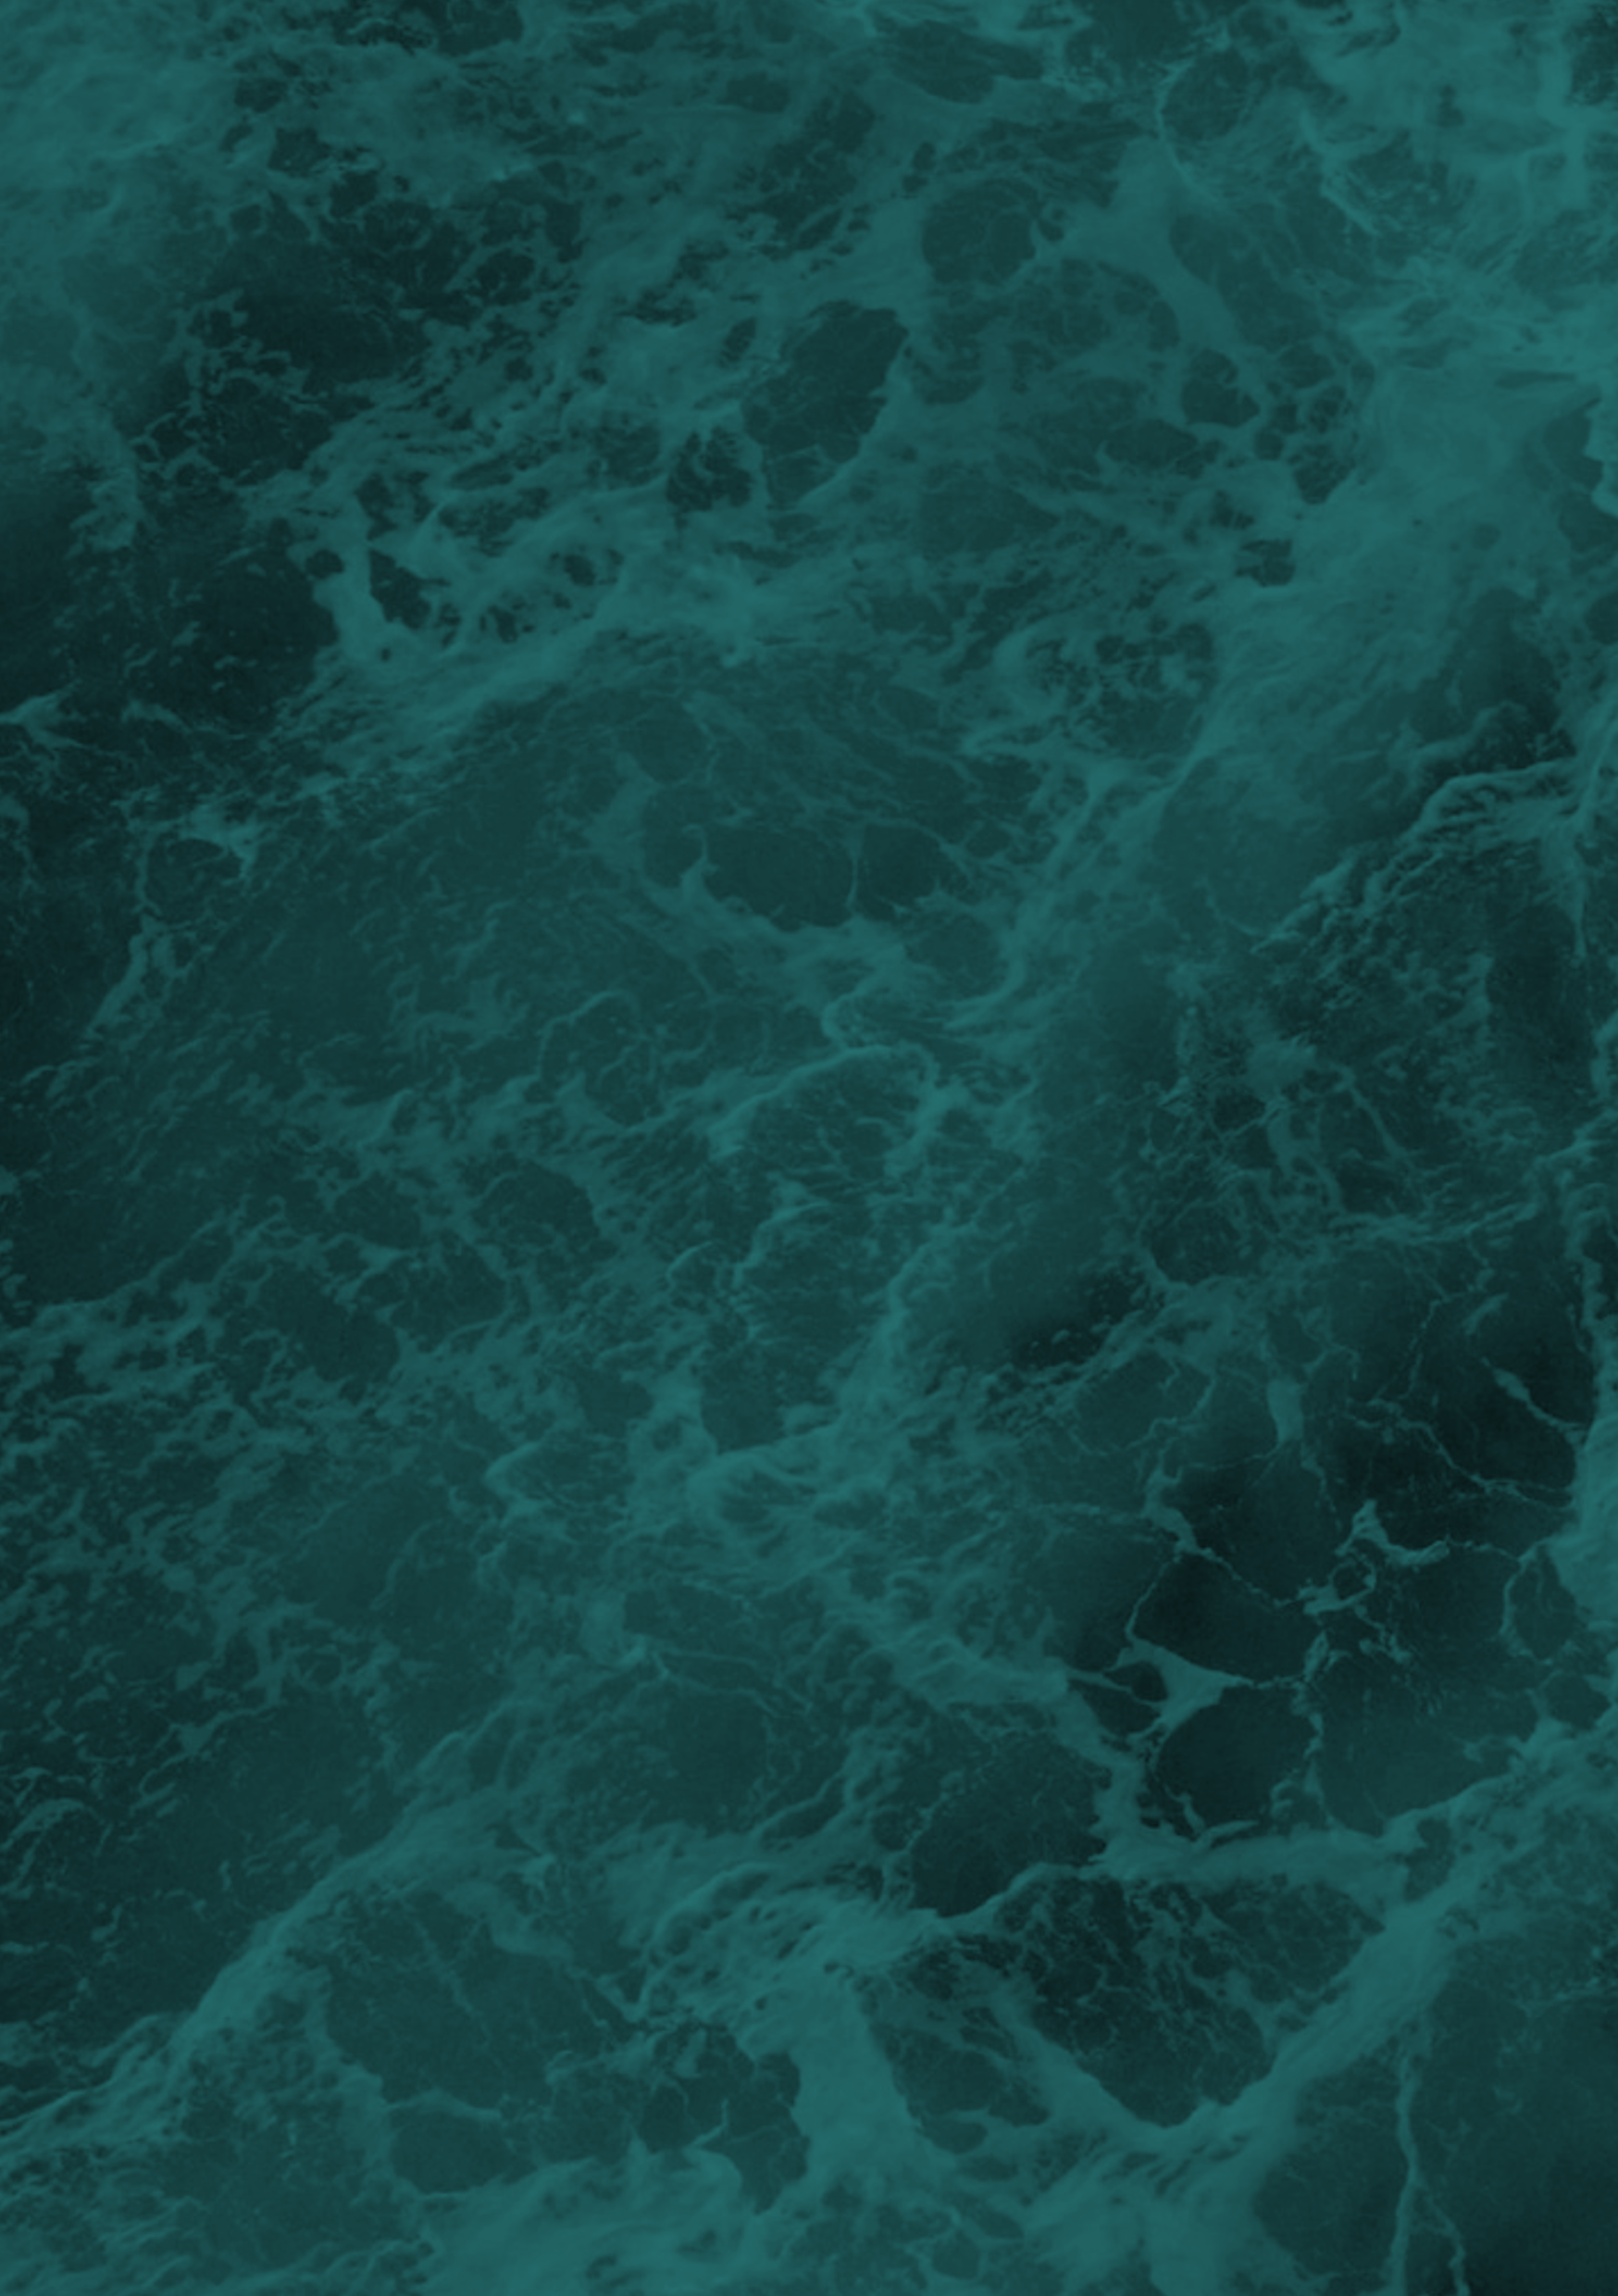
\includegraphics[width=\paperwidth,height=\paperheight]{img/fon.png}};
\noindent{\noindent
\fontsize{30}{30}\selectfont\bf
\color{white}
\noindentС.\,Н.\,ГУРБАТОВ\\[.2em]
\textcolor{white}{\rule{9cm}{3pt}}\\[.5em]
\fontsize{36}{36}\selectfont\bf
\noindentМЕХАНИКА\\[0.4em]
\noindentСПЛОШНЫХ\\[0.4em]
\noindentСРЕД}
\clearpage
\newpage
\end{titlepage}
% \end{document}

%!TEX root = lections.tex
% \newpage
\begin{titlepage}
\thispagestyle{empty}

\begin{flushleft}
УДК 532 \\
ББК 22.253.3\\

\end{flushleft}

\vskip 20pt

\hphantom{Г 95}{\bf Гурбатов С.Н.}\\
Г 95\hspace{1em} Лекции по механике сплошных сред --- \textcolor{red}{Изд. ННГУ}, \the\year. \\
\hphantom{Г 95\hspace{1em}} -- \pageref{LastPage} c., илл.\\[1.1em]
\hphantom{Г 95\hspace{1em}} ISBN \textcolor{red}{000-0-00000-000-0}
% 
% \begin{tabular}{ll}
%     & {\bf Гурбатов С.Н.} \\
% Г 95 & Лекции по механике сплошных сред \\
% 	&  --- \textcolor{red}{ИЗД-ВО}, 2020. - 110 c., илл. \\
% 	&  \\
% \end{tabular}

\vskip 30pt
\begin{center}
\it
Оформление и вёрстка: \\Сарафанов Ф.Г., Платонова М.В., Есюнин Д.В.
\end{center}
\vskip 30pt

{\small
Книга предназначена для студентов высших учебных заведений направления <<радиофизика>>. Она охватывает курс лекций, читаемый на 3 курсе профессором кафедры акустики радиофизического факультета ННГУ Сергеем Николаевичем Гурбатовым.
}
\vskip 100pt

\vfill
\begin{flushright}
УДК 532 \\
ББК 22.253.3
\end{flushright}

% \vskip 100pt

{\bf  ISBN \textcolor{red}{000-0-00000-000-0}} \hfill \copyright\,Гурбатов С.Н., \the\year
% \end{tabular}
\end{titlepage}

% \begin{titlepage}

\begin{center}

	\textsc{Нижегородский государственный университет имени Н.\,И. Лобачевского}
	\vskip 4pt \hrule \vskip 8pt
	\textsc{Радиофизический факультет}
	\vskip 60pt
	\Large{\textsc{Лекции по курсу механики сплошных сред}}
	\vfill


\end{center}

\vfill

\begin{flushright}
	{\sciadviser}
\end{flushright}

\vfill

\begin{center}
	Нижний Новгород, \the\year
\end{center}

\end{titlepage}
\renewcommand{\phi}{\varphi}
\renewcommand{\hat}{\widehat}
\newcommand{\const}{\mathrm{const}\,}
\newcommand{\frc}[2]{\raisebox{2pt}{$#1$}\big/\raisebox{-3pt}{$#2$}}
\tableofcontents

\newpage
\sloppy

% %!TEX root = ../main.tex
\section{Введение}

Курс \textbf{Механика сплошных сред}(далее \textbf{\textbf{МСС}}) является одним из разделов цикла теоретической физики.  Так в знаменитом курсе теоретической физики Л.Д.Ландау и Е.М.Лифшица  ему посвящено два достаточно объемных тома ( объем свыше 1000 страниц).

Наш курс для радиофизиков – он существенно меньше чем курсы на мехматах МГУБ НГУБ ННГУ.  Наш  курс рассчитан на радиофизиков, несколько больший объем в нем занимают волновые процессы. Похожие курсы читаются на физфаке МГУ (отделение радиофизики), Физтехе - МФТИ.

Следует отметить, что исходные уравнения механики сплошных сред существенно сложнее чем уравнения электродинамики, где базовыми являются линейные уравнения Максвелла. В тоже время, в этих курсах возникают одинаковые уравнения, это одна из причин почему курсу читаются параллельно. В этих курсах большую роль играют формулы векторного анализа.

История развития \textbf{\textbf{МСС}} полностью подтверждает наличие тесной связи между становлением науки и запросами практики.  \textbf{\textbf{МСС}} – одна из древнейших наук. Ее зарождение идет еще в античной древности.

Фамилии (но не годы жизни) знают все. Это:
\begin{itemize}
	\item Аристотель (384-322 г.г. до н.э)
	\item Архимед ((287-212 г.г. до н.э) – закон Архимеда
\end{itemize}
	Средние века:
\begin{itemize}
	\item Галилей (1564-1642)
	\item Паскаль (1623-1662) 
	\item Леонардо де Винчи (1452-1519)
	Это и летательные аппараты, закон Паскаля для давления, наблюдение гидродинамической турбулентности.
	\item Гюйгенс (1629-1695)
	\item Ньютон (1642-1727). В своих знаменитых \emph{«Началах»} он приводит теоретический вывод квадратичного закона сопротивления. Именно из законов Ньютона было проведено обобщение на сплошные среды и родилась новая наука «гидромеханика».
\end{itemize}
Это два академика Российской академии наук
\begin{itemize}
	\item Леонард Эйлер (1707-1789) – уравнение Эйлера
	\item Даниил Бернулли (1700-1782) -  уравнение Бернули
	\item Даламбер (1717-1783) – парадокс
\end{itemize}
Начало 19 века:
\begin{itemize}
	\item Лагранж (1736-1813)
	\item Коши (1789-1857)
\end{itemize}
Вязкая жидкость:
\begin{itemize}
	\item Анри Навье  (1785-1863)
	\item Стокс (1819-1903) – уравнение Навье-Стокса
\end{itemize}
Эксперименты с жидкостью:
\begin{itemize}
	\item Ж. Пуазейль (1799-1869)
\end{itemize}
Основы теории турбулентности:
\begin{itemize}
	\item Осборн Рейнольдс (1842-1912)
	\item Н.Е.Жуковский (1847-1921) Обтекание крыла, присоединённый вихрь, подъемная сила
	\item С.А.Чаплыгин (1869-1942)
	\item Морис Мари Альфред Куэтт  (1858-1943) – течение Куэтта
\end{itemize}
Теории турбулентности и теория устойчивости:
\begin{itemize}
	\item Людвиг Прандтль  (1875-1953)
	\item Теодор Карман (1881-1963)
\end{itemize}

Практически все эти фамилии будут встречаться в нашем курсе – их именами названы законы \textbf{МСС}.
В наше время бурное развитие получила вычислительная \textbf{МСС}. Так не один новый самолет не получит разрешение на эксплуатацию, если на будет построена его математическая модель, включающая процессы самолета  обтекания потоком.
Что включает современная \textbf{МСС}. В книге академика Л.Седова краткое перечисление современных проблем включает 21 пункт и занимает 4 страницы. Здесь мы приведем лишь те, которые тесно связаны с предприятиями и НИИ Нижнего Новгорода, и где работают выпускники радиофака

\begin{enumerate}
	\item Изучение движения жидкости и газа – движение самолетов, вертолетов, подводных лодок.  Возникновение турбулентных следов за объектами. Излучение звука винтами и турбулентными струями. ИПФ РАН, ОКБМ.
	\item Движение жидкости и газа в трубах. Взаимодействие волн в оболочках. ИПФ РАН, ОКБМ.
	\item Волновые движения в жидкостях и газах
	\begin{itemize}
		\item Волны в твердых телах.  Акустическая диагностика, взаимодействие с электромагнитными волнами – линии задержки на ПАВ (радиоэлектронной комплекс НО)
		\item Волны на поверхности моря и внутренние волны, их нелинейное взаимодействие. Обнаружение ПЛ по изменению характеристик поверхностного волнения.
		\item Волны в каналах, реках. Генерация цунами и  набег волн цунами на берег.
		\item Сейсмические процессы, нелинейная сейсмодиагностика.
		\item Звуковые волны,  гидроакустика, акустика океана
	\end{itemize}
	\item Теория турбулентности – гравитационная неустойчивость
	\item Биологическая механика, движение крови в сосудах, диагностика на различных типах волн – сдвиговые волны
\end{enumerate}
Пример – \textbf{Институт прикладной физики РАН}, один из крупнейших институтов Российской академии наук.
Филиалы:
\begin{itemize}
	\item \textbf{Институт физики микроструктур} РАН
	\item \textbf{Институт проблем машиностроения} РАН
\end{itemize}

\textbf{Федеральное государственное бюджетное научное учреждение «Федеральный исследовательский центр Институт прикладной физики Российской академии наук» (ИПФ РАН)} был создан на базе нескольких отделов Научно-исследовательского радиофизического института (НИРФИ) Минвуза РСФСР в апреле 1977 года. Основатель и директор института на протяжении первых 25 лет его работы — академик А. В. Гапонов-Грехов, с 2003 по 2015 год институт возглавлял академик А. Г. Литвак, с 2015 года до своего избрания президентом РАН в 2017 году директором института был академик А. М. Сергеев. С октября 2017 г. временно исполняющим обязанности директора ИПФ РАН назначен член-корреспондент РАН Г.Г. Денисов.
\section{Структура курса МСС}
\begin{enumerate}
	\item Введение
	\item Основные законы гидродинамики идеальной жидкости («сухая» вода по Ричарду Фейману)
	\item Движение вязкой несжимаемой жидкости («мокрая» вода)
	\item Элементы теории турбулентности
	\item Движение сжимаемой жидкости («звук»)
\end{enumerate}
\subsection{Литература к курсу}
\begin{enumerate}
\item Основная литература:
	\begin{enumerate}
		\item Ландау Л.Д., Лифшиц Е.М. Теоретическая физика, т. 6. Гидродинамика. М:  Физматлит, 2015 – 733 с
		\item Бреховских Л.М., Гончаров В.В. Введение в механику сплошных сред (в приложении к теории волн). М.: Наука, 1982. - 335 с
		\item Гурбатов С.Н., Грязнова И.Ю., Демин И.Ю., Курин В.В., Прончатов-Рубцов Н.В. Сборник задач по механике сплошных сред: гидромеханика и акустика (учебное пособие) Изд-во ННГУ, Н.Новгород, 2006. - 92 с.
		\item Акустика в задачах. Учеб. рук-во. / Под ред. С.Н.Гурбатова и О.В.Руденко. М.: Наука, 2009. - 336 с.
	\end{enumerate}
\item Дополнительная литература:
	\begin{enumerate}
		\item Кочин Н.Е., Кибель И.А., Розе Н.В. Теоретическая гидродинамика. Т.1, 2. М: Физматлит, 1963.
		\item Бетчеллор Дж. Введение в механику жидкости. М: Наука, 1970. 
		\item Фейман Р., Лейтон Р., Сэндс М. Феймановские лекции по физике, т. 7. Физика сплошных сред. М: Мир, 1977.
		\item Лойцянский Л.Г. Механика жидкости и газа. М: Дрофа, 2003. 840 с.
		\item Лайтхилл Д. Волны в жидкостях. М: Мир, 1981. 589 с.
		\item Седов Л.И. Механика сплошных сред. В 2-х т. СПб: Лань, 2004. 528 с. и 560 с.
		\item Островский Л.А. Вопросы динамики жидкости. Учебное пособие. Горький, ГГУ, 1982. – 145 с.
	\end{enumerate}
\item Программное обеспечение и Интернет-ресурсы:
	\begin{enumerate}
		\item Гурбатов С.Н., Грязнова И.Ю., Демин И.Ю., Курин В.В., Прончатов-Рубцов Н.В.  Электронный задачник «Основы механики сплошных сред: гидромеханика и акустика»  Фонд образовательных электронных ресурсов ННГУ, 2012. – 95 с. \url{http://www.unn.ru/books/met_files/Zadachnic_MSS.doc}
		\item Грязнова И.Ю., Мартьянов А.И. "Экспериментальные исследования закономерностей обтекания цилиндра и крыла воздушным потоком на аэростенде ТМЖ-1М". Электронное учебно-методическое пособие.  Фонд образовательных электронных ресурсов ННГУ, 2012. – 60 с. \url{http://www.unn.ru/books/resources.html}
		\item Курин В.В., Грязнова И.Ю., Клемина А.В., Мартьянов А.И. УМК "Основы механики сплошных сред" Фонд образовательных электронных ресурсов ННГУ, 2011. – 88 с. \url{http://www.unn.ru/books/resources.html}
	\end{enumerate}
\end{enumerate}
\subsection{Основные допущения \textbf{МСС}}
Вещество можно рассматривать как непрерывную сплошную среду, пренебрегая его молекулярным строением. И однвременно считаем непрерывным распределение всех характеристик жидкости (плотность, скорость, температура, $\ldots$).

Это означает, что всякий малый элемент жидкости или газа содержит большое число молекул(или других частиц ). То есть когда мы говорим о бесконечно малом элементе жидкости, то везде мы подразумеваем,  что \emph{«физически»} бесконечно малый объем мал по сравнению с размерами тел, но велик по сравнению с межмолекулярными расстояниями.

Это позволяет применить в \textbf{МСС} хорошо разработанный для непрерывных функций аппарат высшей математики.

Нетривиальный пример – \textbf{крупномасштабная структура Вселенной.}

Описание развития крупномасштабной структуры  уравнениями гидродинамики газа гравитационно взаимодействующих частиц. \emph{«Физически»} бесконечно малый объем – объем в котором содержится много галактик.

Существующие на данный момент крупномасштабные образования возникли из-за малых начальных возмущений плотности за счет гравитационной неустойчивости. Обычная материя (атомов различных веществ) (4\%), Темная материя неизвестной физической природы (cold dark matter) (23\%). Темная энергия (dark energy) (73\%), которая играет антигравитационную роль в процессе формирования Вселенной.

Плотность темного вещества в 6–7 раз превосходит плотность барионов, и поэтому рост неоднородностей определяется в основном темным веществом. Именно рост неоднородностей в темном веществе и ответственен за формирование крупномасштабных структур. Барионная компонента просто следовала за эволюцией темного вещества.

В космологии понятие крупномасштабной структуры относится к распределению галактик и массы темного вещества (на масштабах от одного до нескольких сотен мегапарсек). Современная теория объясняет формирование крупномасштабной структуры Вселенной как следствие роста исходных слабых флуктуаций плотности вещества за счет гравитационной неустойчивости. При этом формирование ярко выраженных элементов структуры происходит на нелинейной стадии. Именно поэтому процесс формирования крупномасштабной структуры принято иногда гравитационной турбулентностью.

Наиболее очевидный путь преодоления сложности учета законов нелинейной эволюции гравитационной неустойчивости на поведение поля плотности вещества состоит в численном моделировании трехмерного движения $N$ гравитационно взаимодействующих частиц. Альтернативой являются приближенные аналитические решения некоторых уравнений в частных производных, адекватно описывающих рост флуктуаций неоднородной плотности вещества в расширяющейся Вселенной. Первый из этих подходов был предложен Зельдовичем в 1970 году. (Зельдович Я Б Астрофизика 6 319 (1970); Zeldovich Ya B Astrophys. 6 164 (1970); Zeldovich Ya B Astron. Astrophys. 5 84 (1970)

Второй аналитический подход к проблеме описания формирования крупномасштабной структуры Вселенной (1) базируется на векторном уравнении Бюргерса. В данном подходе многопотоковое движение гравитационно взаимодействующих частиц в особенностях, приводящее к их локализации, моделируется вязким слагаемым в уравнении Бюргерса. В предельном случае исчезающе малой вязкости это эквавалентно слипанию частиц и поэтому данный подход часто называют приближением слипания - adhesion model (см., например, (2-5). 

Adhesion model Модель Зельдовича-Гурбатова-Саичева
Предельная версия модели слипания естественным образом описывает характерную мозаичную структуру распределения вещества во Вселенной. Основные элементы “мозаики” в трехмерном пространстве (вершины, ребра, грани и внутренности ячеек) могут быть ассоциированы с наблюдаемыми структурами трехмерного распределения галактик (компактные скопления галактик, филаменты – цепочки галактик, поверхности со сравнительно высокой плотностью галактик, и темные области между ними, бедные галактиками).

Сама эволюция крупномасштабной структуры Вселенной может трактоваться как непрерывый процесс транспортировки вещества преимущественно из объектов большой размерности к объектам мозаичной структуры, обладающим меньшей размерностью. К примеру, вещество из внутренних ячеек мозаичной структуры (трехмерных объектов) перетекает в ее грани (квазидвумерные объекты), а из них в ребра и вершины мозаичной структуры. В то же время, сами ячейки участвуют в непрерывном движении, деформации и поглощении одних ячеек другими.

(1) Gurbatov S.N., Saichev A.I., \& Shandarin S.F. 1989, Mon. Not. R. astr. Soc., 236, 385

(2) Гурбатов С.Н., Малахов А.Н., Саичев А.И. Нелинейные случайные волны в средах без дисперсии. М.: Наука, 1990. 215 с. Сер. Современные проблемы.

Gurbatov S.N., Malakhov A.N., Saichev A.I. Nonlinear random waves and turbulence in nondispersive media: waves, rays and particles. — Manchester University Press, 1991. — 308 p.

(3) Vergassola M., Dubrulle B., Frisch U., Noullez A. 1994, Astron. Astrophys. 289. 325.

(4) Гурбатов С. Н., Саичев А. И., \& Шандарин С. Ф.   «Крупномасштабная структура Вселенной. Приближение Зельдовича и модель слипания»,  УФН, 182,  233–261 (2012)

(5) Гурбатов С.Н., Руденко О.В., Саичев А.И. Волны и структуры в нелинейных средах без дисперсии. Приложения к нелинейной акустике. М.: Физматлит, 2008.

Gurbatov S.N.,Rudenko O.V., \& Saichev A.I. Waves and Structures in Nonlinear Nondispersive Media. General Theory and Applications to Nonlinear Acoustics. — Springer-Verlag, Berlin, Heidelberg, Germany, 2012. — 472 p . с
\begin{figure}[tb]
	\centering
	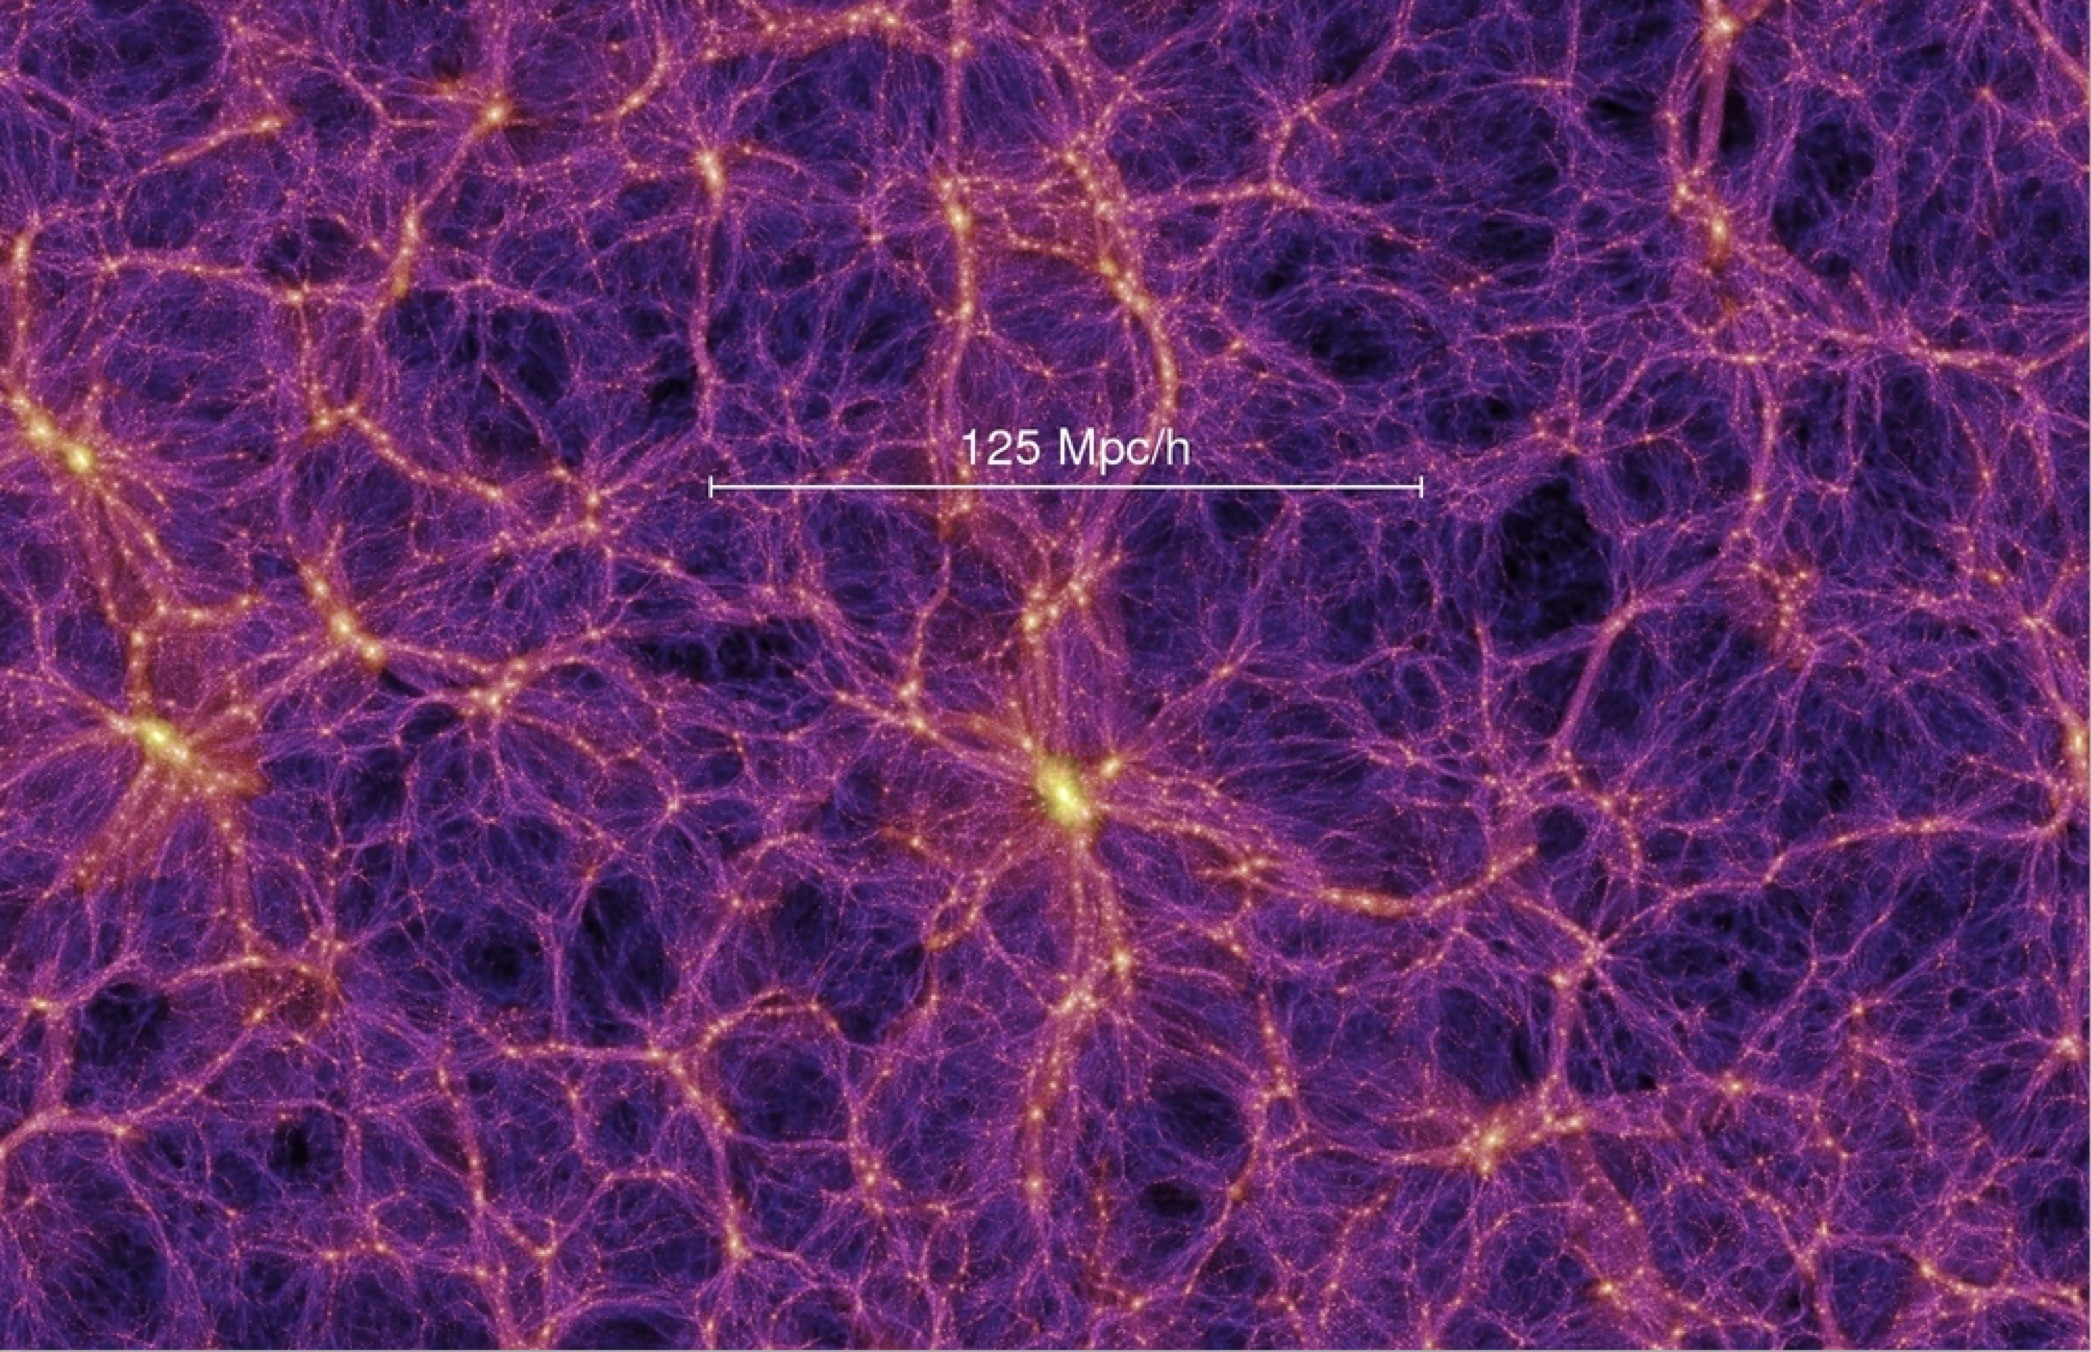
\includegraphics[width=.6\linewidth]{photo/1.jpg}
	\caption{Крупномасштабная структура Вселенной}
	\label{fig:figure1}
\end{figure}
\begin{figure}[tb]
	\centering
	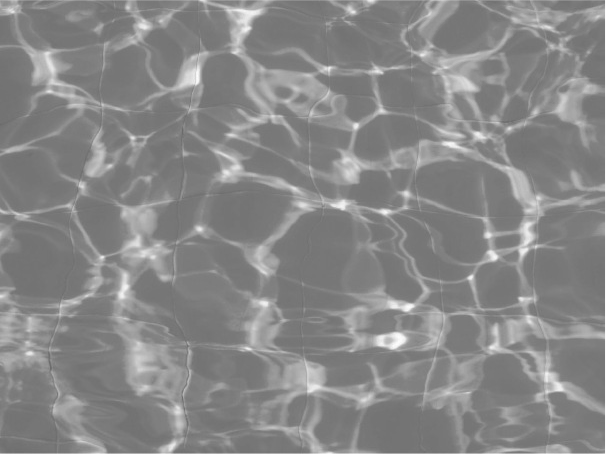
\includegraphics[width=.6\linewidth]{photo/2.png}
	\caption{Система каустик на дне бассейна}
	\label{fig:figure2}
\end{figure}
В заключение отметим, что результаты динамического моделирования в рамках приближения слипания можно посмотреть на Youtube (\textbf{The Sticky Geometry of the Cosmic Web, version 2.01})

\url{https://www.youtube.com/watch?v=wI12X2zczqI}

Результаты прямого численного моделирования (N-body simulation) можно также  посмотреть на Youtube

Двухмерный случай:

\url{https://www.youtube.com/watch?v=nHvcqV92oqY}

\url{https://www.youtube.com/watch?v=74IsySs3RGU}

Трехмерный случай

\url{https://www.youtube.com/watch?v=eDGtFRj4xXc}

\newpage
\section{Основные уравнения гидродинамики идеальной жидкости}

В  данном разделе мы рассмотрим законы движения и равновесия идеальной жидкости, то есть жидкости в которой не учитывается внутреннее трение, и следовательно, нет перехода механической энергии в тепловую. Будем также пренебрегать теплообменом между  различными объемами жидкости.

Это означает что все процессы протекают при постоянной энтропии. И напряженное состояние жидкости характеризуются одной скалярной величиной $P$ – давлением. Это конечно идеализация, которая приводит к ряду парадоксальных результатов (например, парадокс  Даламбера-Эйлера о том, что сила сопротивления при равномерном движении тела в жидкости равна нулю). Тем не менее, без этой идеализации невозможно дальнейшее изучение реальных ситуаций.
\subsection{Основные уравнения гидродинамики идеальной жидкости}
Прежде чем перейти к выводу уравнений рассмотри два альтернативных способа описания движения жидкости. Оба они были предложены Леонардом Эйлером, но одно из них носит имя Лагранжа.
\begin{center}
{\emph{Первый способ} – \textbf{Лагранжево описание}}
\end{center}
В основу этого способа положено описание движения отдельных «жидких частиц». При этом все величины, в том числе и  координаты частицы жидкости определятся как функции времени $t$  и некоторых переменных $\xi_i(i=1,2,3)$, идентифицирующих определенную частицу («метки» частиц)
\begin{align*}
	x_i &=x_i(\xi_k,t) \\
	P &=P(\xi_k,t) \\
	\rho &=\rho(\xi_k,t) \\
	\ldots 
\end{align*}
В качестве переменных $\xi_k$ обычно используют начальные координаты частиц жидкости
\begin{align*}
	t &=t_0 \\
	\xi_i &= x_i(\xi_k,t_0)
\end{align*}

Таким образом при лагранжевом описании мы следим за определленными частицами жидкости и смотрим как изменяются во времени их координаты,  скорости, ускорения, а также давление, температура, плотность в их окрестности.

При этом скорость и ускорение частицы вычисляются как
\begin{align*}
v_{i} &=\frac{\partial x_{i}}{\partial t} \\
a_{i} &=\frac{\partial^{2} x_{i}}{\partial t^{2}} 
\end{align*}
Здесь $ \vec{v}\left(\xi_{k}, t\right) $ - скорость частицы в момент времени $t$ имела координаты $\xi_1,\xi_2,\xi_3$.

Отметим, что такому описанию соответствует способ исследования океана (реки Волги) с помощью геофизических буев с нулевой плавучестью.
\begin{figure}[H]
	\centering
	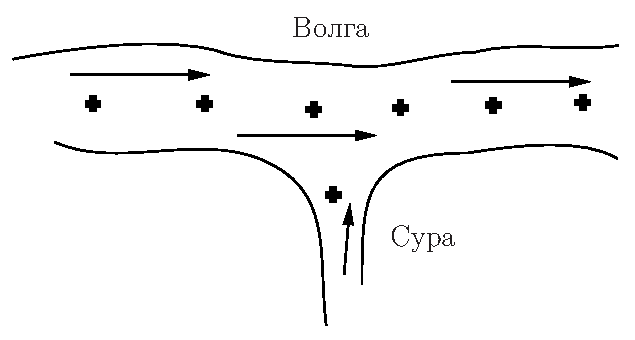
\includegraphics[scale=1]{photo/3.pdf}
	\caption{Схематичная картина Лагранжева и Эйлерова описания. \ding{58} - якорь.}
	\label{fig:figure3}
\end{figure}
\begin{center}
	{\emph{Второй способ} – \textbf{Эйлерово описание}}
\end{center}

Неподвижное пространство заполнено движущейся жидкостью. Движение жидкости будет определено если все величины характеризующую жидкость (скорость движения, давление, плотность, температура и т.д.) \textcolor{red}{будут определены}.
То есть мы следим, как меняются эти величины от точки к точке
\begin{align*} 
\vec{v} &=\vec{v}(\vec{x}, t) \\
T &=T(\vec{x}, t)
\end{align*}
Система заякоренных буев. 
В Эйлеровом описании мы не знаем что делается с отдельной частицей. При этом частные производные от скорости не являются ускорением. Так если течение стационарно и частная производная по времени  равна нулю, частицы в данной точке могут иметь ускорение. Пример – водопад.

Найдем ускорение частицы. За время $ \Delta t $ частица находящаяся в момент времени $t$ в точке с координатами $ x_{k} $ переместится в точку $ x_{k}=x_{k}+\Delta x_{k} $. Тогда для $i$-ой компоненты ускорения имеем
\begin{align*} 
\lim _{\Delta t \rightarrow 0} \frac{\Delta x_{k}}{\Delta t} &=\frac{\partial x_{k}}{\partial t}=v_{k} 
\end{align*}
\begin{align*}
a_{i} &=\lim _{\Delta t \rightarrow 0} \frac{v_{i}\left(x_{k}+\Delta x_{k}, t+\Delta t\right)-v_{i}\left(x_{k}, t\right)}{\Delta t} \\
&=\lim _{\Delta t \rightarrow 0}\frac{\left[v_{i}\left(x_{k}, t\right)+\frac{\partial v_{i}}{\partial x_{k}} \Delta x_{k}+\frac{\partial v_{i}}{\partial t}-v_{i}\left(x_{k}, t\right)\right]}{\Delta t} \\
&=\frac{\partial v_{i}}{\partial x_{k}} v_{k}+\frac{\partial v_{i}}{\partial t} \\
\end{align*}
Таким образом 
\begin{align*} 
a_{i} &=\frac{\partial v_{i}}{\partial t}+v_{k} \frac{\partial v_{i}}{\partial t}=\left(\frac{\partial}{\partial t}+v_{k} \frac{\partial}{\partial t}\right) v_{i} \\
\vec{a} &=\frac{\partial \vec{v}}{\partial t}+(\vec{v} \nabla) \vec{v}=\left(\frac{\partial}{\partial t}+(\vec{v} \nabla)\right) \vec{v}
\end{align*}

Аналогично находятся и производные от любой другой величины. Эта производная носит название субстанциональной производной.
\begin{align*} 
\frac{d}{d t}=\frac{\partial}{\partial t}+(\vec{v} \nabla)
\end{align*}
\subsection{Переход от Эйлерова описания к Лагранжеву и обратно}
Пусть известно Эйлерово поле скорости $ \vec{v}=\vec{v}(\vec{x}, t) $. Чтобы найти как двигаются Лагранжевы частицы $ \vec{x}(t, \vec{\xi}) $ нужно решить уравнение
\begin{align*} 
\frac{d \vec{x}}{d t}=\vec{v}(\vec{x}, t) \\
\vec{x}(t=0, \vec{\xi})=\vec{\xi}
\end{align*}
Как найти эйлерово поле скорости? Если нам известно поведение лагранжевых частиц $ \vec{x}(t, \vec{\xi}) $, то вначале нам нужно решить уравнение 
\begin{align*} 
\vec{x}=\vec{x}(t, \vec{\xi})
\end{align*}

Решение этого уравнения 
\begin{align*} 
\vec{\xi}=\vec{\xi}(\vec{x}, t)
\end{align*}
позволяет найти Лагранжеву частицу, которая в момент времени $t$ попала в точку $x$. Тогда эйлерово поле скорости будет равно
\begin{align*} 
\vec{v}(\vec{x}, t)=\vec{v}(t, \vec{\xi}(\vec{x}, t)
\end{align*}
\subsection{Уравнение непрерывности и закон сохранения массы}
Пусть имеется некоторый объем пространства $V$ заполненный движущейся  жидкостью. Количество жидкости (масса) в этом объеме равно:
\begin{align*} 
m=\int\limits_{V} \rho d V
\end{align*}
где $\rho$ - плотность жидкости. Жидкость может притекать и вытекать из объема. Введем элемент поверхности $ d \sigma $ и вектор $ d \vec{\sigma}=d \sigma \vec{n} $, направленный по внешней нормали к поверхности. 
\begin{figure}[H]
	\vspace{-10pt}
	\centering
	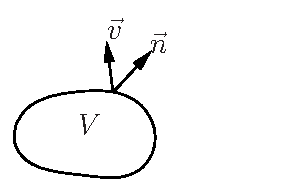
\includegraphics[scale=1]{photo/4.pdf}
	\caption{Объем, скорость и нормаль к поверхности}
	\label{fig:figure4}
\end{figure}
Поток через элемент поверхности определяется скалярным произведением:
\begin{align*}
\oint\limits_{S} \rho \vec{v} d \vec{\sigma}=\int\limits_{V} \Div(\rho \vec{v}) d V
\end{align*}


Уравнение баланса имеет вид:
\begin{align*} 
\frac{\partial}{\partial t} \int\limits_{V} \rho d V=-\oint\limits_{S} \rho \vec{v} d \vec{\sigma}
\end{align*}
Это интегральный закон сохранения массы. Если на поверхности скорость равна нулю, то масса сохраняется.

Используя формулу Остроградского-Гаусса
\begin{align*} 
\oint\limits_{S} \rho \vec{v} d \vec{\sigma}=\int\limits_{V} \operatorname{div}(\rho \vec{v}) d V
\end{align*}
получим 
\begin{align*} 
\int\limits_{V}\left[\frac{\partial \rho}{\partial t}+\Div(\rho \vec{v})\right] d V=0
\end{align*}

Так как объем произвольный, то мы получаем дифференциальный закон сохранения
\begin{align*} 
\frac{\partial \rho}{\partial t}+\Div(\rho \vec{v})=0
\end{align*}

Вектор $ \vec{j}=\rho \vec{v} $ - плотность потока массы. Используя формулу $ \nabla(a \vec{b})=\nabla a \vec{b}+a \nabla \vec{b} $, перепишем закон сохранения массы в виде:
\begin{align*} 
\frac{\partial \rho}{\partial t}+(\vec{v} \nabla) \rho+\rho \Div(\vec{v})=0 \\
\frac{d \rho}{d t}=-\rho \Div(\vec{v})=0
\end{align*}

\textbf{Несжимаемая жидкость - плотность вдоль траектории частицы не меняется.}
\begin{align*} 
\frac{d \rho}{d t}=0
\end{align*}
То есть поле скорости соленоидально $\Div\vec{v}=0$.
% %!TEX root = ../lections.tex
\subsection{Уравнение Эйлера}
Уравнение движение идеальной жидкости ( аналог \textbf{2 закона Ньютона})
Второй закон Ньютона для жидкого элемента
\begin{align*}
\rho d V \frac{d \vec{v}}{d t} &=\vec{F_{S}}+\vec{F} \\
\vec { F } &= \rho \vec { f }
\end{align*}
Здесь $F$ объемная сила действующая на элемент $dV$ ( $f$ – сила отнесенная к единице массы, для силы тяжести $f=g$, где g ускорение свободного падения).

$F_s$ - сила действующая на элемент объема со стороны окружающей среды.  В идеальной среде силы трения нет и единственная сила определяется только силами давления. На элемент поверхности $d\sigma$ действует сила $ P d \vec { \sigma } $ и результирующая сила равна:
\begin{align*}
\vec { F } _ { S } = - \oint \limits_ { S } p d \vec { \sigma } = - \int \limits_ { V } \nabla p d V \approx - \nabla p d V
\end{align*}

В результате получаем \textbf{уравнение Эйлера}
\begin{align*}
\frac { d \vec { v } } { d t } = - \frac { \nabla p } { \rho } + \vec { f }
\frac { \partial \vec { v } } { \partial t } + ( \vec { \vec{v} } \nabla ) \vec { v } = - \frac { \nabla p } { \rho } + \vec { f }
\end{align*}
Здесь мы учли что в уравнение Ньютона входит полная производная. У нас  5 неизвестных – 3 компоненты скорости, давление и плотность. И только 4 уравнения: 3 уравнения Эйлера для трех компонент и уравнение непрерывности.
Нужно еще одно уравнение – уравнение состояния, связывающее давление, плотность и энтропию $S$: $ P = P ( \rho , S ) $ и уравнение для энтропии. Для изоэнтропический жидкости $ \frac { d S } { d t } = \frac { \partial S } { \partial t } + \vec { v } \nabla S = 0 $

Если в начальный момент времени энтропия была одинакова во всем пространстве, то она не будет меняться с течением времени и уравнение состояние принимает вид: $ P = P ( \rho ) $.
В идеальном газе уравнение адиабаты имеет вид(\textbf{уравнение Пуассона}):
\begin{align*}
P &= P _ { 0 } \left( \rho / \rho _ { 0 } \right) ^ { \gamma } \\
\gamma &= c _ { p } / c _ { v }
\end{align*}
где для идеального газа $\gamma = \frac{i+2}{i}$, ($i$ - количество степеней свободы).
Для жидкостей дело хуже. В разных диапазонах давления имеют разные уравнения состояния. Эмпирическая формула для давления $P$, измеряемого в атмосферах: 
\begin{align*}
\frac { P + B } { 1 + B } = \left( \frac { \rho } { \rho _ { 0 } } \right) ^ { \gamma }
\end{align*}
где $B=3000\text{ атм}$, $\gamma = 7$, давление до $10^5$ атмосфер.

Итак, \textbf{система уравнений для идеальной жидкости} принимает вид:
\begin{align*}
& \frac { \partial \vec { v } } { \partial t } + ( \vec { v } \nabla ) \vec { v } = - \frac { \nabla p } { \rho } + \vec { g } \\
& \frac { \partial \rho } { \partial t } + d i v ( \rho \vec { v } ) = 0 \\
& P = P ( \rho )
\end{align*}
\subsection{Законы сохранения энергии и импульса для идеальной жидкости}

Энергия единицы объема – кинетическая $+$ внутренняя
\begin{align*}
E = \frac { 1 } { 2 } \rho v ^ { 2 } + \rho \varepsilon
\end{align*}

Закон сохранения энергии в интегральной форме:
\begin{align*}
\frac { \partial } { \partial t } \int\limits_{ V } \rho \left( \frac { 1 } { 2 } v ^ { 2 } + \varepsilon \right) d V = - \oint\limits_{ S } \rho \left( \frac { 1 } { 2 } v ^ { 2 } + \varepsilon \right) \vec { v } d \vec { \sigma } - \oint _ { S } p \vec { v } d \vec { \sigma }
\end{align*}

Изменение энергии в объеме равно притоку (выносу) энергии в объем через границы $+$ работа внешних сил давления. Энтальпия равна $ W = \rho \varepsilon + P $ из курса термодинамики и общей физики. Получаем закон сохранения в интегральной форме:
\begin{align*}
\frac { \partial } { \partial t } \int \limits_{ V } \rho \left( \frac { 1 } { 2 } v ^ { 2 } + \varepsilon \right) d V = - \oint \limits_{ S } \rho \left( \frac { 1 } { 2 } v ^ { 2 } + W \right) \vec { v } d \vec { \sigma }
\end{align*}
По формуле Стокса переходим в правой части от интегрирования по поверхности к интегрированию по объему:
\begin{align*}
\int \limits_ { V } \left[ \frac { \partial } { \partial t } \rho \left( \frac { 1 } { 2 } v ^ { 2 } + \varepsilon \right) + \Div \left( \rho \left( \frac { 1 } { 2 } v ^ { 2 } + W \right) \vec { v } \right] d V = 0\right.
\end{align*}

Поскольку объем произвольный можно перейти к дифференциальной  форме закона сохранения энергии:
\begin{align*}
& \frac { \partial E } { \partial t } + \Div \vec { N } = 0 \\
& E = \frac { \rho v ^ { 2 } } { 2 } + \rho \varepsilon \\
& \vec { N } = \left[ \frac { \rho v ^ { 2 } } { 2 } + \rho \varepsilon + P \right] \vec { v }
\end{align*}
Здесь $E$ – плотность энергии, $N$ – вектор плотности потока энергии – аналог вектора Пойнтинга в электродинамике. Введён в 1874 году Умовым.

\subsection{Закон сохранения импульса}
Для единицы объема жидкости импульс равен $ \vec { p } = \rho \vec { v } $. Если закон сохранения энергии мы выводили в интегральной форме, то здесь мы будем стартовать с дифференциальных уравнений. Запишем изменения для i-ой компоненты:
\begin{align*}
\frac { \partial } { \partial t } \left( \rho v _ { i } \right) = \rho \frac { \partial v _ { i } } { \partial t } + v _ { i } \frac { \partial \rho } { \partial t }
\end{align*}

Запишем уравнение Эйлера и уравнение непрерывности по компонентам:
\begin{align*}
\frac { \partial v _ { i } } { \partial t } + \sum _ { k = 1 } ^ { 3 } v _ { k } \frac { \partial v _ { i } } { \partial t } &= - \frac { 1 } { \rho } \frac { \partial P } { \partial x _ { i } } + f _ { i } \\
\frac { \partial \rho } { \partial t } + \sum _ { k = 1 } ^ { 3 } \frac { \partial \left( \rho v _ { k } \right) } { \partial x _ { k } } &= 0
\end{align*}
В результате для изменения компоненты импульса имеем:
\begin{align*}
\frac { \partial } { \partial t } \left( \rho v _ { i } \right) = - \frac { \partial } { \partial x _ { k } } \left( P \delta _ { i k } + \rho v _ { i } v _ { k } \right) + \rho f _ { i }
\end{align*}
Здесь по индексу $k$ идет суммирование. Хочетсяя привести это уравнение к дивергентной форме, чтобы получить закон сохранения. Учтем:
\begin{align*}
\rho v _ { k } \frac { \partial v _ { i } } { \partial x _ { k } } + v _ { i } \frac { \partial \left( \rho v _ { k } \right) } { \partial x _ { k } } = \frac { \partial \left( \rho v _ { i } v _ { k } \right) } { \partial x _ { k } }
\end{align*}
Внешние силы приводят к иземенеию импульса. Нужно что-то придумать с давлением:
\begin{align*}
\frac { \partial P } { \partial x _ { i } } = \frac { \partial \left( \delta _ { i k } p \right) } { \partial x _ { k } }
\end{align*}
Здесь $ \delta _ { i k } = 1 , i = k ; \delta _ { i k } = 0 , i \neq k $ - символ Кронекера.

В результате получим:
\begin{align*}
\frac { \partial } { \partial t } \left( \rho v _ { i } \right) = - \frac { \partial } { \partial x _ { k } } \left( P \delta _ { i k } + \rho v _ { i } v _ { k } \right) + \rho f _ { i }
\end{align*}

Введем тензор плотности потока импульса: $ \Pi _ { i k } = P \delta _ { i k } + \rho v _ { i } v _ { k } $. Тогда закон сохранения импульса запишется как:
\begin{align*}
\frac { \partial } { \partial t } \left( \rho v _ { i } \right) = - \frac { \partial \Pi _ { i k } } { \partial x _ { k } } + \rho f _ { i }
\end{align*}

Проинтегрируем последнее равенство по объему:
\begin{align*}
\frac { \partial } { \partial t } \int \limits_{ V } \rho v _ { i } d V = - \int \limits_{ V } \frac { \partial \Pi _ { i k } } { \partial x _ { k } } d V + \int \limits_{ V } \rho f _ { i } d V
\end{align*}
Используя теорему Остроградского-Гаусса для тензора получаем:
\begin{align*}
\frac { \partial } { \partial t } \int \limits_ { V } \rho v _ { i } d V = - \oint \limits_ { S } \Pi _ { i k } n _ { k } d \sigma + \int \limits_ { V } \rho f _ { i } d V
\end{align*}
Таким образом, изменение импульса в объеме $V$ связано с потоком импульса через поверхность $S$. Векторная же форма закона сохранения импульса имеем вид:
\begin{align*}
\frac { \partial } { \partial t } \int \limits_ { V } \rho  \vec{v} d V  = - \oint \limits_ { S } [ P \vec { n } + \rho \vec { v } ( \vec { v } \vec{n} ) ]d \sigma
\end{align*}
Здесь $\vec{n}$ - внешняя нормаль.

Следствие: Как использовать закон сохранения импульса для нахождения силы действия потока на тело? Если движение стационарно:
\begin{align*}
\oint _ { S } \left[ p n _ { i } + \rho v _ { i } v _ { k } n _ { k } \right] d \sigma = 0
\end{align*}
Отсюда для силы действия потока на тело имеем:
\begin{align*}
F _ { i } = - \oint \limits_ { S } p n _ { i } d \sigma = \oint \limits_ { S } \rho v _ { i } v _ { k } n _ { k } d \sigma
\end{align*}

Пример - изогнутая трубка(душ).
\begin{align*}
\frac { \partial } { \partial t } \int \limits_ { V } \rho  \vec{v} d V  = - \oint \limits_ { S } [ P \vec { n } + \rho \vec { v } ( \vec { v } \vec{n} ) ]d \sigma
\end{align*}
\begin{figure}[H]
	\centering
	\includegraphics[]{example-image-a}
	\caption{картинка изогнутой трубки}
	\label{fig:figure5}
\end{figure}
В одно сечение жидкость втекает, а из другого вытекает.
\subsection{Гидростатика}
Рассмотрим простейший случай когда скорость жидкости равна нулю. Из исходной системы уравнений 
\begin{align*}
& \frac { \partial \vec { v } } { \partial t } + ( \vec { v } \nabla ) \vec { v } = - \frac { \nabla p } { \rho } + \vec { f } \\
& \frac { \partial \rho } { \partial t } + d i v ( \rho \vec { v } ) = 0 \\
& P = P ( \rho )
\end{align*}
следует
\begin{align*}
& \nabla P = \rho \vec { f } \\
& P = P ( \rho )
\end{align*}

Пусть внешняя сила потенциальна
\begin{align*}
& \vec { f } = - \nabla u \\
& \nabla P = - \rho \nabla u
\end{align*}
то есть градиенты давления и сила параллельны.

При какой зависимости плотности от координаты последнее уравнение имеет решение? Применим к последнему уравнению операцию ротора
\begin{align*}
& \operatorname { rot } ( \nabla P ) = 0 \\
& \operatorname { rot } ( - \rho \nabla u ) = - \rho \operatorname { rot } ( \nabla P ) - [ \nabla P \nabla \rho ] \\ 
& [ \nabla P \nabla \rho ] = 0
\end{align*}
Таким образом вектора градиентов плотности и потенциала должны быть параллельны.

\emph{Распределение давления в поле тяжести.}
\begin{align*}
& \nabla P = \rho \vec { g } \\
& P = P ( \rho )
\end{align*}
то есть в поле тяжести стационарное решение существует, если плотность зависит от высоты.

\textbf{Примеры:}
\begin{enumerate}
	\item {\textbf{Жидкость в поле тяжести}(вода). Плотность постоянна. Ось $z$ направлена вниз.
	\begin{align*}
	& \frac { d P } { d z } = \rho _ { 0 } g \\
	& P = P _ { A } + \rho _ { 0 } g z
	\end{align*}
	Давление увеличивается на 1 атмосферу на 10 метрах.}
	\item {\textbf{Изотермическая атмосфера}(идеальный газ с постоянной температурой $T$). Ускорение можно считать постоянным. Ось $z$ направлена вверх.
	\begin{align*}
	& \frac { d P } { d z } = - \rho ( z ) g \\
	& P = \frac { R } { \mu } \frac { m } { V } T \\
	& P = \frac { R } { \mu } \rho T
	\end{align*}
	Здесь $R$ - универсальная газовая постоянная. $\mu$ - молярная масса газа.
	\begin{align*}
	& \frac { R T } { \mu } \frac { d P } { d z } = - \rho ( z ) g \\
	& \rho = \rho _ { 0 } \exp ( - z / h ) , P = P _ { 0 } \exp ( - z / h ) \\
	& h = \frac { R T } { \mu g }
	\end{align*}
	Здесь $h$ - высота атмосферы, величина порядка 8 км, поэтому изменением силы тяжести можно пренебречь.}
	\item {\textbf{Закон Архимеда}. На тело, погруженное в жидкость,  со стороны жидкости действует выталкивающая сила, равная весу жидкости, вытесненную этим телом.
	\begin{align*}
	\nabla P = \rho \vec { g }
	\end{align*}
	Сила со стороны жидкости на элемент поверхности $ d \vec { F } = - p \vec { n } d S $. Здесь $\vec{n}$ - внешняя нормаль. Тогда сила Архимеда равна:
	\begin{align*}
	& \vec { F }_ { A }  = - \oint \limits_ { S } P \vec{n} d S = - \int \limits_ { V } \nabla P d V = - \int \limits_ { V } \rho \vec { g } d V \\
	& \int _ { V } \rho \vec { g } d V = \vec { P } \approx \rho V \vec { g } \\
	& & \vec { F }_ { A } = - \vec { P }
	\end{align*}
	Здесь $\vec{P}$ - вес вытесненнной жидкости. Причем и плотность, и ускорение \textbf{не обязательно постоянны!}
	}
\end{enumerate}
\subsection{Гидростатическое равновесие. Частота Брента — Вяйсяля}
Выясним условия, при  которых состояние равновесия жидкости в поле тяжести будет устойчивым.
Будем считать что плотность зависит от глубины. Ось $z$ направлена вниз. Элементарный  объем   находится на глубине $z$, потом $z+x$.

На тело действуют две силы: сила тяжести и сила Архимеда, и в равновесии они равны  по величине:
\begin{align*}
F _ { g } ( z ) &= g \rho ( z ) V _ { 0 } \\
F _ { A } ( z ) &= - F _ { g } ( z ) = - g \rho ( z ) V _ { 0 }
\end{align*}

Пусть данный объем смещается по вертикали на расстояние $x$. Масса сохраняется и сила тяжести не меняется.  Пусть \textbf{жидкость несжимаема}, тогда объем не меняется. А сила Архимеда изменяется, так как плотность вокруг частицы изменилась. Тогда уравнение  Ньютона для объема запишется как:
\begin{align*}
& m \frac { d ^ { 2 } x } { d x ^ { 2 } } = g \rho ( z ) V _ { 0 } - g \rho ( z + x ) V _ { 0 } \\
& m = \rho ( z ) V _ { 0 }
\end{align*}

Разлагая плотность в ряд, и ограничиваясь линейными членами, получаем:
\begin{align*}
\frac { d ^ { 2 } x } { d t ^ { 2 } } = - \frac { g } { \rho } \frac { d \rho } { d z } x
\end{align*}
Это уравнение гармонического осциллятора:
\begin{align*}
& \frac { d ^ { 2 } x } { d t ^ { 2 } } + N ^ { 2 } x = 0 \\
& N ^ { 2 } = \frac { g } { \rho } \frac { d \rho } { d z } \propto \frac { g } { L }
\end{align*}
Здесь $ N = \left( \frac { g } { \rho } \frac { d \rho } { d z } \right) ^ { 1 / 2 } $ - частота Брента-Вяйсаля.
\begin{enumerate}
	\item {\textbf{Устойчивость жидкости} наблюдается при $ N ^ { 2 } > 0 , \frac { d \rho } { d z } > 0$. Элемент совершает колебания с частотой $N$.}
	\item {\textbf{Неустойчивость жидкости} наблюдается при $ N ^ { 2 } < 0 $. Элемент падает вниз или стремится всплыть.}
\end{enumerate}
\subsection{Уравнение Бернулли}
Получим альтернативную запись уравнения Эйлера в форме Громэка-Лэмба
\begin{align*}
&\frac { \partial \vec { v } } { \partial t } + ( \vec { v } \nabla ) \vec { v } = - \frac { \nabla P } { \rho } + \vec { g } \\
&\vec { g } = g \nabla z
\end{align*}
Ось $z$ направлена вниз. Учтем два равенства из курсов векторного анализа и термодинамики(для равновестных обратимых изобарических процессов).
\begin{align*}
&(\vec {v} \nabla ) \vec { v } = \frac { 1 } { 2 } g r a d \left( v ^ { 2 } \right) - [ \vec { v } , [\nabla , \vec { v } ]] \\
&\frac { \nabla P } { \rho } = \nabla W \\
&\frac { \nabla P } { \rho } = \nabla \frac { P } { \rho } , \quad \rho = const
\end{align*}

Получаем уравнение Эйлера в форме Громэко-Лэмба
\begin{align*}
\frac { \partial \vec { v } } { \partial t } + \operatorname { grad } \left( \frac { v ^ { 2 } } { 2 } + W - g z \right) = [ \vec { v } , [\nabla , \vec { v } ]]
\end{align*}

Рассмотрим частные случаи:
\begin{enumerate}
	\item {\textbf{Движение стационарно} ($\vec{v}=const$)}
	\begin{itemize}
		\item {\textbf{Безвихревое движение}(потенциальное, $\operatorname { rot } \vec{v}=0$).
		Тогда из уравнения Громэко-Лэмба имеем
		\begin{align*}
		& \operatorname { grad } \left( \frac { v ^ { 2 } } { 2 } + W - g z \right) = 0 \\
		& \frac { v ^ { 2 } } { 2 } + W - g z = const
		\end{align*}
		\textbf{Константа сохраняется во всем пространстве.} Если жидкость несжимаема и однородна, то:
		\begin{align*}
		\frac { v ^ { 2 } } { 2 } + \frac { P } { \rho } - g z = const
		\end{align*}
		Это уравнение Бернулли для стационарного \textbf{потенциального} движения однородной несжимаемой жидкости.
		}
		\item {\textbf{Вихревое движение}($\operatorname { rot } \vec{v} \neq 0$)

		Введем понятие линии тока. \textbf{Линия тока} - это линия, касательные к которой в данный момент времени и в каждой точке совпадают с вектором скорости $v$.  Линии тока определяются системой дифференциальных уравнений.
		\begin{figure}[H]
			\centering
			\includegraphics[scale=1]{example-image-c}
			\caption{Линии тока}
			\label{fig:figure6}
		\end{figure}
		\begin{align*}
		\frac { d x } { d v _ { x } } = \frac { d y } { d v _ { y } } = \frac { d z } { d v _ { z } }
		\end{align*}
		Умножим уравнение Эйлера на вектор скорости, то есть спроектируем на линии тока:
		\begin{align*}
		& \vec {v}[ \vec { v } , [\nabla , \vec { v } ]]=0 \\
		& \vec {v} \perp [ \vec { v } , [\nabla , \vec { v } ]]
		\end{align*}
		Используя определение линии тока
		\begin{align*}
		\vec { v } \nabla ( \ldots ) = \frac { d } { d l } ( \ldots ) = 0
		\end{align*}
		получаем тот же закон сохранения
		\begin{align*}
		\frac { v ^ { 2 } } { 2 } + \frac { p } { \rho } - g z = const
		\end{align*}
		Но здесь константа сохраняется только вдоль линии тока, и \textbf{для разных линий тока константы разные!}
		}
		\end{itemize}
	\item {\textbf{Нестационарное вихревое движение}
	\begin{align*}
	& \frac { \partial \vec { v } } { \partial t } \neq 0 \\
	& \operatorname { rot } v = 0
	\end{align*}

	В силу потенциальности $ \vec { v } = \nabla \varphi $ из уравнения Громэко-Лэмба получаем
	\begin{align*}
	\frac { \partial \phi } { \partial t } + \frac { v ^ { 2 } } { 2 } + \frac { p } { \rho } - g z = \mathrm { const }
	\end{align*}
	Этот интеграл носит название \textbf{интеграла Коши.}

	Лучевая трубка тока, трубка образованная множеством линий тока, проходящей через некоторый замкнутый контур.
	\begin{figure}[H]
		\centering
		\includegraphics[scale=1]{example-image-c}
		\caption{Лучевая трубка}
		\label{fig:figure7}
	\end{figure}

	Закон Бернулли это ничто иное как следствие законов сохранения  массы и энергии вдоль некоторой лучевой трубки через 2 сечения входящее $S_1$ и выходящее $S_2$.

	Закон сохранения массы: \textbf{сколько втекает, столько и вытекает.}
	\begin{align*}
	m _ { i } = \rho _ { i } S _ { i } v _ { i } \Delta t , \quad i = 1,2
	\end{align*}
	Изменение энергии за счет вытекания и работы силы тяжести равно работе внешних сил:
	\begin{align*}
	& A _ { i } = p _ { i } S _ { i } v _ { i } \Delta t \\
	& E _ { i } = \frac { v _ { i } ^ { 2 } } { 2 } + u _ { i } + \varepsilon _ { i } \\
	& A _ { 1 } - A _ { 2 } = \Delta m \left( E _ { 2 } - E _ { 1 } \right)
	\end{align*}
	Здесь $u$ и $\varepsilon$ - потенциальная и внутренняя энергия. Рассмотрим случай несжимаемой жидкости. В этом случае внутренняя энергия не меняется, а $ u = - g z $. В результате получим уравнение Бернулли.

	}
\end{enumerate}

Уравнение Бернулли имеет множество приложений:
\begin{enumerate}
	\item {Трубка Пито
	Знаем сечения, измеряем давления – находим скорости
	\begin{align*}
	& \frac { v _ { 1 } ^ { 2 } } { 2 } + \frac { p _ { 1 } } { \rho } = \frac { v _ { 2 } ^ { 2 } } { 2 } + \frac { p _ { 2 } } { \rho } \\
	& S _ { 1 } v _ { 1 } = S _ { 2 } v _ { 2 }
	\end{align*}
	\begin{figure}[H]
		\centering
		\includegraphics[scale=1]{example-image-c}
		\caption{Трубка Пито}
		\label{fig:figure8}
	\end{figure}
	}
	\item {Обтекание двух цилиндров
	Сближение линий тока, увеличение скорости. Возникает притяжение цилиндров.
	\begin{figure}[H]
		\centering
		\includegraphics[scale=1]{example-image-c}
		\caption{схематический вид цилиндров}
		\label{fig:figure9}
	\end{figure}
	}
	\item {Вытекание жидкости из сосуда
	\begin{align*}
	& \sigma < < S \\
	& v = \sqrt { 2 g \left( z _ { 1 } - z _ { 2 } \right) }
	\end{align*}
	\begin{figure}[H]
		\centering
		\includegraphics[scale=1]{example-image-c}
		\caption{Схематичный вид вытекающей жидкости}
		\label{fig:figure10}
	\end{figure}
	}
	\item {Задача Прандля. Косое падение плоской струи на поверхность. Кумулятивные снаряды. Наряду с уравнением Бернулли нужно использовать закон сохранения импульса.
	\begin{figure}[H]
		\centering
		\includegraphics[scale=1]{example-image-c}
		\caption{Наклонное падение струи}
		\label{fig:figure11}
	\end{figure}
	\begin{figure}[H]
		\centering
		\includegraphics[scale=1]{example-image-c}
		\caption{Кумулятивные снаряды}
		\label{fig:figure12}
	\end{figure}
	}
\end{enumerate}
% %!TEX root = ../main.tex
\subsection{Теорема о сохранении циркуляции скорости – теорема Томсона. Понятие о потенциальных и вихревых движениях жидкости.}

Введём понятие циркуляции скорости – интеграл, взятый вдоль некоторого замкнутого контура
\begin{align*}
\Gamma = \oint \limits_ { L } \vec { v } d \vec { r }
\end{align*}
Докажем теорему о сохранении циркуляции скорости – теорему Томсона (лорда Кельвина):
\textbf{Циркуляция скорости вдоль замкнутого контура, перемещающего в идеальной жидкости, остается постоянной.}
\begin{figure}[h]
	\centering
	\includegraphics[scale=1]{example-image-c}
	\caption{два контура:начальный и смещенный}
	\label{fig:figure13}
\end{figure}
Выберем замкнутый контур, состоящий из фиксированных частиц («жидкий» контур) и перемещающийся вместе с ними.  Найдем полную производную по времени от этого контура. Происходит изменение как скорости, так и изменение контура во времени
\begin{align*}
\frac{d \Gamma}{d t}=\frac{d}{d t} \oint\limits_{L} \vec{v} d \vec{r}=\oint\limits_{L} \frac{d \vec{v}}{d t} d \vec{r}+\oint\limits_L \vec{v} d\left(\frac{d \vec{r}}{d t}\right)
\end{align*}

Используем определение скорости и уравнение Эйлера
\begin{align*}
\frac { \vec { d v } } { d t } = - \frac { \nabla p } { \rho } - \vec { f }
\end{align*}

Пусть внешняя сила потенциальна, а процесс адиабатический
\begin{align*}
&{ \vec { f } = - \nabla u } \\ 
&{ \frac { \nabla p } { \rho } = \nabla W }
\end{align*}
Здесь $W$ энтальпия.  Учтем, что $ ( \nabla \phi d \vec { r } ) = d \phi $ и окончательно получим
\begin{align*}
&\frac { d \Gamma } { d t } = \oint _ { l } d \left( \frac { v ^ { 2 } } { 2 } - W - u \right) = 0 \\
& \Gamma = const
\end{align*}

\begin{itemize}
	\item Следствие 1
	Используем теорему Стокса
	\begin{align*}
	\oint \limits_ { L } \vec { v } d \vec { r } = \int \limits_ { S } \vec { n } \operatorname { rot } \vec { v } d S
	\end{align*}
	\begin{figure}[h]
		\centering
		\includegraphics[scale=1]{example-image-c}
		\caption{Контур и поверхность, натянутая на этот контур}
		\label{fig:figure14}
	\end{figure}
	Для потенциальных течений $ \operatorname{r o t} \vec { v } = 0 , \Gamma = 0$
	Циркуляция скорости по \textbf{односвязанному контуру} в потенциальном течении идеальной жидкости равна нулю.
	\item Следствие 2
	\begin{align*}
	\Gamma = \oint \limits_ { L } \vec { v } d \vec { r } = \int \limits_ { S } \vec { n } \operatorname{rot}\vec { v } d S = const
	\end{align*}
	Поток вихря через поверхность, натянутую на  \textbf{односвязанный контур} в потенциальном течении идеальной жидкости величина постоянная. 
	\item Следствие 3

	В потенциальном течении не может быть \textbf{замкнутых линий тока} (иначе, взяв ее в качестве контура мы получим, что циркуляция вдоль данного контура не равна нулю).
	\item Следствие 4

	В однородной несжимаемой жидкости можно исключить из рассмотрения уравнений движения давление.  Запишем уравнение Эйлера в форме Громэко-Лэмба
	\begin{align*}
	\frac { \partial \vec { v } } { \partial t } + \nabla \left( \frac { v ^ { 2 } } { 2 } \right) - [ \vec { v } \operatorname{r o t} \vec { v } ] = \nabla ( W + u )
	\end{align*}
	Возьмем от него ротор и учтем, что ротор от градиента равен нулю ($ \operatorname { rot } \nabla \vec { v } = 0 $)
	\begin{align*}
	&{ \frac { \partial } { \partial t } \operatorname{r o t} \vec { v } = \operatorname{r o t} [ \vec { v } \operatorname{r o t} \vec { v } ] } \\
	&{\Div \vec { v } = 0 }
	\end{align*}
	Полное описание поля скорости с помощью одного уравнения.
\end{itemize}
\subsubsection{Основные выводы из теоремы Томсона}
Если в какой-то точке линии тока завихренность отсутствует, то она отсутствует и вдоль этой линии.

На первый взгляд отсюда следует:
\begin{enumerate}
	\item Стационарное обтекание любого тела набегающим из бесконечности потоком должно быть потенциальным $\vec { v } = \text { const } ,\operatorname { rot } \vec { v } = 0$
	\item Если движение жидкости потенциально в некоторый момент времени, то оно будет потенциальным и в дальнейшем. В частности:

	Потенциальным должно быть всякое движение, при котором в начальный момент жидкость покоилась. В реалии, однако, это этот имеет ограниченную область применимости. Дело в том, что приведенное выше утверждение о сохранении ротора скорости вдоль линии тока неприменимо для линий проходящих воль поверхности твердого тела. Около стенки \textbf{нельзя провести односвязный замкнутый контур}. 

	Уравнения движения идеальной жидкости допускают решения в которых на поверхности твердого тела, обтекаемого жидкостью твердого тела происходит «отрыв» струи: линии тока, следовавшие вдоль поверхности, в некотором месте отрываются от него, уходя в глубь жидкости. Возникает застойная область и на границе течение становится непотенциальным 
	\begin{figure}[H]
		\centering
		\includegraphics[scale=1]{example-image-c}
		\caption{Обтекание тела с застойными зонами}
		\label{fig:figure14}
	\end{figure}
	Возникает поверхность «тангенциального» разрыва. Скорость терпит разрыв непрерывности.


	При учете таких разрывных решений решение уравнений идеальной жидкости неоднозначно: наряду с непрерывным решением появляется бесконечнок множество разрывных решений. При этом разрывные решения не имеют физического смысла: так как тангенциальные разрывы \textbf{абсолютно неустойчивы}, в результате чего движение жидкости становится \textbf{турбулентным}.

	Реальное течение безусловно однозначно. Всякая жидкость обладает вязкостью. Малая вязкость практически не проявляется во всем пространстве, но она будет играть определяющую роль в пристеночной области (пограничный слой).

	\textbf{Тем не менее в ряде случаев это достаточно хорошее приближение}
	\begin{itemize}
		\item Хорошо обтекаемые тела (самолет) автомобиль, корабль) – движение жидкости от потенциального отличатся только в области «пограничного» слоя и «следа» позади тела.
		\item Нестационарные малые колебания
		\begin{figure}[H]
			\centering
			\includegraphics[scale=1]{example-image-c}
			\caption{Сфера размером $l$ и сфера, смешенная на $a$.}
			\label{fig:figure15}
		\end{figure}
		$l$ - линейный размер тела, $a$ - характерная амплитуда колебаний, $v$ - скорость колеблющегося тела. Если $l \gg a$, то движение жидкости вокруг тела потенциально. Оценим порядок величины различных членов в уравнении Эйлера
		\begin{align*}
		\frac { \partial \vec { v } } { \partial t } + ( \vec { v } \nabla ) \vec { v } = - \nabla W
		\end{align*}
		Характерные масштабы изменения скорости $v$ порядка $l$, а изменения скорости во времени определятся частотой колебаний. Оценка членов в уравнении Эйлера
		\begin{align*}
		\left| \frac { \partial \vec { v } } { \partial t } \right| / \left| \vec { v } \nabla ) \vec { v } \right| \propto \frac { u ^ { 2 } } { a } / \frac { l } { u ^ { 2 } } \propto \frac { l } { a } \gg 1
		\end{align*}
		То есть уравнение Эйлера имеет вид:
		\begin{align*}
		\frac { \partial \vec { v } } { \partial t } = - \nabla W
		\end{align*}
		Взяв ротот, имеем:
		\begin{align*}
		\frac { \partial } { \partial t } \operatorname{rot} \vec { v } = 0 , \quad \operatorname { rot } \vec { v } = \operatorname { const } = 0
		\end{align*}
		Так как при колебательном движении среднее значение по периоду равно нулю.

		Таким образом нестационарные \textbf{малые колебания потенциальны}.
	\end{itemize}
\end{enumerate}
\subsection{Потенциальные течения несжимаемой жидкости. Парадокс Даламбера. Присоединенная масса.}

В идеальной баротропной жидкости в поле потенциальных сил вихри не исчезают и не возникают. Если в начальный момент течение было потенциально, то оно будет потенциальным всегда. В ряде случаев это достаточно хорошее приближение, а уравнения гидродинамики существенно упрощаются. 
\subsubsection{Уравнения гидродинамики несжимаемой идеальной жидкости, когда движение потенциально}
Уравнение непрерывности несжимаемой жидкости:
\begin{align*}
\frac { d \rho } { d t } = 0 ,\quad \Div ( \vec { v } ) = 0
\end{align*}
Поле скорости несжимаемой жидкости соленоидально. Уравнение Эйлера для несжимаемой жидкости:
\begin{align*}
\frac { \partial \vec { v } } { \partial t } + ( \vec { v } \nabla ) \vec { v } = - \nabla \frac { p } { \rho } + \vec { g }, \quad \vec { g } = - g \nabla z
\end{align*}
Следовательно
\begin{align*}
\frac { \partial } { \partial t } \operatorname { rot } \vec { v } = \operatorname { rot } [ \vec{v} \operatorname { rot } \vec{v}  ]
\end{align*}
то есть движение потенциально. Если сначала движение было потенциально, то и в дальнейшем оно будет потенциальным. Поэтому можно ввести потенциал поля скорости
\begin{align*}
 &\operatorname { rot } \vec { v } = 0 , \quad  { \vec { v } = \operatorname { grad } \varphi } \\  
 &\operatorname { divgrad } \varphi = \Delta \varphi = 0 
\end{align*}
Таким образом, описание потенциального движения идеальной несжимаемой жидкости описывается уравнением Лапласа:
\begin{align*}
\Delta \varphi = 0 , \quad \vec { v } = \operatorname { grad } \varphi
\end{align*}
Для решения этого уравнения также необходимы граничные условия.

\textbf{Условие на протекание}: нормальная компонента скорости жидкости на поверхности тела должна совпадать с проекцией $v_n=\frac { \partial \varphi } { \partial n }=u_n$ скорости самого тела на эту нормаль. \textbf{Второе условие}: обычно используют значение потенциала на бесконечности.

Возникает вопрос: \textbf{как найти давление?}. Ответ: из уравнения Бернулли.
\begin{align*}
& \frac { \partial \varphi } { \partial t } + \frac { v ^ { 2 } } { 2 } + \frac { p } { \rho } + u = \operatorname { const } \\
& p = - \left( \frac { \partial \varphi } { \partial t } + \frac { v ^ { 2 } } { 2 } + u \right) + \operatorname { const }
\end{align*}
Константа может зависеть от времени. Для стационарного течения:
\begin{align*}
p = - \left( \frac { v ^ { 2 } } { 2 } + u \right) + \operatorname { const }
\end{align*}

Рассмотрим несколько частных решений уравнения Лапласа(вспомним электростатику)
\begin{itemize}
	\item Пример 1.
	Сдвиговый поток (поле плоского конденсатора), все частицы жидкости двигаются с постоянной скоростью

\end{itemize}
%!TEX root = ../lectionsA4.tex


\section{Введение}

Курс \textbf{механики сплошных сред}\footnote{Далее будем часто сокращать название дисциплины до <<МСС>>} является одним из разделов цикла теоретической физики.  В знаменитом курсе теоретической физики Л.Д.Ландау и Е.М.Лифшица  ему посвящено два достаточно объемных тома \cite{nu1}.

Наш курс рассчитан на радиофизиков: он существенно меньше, чем курсы на специализированных факультетах, и несколько больше внимания уделено волновым процессам. 

Студентам радиофизического факультата курс электродинамики и курс МСС читаются в одном семестре. В этих дисциплинах возникают одинаковые уравнения: это одна из причин параллельного прочтения этих курсов, математический аппарат которых в основном базируется на формулах векторного анализа. Стоит отметить, что при этом уравнения МСС существенно сложнее уравнений электродинамики, где базовыми являются линейные уравнения Максвелла.

В списке литературы, предоставленном в конце книги, приведена основная литература по курсу [1-5], дополнительная литература по курсу [6-14], а также монографии, учебники и статьи для углубленного знакомства с отдельными разделами курса.

\subsection{Исторический экскурс}

История развития механики сплошных сред полностью подтверждает наличие тесной связи между становлением науки и запросами практики.  

\textbf{Механика сплошных сред} -- одна из древнейших наук. Ее зарождение началось ещё в античной древности.

Фамилии (но не годы жизни) известных ученых, сделавших вклад в развитие МСС, знают все. Это:
\begin{itemize}
	\setlength\itemsep{-0.4em}
	\item Аристотель (384-322 г.г. до н.э)
	\item Архимед (287-212 г.г. до н.э) -- закон Архимеда
\end{itemize}
	Средние века:
\begin{itemize}
	\setlength\itemsep{-0.4em}
	\item Галилей (1564-1642)
	\item Паскаль (1623-1662) 
	\item Леонардо де Винчи (1452-1519)
	Это и летательные аппараты, закон Паскаля для давления, наблюдение гидродинамической турбулентности.
	\item Гюйгенс (1629-1695)
	\item Ньютон (1642-1727). В своих знаменитых \emph{<<Началах>>} он приводит теоретический вывод квадратичного закона сопротивления. Именно из законов Ньютона было проведено обобщение на сплошные среды и родилась новая наука <<гидромеханика>>.
\end{itemize}
Это два академика Российской академии наук:
\begin{itemize}
	\setlength\itemsep{-0.4em}
	\item Леонард Эйлер (1707-1789) -- уравнение Эйлера
	\item Даниил Бернулли (1700-1782) --  уравнение Бернулли
\end{itemize}
Начало 19 века:
\begin{itemize}
	\setlength\itemsep{-0.4em}
	\item Даламбер (1717-1783) -- парадокс Даламбера
	\item Лагранж (1736-1813)
	\item Коши (1789-1857)
\end{itemize}
Вязкая жидкость:
\begin{itemize}
	\setlength\itemsep{-0.4em}
	\item Анри Навье  (1785-1863)
	\item Стокс (1819-1903) -- уравнение Навье-Стокса
\end{itemize}
Эксперименты с жидкостью:
\begin{itemize}
	\setlength\itemsep{-0.4em}
	\item Ж. Пуазейль (1799-1869)
\end{itemize}
Основы теории турбулентности:
\begin{itemize}
	\setlength\itemsep{-0.4em}
	\item Осборн Рейнольдс (1842-1912)
	\item Н.Е.Жуковский (1847-1921) -- обтекание крыла, присоединённый вихрь, подъемная сила
	\item С.А.Чаплыгин (1869-1942)
	\item Морис Мари Альфред Куэтт  (1858-1943) -- течение Куэтта
\end{itemize}
Теории турбулентности и теория устойчивости:
\begin{itemize}
	\setlength\itemsep{-0.4em}
	\item Людвиг Прандтль  (1875-1953)
	\item Теодор Карман (1881-1963)
\end{itemize}

Практически все эти фамилии будут встречаться в нашем курсе -- их именами названы законы \textbf{МСС}.

В наше время бурное развитие получила вычислительная \textbf{МСС}. Так, не один новый самолет не получит разрешение на эксплуатацию, если не будет построена его математическая модель, включающая процессы самолета  обтекания потоком.

Что же включает современная \textbf{МСС}? Книга академика Л.Седова <<Краткое перечисление современных проблем>> включает 21 пункт и занимает 4 страницы \cite{nu10}. Здесь мы приведем лишь те, которые тесно связаны с предприятиями и НИИ Нижнего Новгорода, и где работают выпускники радиофака.

\begin{enumerate}
	\item Изучение движения жидкости и газа -- движение самолетов, вертолетов, подводных лодок.  Возникновение турбулентных следов за объектами. Излучение звука винтами и турбулентными струями. 
	\item Движение жидкости и газа в трубах. Взаимодействие волн в оболочках. 
	\item Волновые движения в жидкостях и газах
	\begin{itemize}
		\item Волны в твердых телах.  Акустическая диагностика, взаимодействие с электромагнитными волнами -- линии задержки на ПАВ.
		\item Волны на поверхности моря и внутренние волны, их нелинейное взаимодействие. Обнаружение ПЛ по изменению характеристик поверхностного волнения.
		\item Волны в каналах, реках. Генерация цунами и  набег волн цунами на берег.
		\item Сейсмические процессы, нелинейная сейсмодиагностика.
		\item Звуковые волны,  гидроакустика, акустика океана
	\end{itemize}
	\item Теория турбулентности -- гравитационная неустойчивость
	\item Биологическая механика, движение крови в сосудах, диагностика на различных типах волн -- сдвиговые волны
\end{enumerate}

В Нижнем Новгороде работает один из крупнейших институтов Российской академии наук -- \href{http://www.iapras.ru}{\textbf{Институт прикладной физики}}\footnotemark, тесно занимающийся широким спектром задач, в том числе изучаемыми в нашем курсе.

ИПФ РАН входит в структуру Нижегородского научного центра РАН, в который так же входят филиалы таких институтов, как \textbf{Институт физики микроструктур} РАН, \textbf{Институт проблем машиностроения} РАН.

\footnotetext{
\textbf{Федеральное государственное бюджетное научное учреждение <<Федеральный исследовательский центр Институт прикладной физики Российской академии наук>> (ИПФ РАН)} был создан на базе нескольких отделов Научно-исследовательского радиофизического института (НИРФИ) Минвуза РСФСР в апреле 1977 года. Основатель и директор института на протяжении первых 25 лет его работы — академик А. В. Гапонов-Грехов, с 2003 по 2015 год институт возглавлял академик А. Г. Литвак, с 2015 года до своего избрания президентом РАН в 2017 году директором института был академик А. М. Сергеев. С 2019 г.  директором ИПФ РАН избран член-корреспондент РАН Г.Г. Денисов.
}

\subsection{Основные допущения МСС}
Вещество можно рассматривать как непрерывную сплошную среду, пренебрегая его молекулярным строением. И одновременно считаем непрерывным распределение всех характеристик жидкости (плотность, скорость, температура, $\ldots$).

Это означает, что всякий малый элемент жидкости или газа содержит большое число молекул(или других частиц ). То есть когда мы говорим о бесконечно малом элементе жидкости, то везде мы подразумеваем,  что \textit{<<физически>> бесконечно малый объем} мал по сравнению с размерами тел, но велик по сравнению с межмолекулярными расстояниями.

Это позволяет применить в МСС хорошо разработанный для непрерывных функций аппарат высшей математики.

Нетривиальный пример применения МСС -- \textbf{крупномасштабная структура  Вселенной.} Оказывает, описать развитие крупномасштабной структуры можно уравнениями гидродинамики газа гравитационно взаимодействующих частиц. Здесь \emph{<<Физически>> бесконечно малый объем} -- объем, в котором содержится много галактик.

Существующие на данный момент крупномасштабные образования возникли из-за малых начальных возмущений плотности за счет гравитационной неустойчивости. Обычная материя (атомов различных веществ) (4\%), Темная материя неизвестной физической природы (cold dark matter) (23\%). Темная энергия (dark energy) (73\%), которая играет антигравитационную роль в процессе формирования Вселенной.

Плотность темного вещества в 6--7 раз превосходит плотность барионов, и поэтому рост неоднородностей определяется в основном темным веществом. Именно рост неоднородностей в темном веществе и ответственен за формирование крупномасштабных структур. Барионная компонента просто следовала за эволюцией темного вещества.

В космологии понятие крупномасштабной структуры относится к распределению галактик и массы темного вещества (на масштабах от одного до нескольких сотен мегапарсек). Современная теория объясняет формирование крупномасштабной структуры Вселенной как следствие роста исходных слабых флуктуаций плотности вещества за счет гравитационной неустойчивости. При этом формирование ярко выраженных элементов структуры происходит на нелинейной стадии. Именно поэтому процесс формирования крупномасштабной структуры принято иногда гравитационной турбулентностью.

Наиболее очевидный путь преодоления сложности учета законов нелинейной эволюции гравитационной неустойчивости на поведение поля плотности вещества состоит в численном моделировании трехмерного движения $N$ гравитационно взаимодействующих частиц. Альтернативой являются приближенные аналитические решения некоторых уравнений в частных производных, адекватно описывающих рост флуктуаций неоднородной плотности вещества в расширяющейся Вселенной. Первый из этих подходов был предложен Зельдовичем в 1970 году.

Второй аналитический подход к проблеме описания формирования крупномасштабной структуры Вселенной \cite{a1} базируется на векторном уравнении Бюргерса. В данном подходе многопотоковое движение гравитационно взаимодействующих частиц в особенностях, приводящее к их локализации, моделируется вязким слагаемым в уравнении Бюргерса. В предельном случае исчезающе малой вязкости это эквивалентно слипанию частиц и поэтому данный подход часто называют приближением слипания - adhesion model (см., например, \cite{a2,a3,a4,a5}. 

% Adhesion model Модель Зельдовича-Гурбатова-Саичева
Предельная версия модели слипания естественным образом описывает характерную мозаичную структуру распределения вещества во Вселенной. Основные элементы <<мозаики>> в трехмерном пространстве (вершины, ребра, грани и внутренности ячеек) могут быть ассоциированы с наблюдаемыми структурами трехмерного распределения галактик (компактные скопления галактик, филаменты -- цепочки галактик, поверхности со сравнительно высокой плотностью галактик, и темные области между ними, бедные галактиками).

Сама эволюция крупномасштабной структуры Вселенной может трактоваться как непрерывный процесс транспортировки вещества преимущественно из объектов большой размерности к объектам мозаичной структуры, обладающим меньшей размерностью. К примеру, вещество из внутренних ячеек мозаичной структуры (трехмерных объектов) перетекает в ее грани (квазидвумерные объекты), а из них в ребра и вершины мозаичной структуры. В то же время, сами ячейки участвуют в непрерывном движении, деформации и поглощении одних ячеек другими.

\begin{figure}[h!]
	\centering
	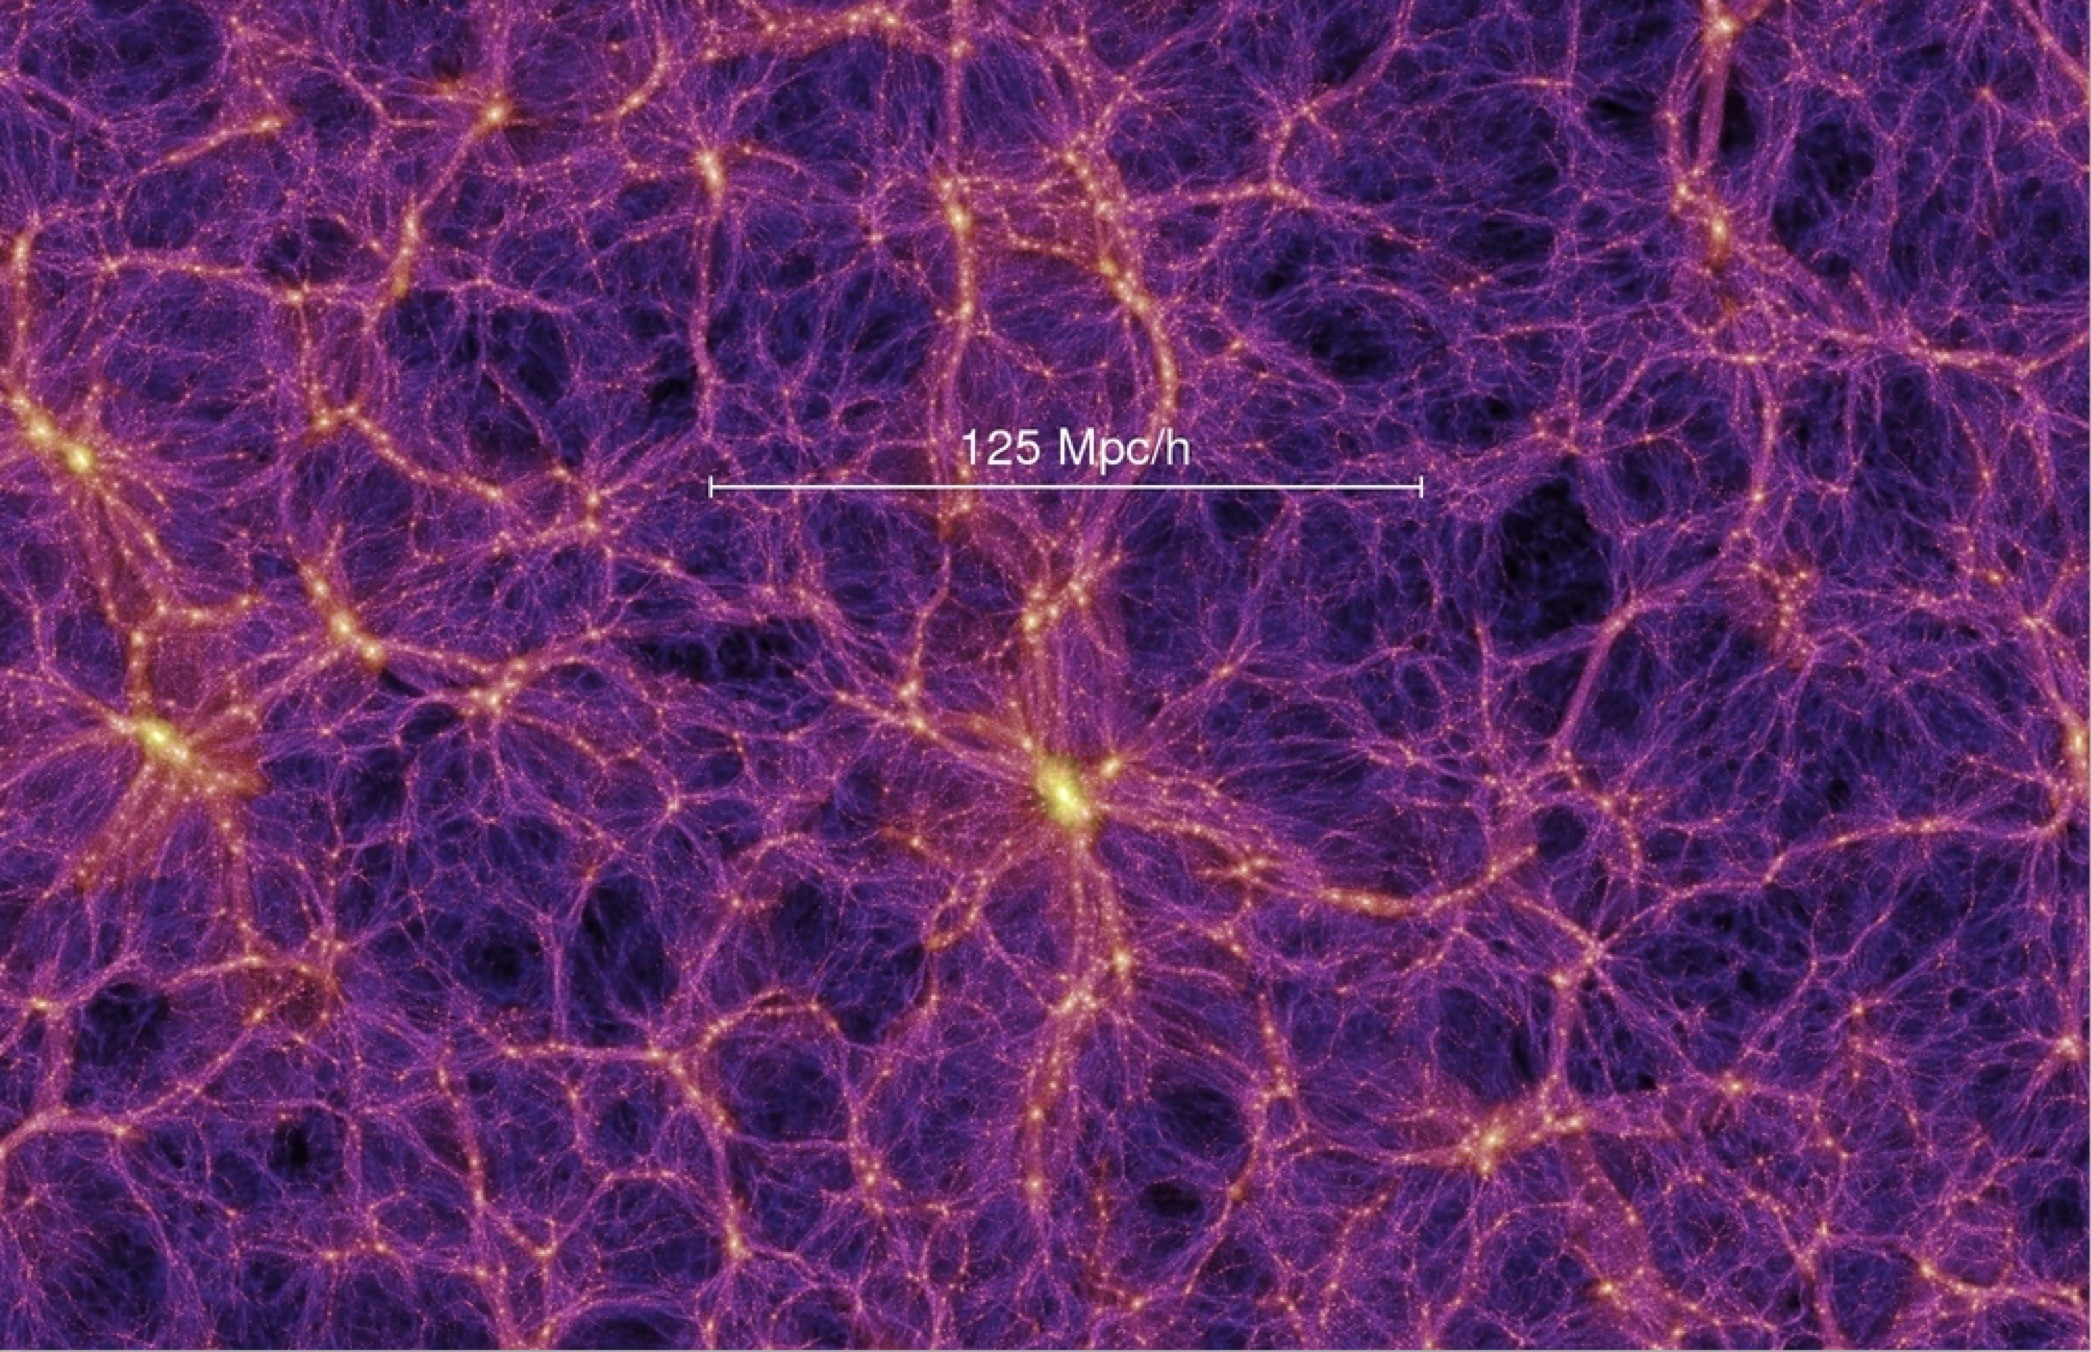
\includegraphics[width=.5\linewidth]{photo/1}
	\caption{Крупномасштабная структура Вселенной}
	\label{fig:figure1}
\end{figure}
\begin{figure}[h!]
	\centering
	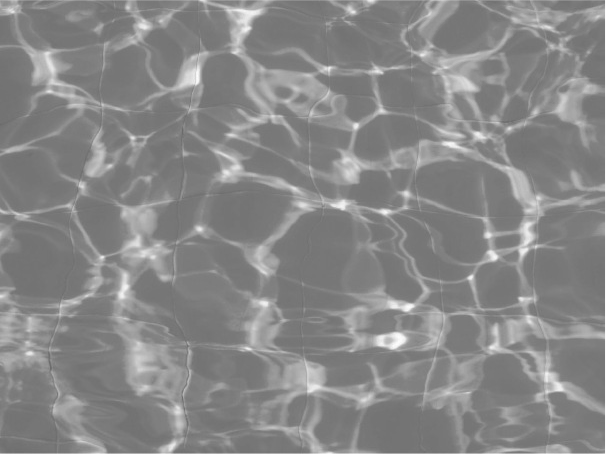
\includegraphics[width=.5\linewidth]{photo/2}
	\caption{Система каустик на дне бассейна}
	\label{fig:figure2}
\end{figure}
В заключение отметим, что результаты динамического моделирования в рамках приближения слипания можно посмотреть на YouTube (\textbf{The Sticky Geometry of the Cosmic Web, version 2.01})

\url{https://www.youtube.com/watch?v=wI12X2zczqI}

Результаты прямого численного моделирования (N-body simulation) можно также  посмотреть на YouTube.

Двухмерный случай:

\url{https://www.youtube.com/watch?v=nHvcqV92oqY}

\url{https://www.youtube.com/watch?v=74IsySs3RGU}

Трехмерный случай

\url{https://www.youtube.com/watch?v=eDGtFRj4xXc}


\newpage
\section{Гидродинамика идеальной жидкости}

В  данном разделе мы рассмотрим законы движения и равновесия идеальной жидкости, то есть жидкости в которой не учитывается внутреннее трение, и следовательно, нет перехода механической энергии в тепловую. Будем также пренебрегать теплообменом между  различными объемами жидкости.

Это означает, что все процессы протекают при постоянной энтропии, а состояние жидкости характеризуется одной скалярной величиной --  давлением $p$. Это, конечно, идеализация, которая приводит к ряду парадоксальных результатов (например, парадокс  Даламбера-Эйлера --  сила сопротивления при равномерном движении тела в жидкости равна нулю). Тем не менее, без этой идеализации невозможно дальнейшее изучение реальных ситуаций.

\subsection{Основные уравнения гидродинамики идеальной жидкости}
Прежде чем перейти к выводу уравнений, рассмотрим два альтернативных способа описания движения жидкости. Оба они были предложены Леонардом Эйлером, но один из них носит имя Лагранжа.

\index{Описание!Лагранжа}
\paragraph{Лагранжево описание.} В основу этого способа положено описание движения отдельных <<жидких частиц>>. При этом все величины, в том числе и  координаты частиц жидкости определяются как функции времени $t$  и некоторых переменных $\xi_k (k=1,2,3)$, идентифицирующих определенную частицу (<<метки>> частиц):
\begin{align*}
	x_i =x_i(\xi_k,t), \quad
	P =P(\xi_k,t), \quad
	\rho = \rho(\xi_k,t), \quad \ldots 
\end{align*}
В качестве переменных $\xi_k$ обычно используют начальные координаты частиц жидкости
\begin{align*}
	% t &=t_0 \\
	\xi_i = x_i(\xi_k, t_0)
\end{align*}

Таким образом, при лагранжевом описании мы следим за определёнными частицами жидкости и смотрим, как изменяются во времени их координаты,  скорости, ускорения, а также давление, температура, плотность в их окрестности.

При этом скорости $\vec{v}$ и ускорения $\vec{a}$ частиц вычисляются по формулам
\begin{align*}
	v_{i} =\frac{\partial x_{i}}{\partial t}, \quad
	a_{i} =\frac{\partial^{2} x_{i}}{\partial t^{2}} 
\end{align*}
Здесь $ \vec{v}\left(\xi_{k}, t\right) $ - скорость частицы в момент времени $t$ имела координаты $\xi_1,\xi_2,\xi_3$.

Отметим, что такому описанию соответствует способ исследования реки с помощью геофизических буев с нулевой плавучестью (см. рис. \ref{fig:figure3}).
\begin{figure}[H]
	\centering
	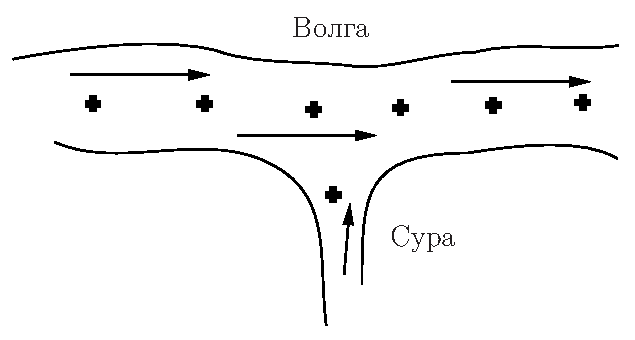
\includegraphics[scale=1]{photo/3.pdf}
	\caption{Схематичная картина Лагранжева и Эйлерова описания}%. \ding{58} - якорь.}
	\label{fig:figure3}
\end{figure}

\index{Описание!Эйлера}
\paragraph{Эйлерово описание.} В этом случае неподвижное пространство заполнено движущейся жидкостью. Движение жидкости будет определено, если все величины, характеризующие жидкость (скорость движения, давление, плотность, температура и т.д.) \textit{будут определены}.
Это означает, что мы можем проследить, как изменяются эти величины от точки к точке:
\begin{align*} 
	\vec{v} =\vec{v}(\vec{x}, t), \quad
	T = T(\vec{x}, t)
\end{align*}
% Система заякоренных буев. 
В Эйлеровом описании мы не знаем, что делается с отдельной частицей. 

При этом частные производные от скорости не являются ускорением. Так, если течение стационарно и частная производная по времени  равна нулю, частицы в данной точке могут иметь ускорение. Пример -- водопад.

Найдем ускорение частицы. За время $ \Delta t $ частица, находящаяся в момент времени $t$ в точке с координатами $ x_{k} $, переместится в точку $ x_{k}=x_{k}+\Delta x_{k} $. Тогда для $i$-ой компоненты ускорения имеем
\begin{align*} 
\lim _{\Delta t \rightarrow 0} \frac{\Delta x_{k}}{\Delta t} &=\frac{\partial x_{k}}{\partial t}=v_{k} 
\end{align*}
\begin{align*}
a_{i} &=\lim _{\Delta t \rightarrow 0} \frac{v_{i}\left(x_{k}+\Delta x_{k}, t+\Delta t\right)-v_{i}\left(x_{k}, t\right)}{\Delta t} = \\
&=\lim _{\Delta t \rightarrow 0}\frac{\left[v_{i}\left(x_{k}, t\right)+\frac{\partial v_{i}}{\partial x_{k}} \Delta x_{k}+\frac{\partial v_{i}}{\partial t}\Delta t-v_{i}\left(x_{k}, t\right)\right]}{\Delta t} =\frac{\partial v_{i}}{\partial x_{k}} v_{k}+\frac{\partial v_{i}}{\partial t} \\
\end{align*}
Таким образом 
\begin{align*} 
a_{i} =\frac{\partial v_{i}}{\partial t}+v_{k} \frac{\partial v_{i}}{\partial t}=\left(\pdv{t}+v_{k} \pdv{t}\right) v_{i}
\end{align*}
Или в векторной форме
\begin{equation}
	\vec{a} =\frac{\partial \vec{v}}{\partial t}+(\vec{v}\,\nabla) \vec{v}=\left(\pdv{t}+(\vec{v}\,\nabla)\right) \vec{v}
\end{equation}

Аналогично находятся и производные от любой другой величины. Эта производная носит название \textit{субстанциональной производной}:
\index{Производная!субстанциональная}
\index{Производная!локальная}
\begin{align*} 
\dv{t}=\pdv{t}+(\vec{v}\,\nabla)
\end{align*}

Первое слагаемое здесь -- \textit{локальная производная}.


\subsection{Связь Лагранжева и Эйлерова описаний}
Пусть нам известно Эйлерово поле скорости $ \vec{v}=\vec{v}\qty(\vec{x}, t) $. Чтобы найти, как двигаются Лагранжевы частицы $ \vec{x}\qty(t, \vec{\xi}\,) $, нам нужно решить уравнение
\begin{align*} 
\dv{\vec{x}}{t}=\vec{v}\qty(\vec{x}, t), \qquad
\vec{x}\qty(t=0, \vec{\xi}\,)=\vec{\xi}
\end{align*}
Как найти эйлерово поле скорости? Если нам известно поведение лагранжевых частиц $ \vec{x}(t, \vec{\xi}\,) $, то вначале нам нужно решить уравнение 
\begin{align*} 
\vec{x}=\vec{x}\qty(t, \vec{\xi}\,)
\end{align*}
Решение этого уравнения $\vec{\xi}=\vec{\xi}\qty(\vec{x}, t)$
позволяет найти Лагранжеву частицу, которая в момент времени $t$ попала в точку $x$. Отсюда в Эйлеровом представлении
\begin{align*} 
\vec{v}(\vec{x}, t)=\vec{v}\qty(t, \vec{\xi}(\vec{x}, t))
\end{align*}




\index{Уравнение!непрерывности}
\index{Закон!сохранения массы}
\subsection{Уравнение непрерывности и закон сохранения массы}
Пусть имеется некоторый объем пространства $V$, заполненный движущейся  жидкостью. Количество жидкости (масса) в этом объеме:
\begin{align*} 
m=\int\limits_{V} \rho\dd{V},
\end{align*}
где $\rho$ - плотность жидкости. Жидкость может притекать и вытекать из объема. Введем элемент поверхности $ \dd\sigma $ и вектор $ \dd \vec{\sigma}=\dd\sigma \vec{n} $, направленный по внешней нормали к поверхности. 
\begin{figure}[H]
	\vspace{-10pt}
	\centering
	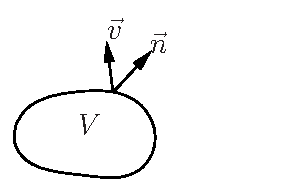
\includegraphics[scale=1]{photo/4.pdf}
	\caption{Объем, скорость и нормаль к поверхности}
	\label{fig:figure4}
\end{figure}
Поток через элемент поверхности определяется скалярным произведением:
\begin{align*}
\oint\limits_{S} \rho \vec{v}\, \dd\vec{\sigma}=\int\limits_{V} \Div(\rho \vec{v}\,)\dd{V}
\end{align*}
Уравнение баланса имеет вид: 
\begin{align*} 
\pdv{t} \int\limits_{V} \rho\dd{V}=-\oint\limits_{S} \rho \vec{v} \dd\vec{\sigma}
\end{align*}
Это интегральный закон сохранения массы. Если на поверхности скорость равна нулю, то масса сохраняется.

Используя формулу Остроградского-Гаусса
\begin{align*} 
\oint\limits_{S} \rho \vec{v}\, \dd \vec{\sigma}=\int\limits_{V} \Div (\rho \vec{v}\,)\dd{V}
\end{align*}
получим 
\begin{align*} 
\int\limits_{V}\left[\frac{\partial \rho}{\partial t}+\Div(\rho \vec{v}\,)\right]\dd{V}=0
\end{align*}

Так как объем произвольный, то мы получаем дифференциальный закон сохранения
\begin{align*} 
\frac{\partial \rho}{\partial t}+\Div(\rho \vec{v}\,)=0
\end{align*}

Вектор $ \vec{j}=\rho \vec{v} $ - плотность потока массы. Используя формулу векторного анализа
\begin{equation}
	\nabla\qty[a \vec{b}]=\nabla a \vec{b}+a \nabla \vec{b},
\end{equation}
перепишем закон сохранения массы в виде:
\begin{align*} 
\frac{\partial \rho}{\partial t}+(\vec{v}\,\nabla) \rho+\rho \Div(\vec{v}\,)=0 \\
\frac{\dd \rho}{\dd t}=-\rho \Div(\vec{v}\,)
\end{align*}

\textbf{Несжимаемая жидкость - плотность частицы вдоль траектории  не меняется.}
\begin{align*} 
\frac{\dd \rho}{\dd t}=0
\end{align*}
Это означает, что поле скорости соленоидально: $\Div\vec{v}=0$.

\index{Уравнение!Эйлера}
\subsection{Уравнение Эйлера}
Это уравнение описывает движение идеальной жидкости и является аналогом {2 закона Ньютона}) классической механики. Запишем второй закон Ньютона для жидкого элемента:
\begin{align*}
\rho\dd{V} \frac{\dd \vec{v}}{\dd t} =\vec{F_{S}}+\vec{F}, \qquad
\vec { F } = \rho \vec { f }
\end{align*}
Здесь $\vec{F}$ --  объемная сила, действующая на элемент $\dd V$, $\vec{f}$ -- сила, отнесенная к единице массы (плотность силы), для силы тяжести $\vec{f}=\vec{g}$, где $g$ -- ускорение свободного падения.

$\vec{F}_s$ -- сила, действующая на элемент объема со стороны окружающей среды.  В идеальной среде силы трения нет, и единственная сила определяется только силами давления. На элемент поверхности $\dd\sigma$ действует сила $ p \dd{\vec{\sigma}} $ и результирующая сила равна:
\begin{align*}
\vec { F } _ { S } = - \oint \limits_ { S } p \dd{\vec{\sigma}} = - \int \limits_ { V } \nabla p\dd{V} \approx - \nabla p\dd{V}
\end{align*}
В результате получаем \textit{уравнение Эйлера}:
\begin{align*}
\dv{\vec{v}}{t} = - \frac { \nabla p } { \rho } + \vec { f }\,
\frac { \partial \vec { v } } { \partial t } + ( \vec{v}\,\nabla ) \vec { v } 
\end{align*}
\begin{equation}
\dv{\vec{v}}{t}=	- \frac { \nabla p } { \rho } + \vec { f }
\end{equation}

Здесь мы учли, что в уравнение Ньютона входит полная производная. У нас  5 неизвестных -- 3 компоненты скорости, давление и плотность. А есть только 4 уравнения: 3 уравнения Эйлера для трех компонент и уравнение непрерывности.

Нужно еще одно уравнение -- уравнение состояния, связывающее давление, плотность и энтропию $S$: 
\begin{equation}
	p = p(\rho,S)
\end{equation}
и уравнение для энтропии. Для изоэнтропической жидкости 
\begin{equation}
	\frac {\dd{S} } { \dd t } = \frac { \partial S } { \partial t } + \vec{v}\,\nabla S = 0
\end{equation}

Если в начальный момент времени энтропия была одинакова во всем пространстве, то она не будет меняться с течением времени и уравнение состояние принимает вид: $ p = p ( \rho ) $.

В идеальном газе уравнение адиабаты имеет вид \textit{уравнения Пуассона}:
\index{Уравнение!Пуассона}
\begin{align*}
p = p_0 \left( \frac{\rho}{\rho_0} \right) ^ { \gamma }, \qq{где}
\gamma = \frac{c_p}{c_v}
\end{align*}
для идеального газа $\gamma = \frac{i+2}{i}$, где $i$ - количество степеней свободы.


Для жидкостей дело хуже. В разных диапазонах давления имеют разные уравнения состояния. Эмпирическая формула для давления $p$, измеряемого в атмосферах: 
\begin{align*}
\frac { p + B } { 1 + B } = \left( \frac { \rho } { \rho_0 } \right) ^ { \gamma }
\end{align*}
где $B=3000\text{ атм}$, $\gamma = 7$, давление до $10^5$ атмосфер.

Итак, \textbf{система уравнений для идеальной жидкости} принимает вид:
\begin{align*}
& \frac { \partial \vec{v} } { \partial t } + ( \vec{v}\,\nabla ) \vec{v} = - \frac { \nabla p } { \rho } + \vec { g } \\
& \frac { \partial \rho } { \partial t } + \Div ( \rho \vec{v} ) = 0 \\
& p = p ( \rho )
\end{align*}

\index{Закон!сохранения энергии}
\subsection{Закон сохранения энергии идеальной жидкости}

Энергия единицы объема складывается из кинетической энергии и  внутренней энергии:
\begin{align*}
E = \frac { 1 } { 2 } \rho v ^ { 2 } + \rho \varepsilon
\end{align*}
Закон сохранения энергии в интегральной форме:
\begin{align*}
\pdv{t} \int\limits_{ V } \rho \left( \frac { 1 } { 2 } v ^ { 2 } + \varepsilon \right)\dd{V} = - \oint\limits_{ S } \rho \left( \frac { 1 } { 2 } v ^ { 2 } + \varepsilon \right) \vec{v} \dd{\vec{\sigma}} - \oint \limits_ { S } p \vec{v} \dd{\vec{\sigma}}
\end{align*}

Изменение энергии в объеме происходит за счет притока (оттока) энергии в объеме через границы, а также за счет работы внешних сил давления. 

Из курса термодинамики и общей физики можно вспомнить, что энтальпия равна 
\begin{equation}
	W = \rho \varepsilon + p 	
\end{equation}
Используя понятие энтальпии, получается упростить выражение ЗСЭ в интегральной форме:
\begin{align*}
\pdv{t} \int \limits_{ V } \rho \left( \frac { 1 } { 2 } v ^ { 2 } + \varepsilon \right)\dd{V} = - \oint \limits_{ S }  \left( \frac { 1 } { 2 } \rho v ^ { 2 } + W \right) \vec{v} \dd{\vec{\sigma}}
\end{align*}
По формуле Стокса переходим в правой части от интегрирования по поверхности к интегрированию по объему:
\begin{align*}
\int \limits_{ V } 
\left[ 
	\pdv{t} 
	\qty( \rho \frac{1}{2} v^2 + \rho \varepsilon) + 
	\Div \qty( 
			\frac{1}{2} \rho v^2 + W 
		) \vec{v} 
\right] \dd{V} = 0
\end{align*}

Поскольку объем произвольный, можно перейти к дифференциальной форме закона сохранения энергии:
\begin{align*}
\frac { \partial E } { \partial t } + \Div \vec { N } = 0 , \qq{где}
E = \frac { \rho v ^ { 2 } } { 2 } + \rho \varepsilon, \quad
\vec { N } = \left[ \frac { \rho v ^ { 2 } } { 2 } + \rho \varepsilon + p \right] \vec{v}
\end{align*}
Здесь $E$ -- плотность энергии, $\vec{N}$ -- вектор плотности потока энергии, аналог вектора Пойнтинга в электродинамике\footnote{Введён в 1874 году Умовым.}.

\index{Закон!сохранения импульса}
\subsection{Закон сохранения импульса}
Для единицы объема жидкости импульс равен $ \vec { p } = \rho \vec{v} $. Если закон сохранения энергии мы выводили в интегральной форме, то здесь мы будем стартовать с дифференциальных уравнений. Запишем изменения для $i$-ой компоненты:
\begin{align*}
\pdv{t} \big( \rho v _ { i } \big) = \rho \frac { \partial v _ { i } } { \partial t } + v _ { i } \frac { \partial \rho } { \partial t }
\end{align*}
Запишем уравнение Эйлера и уравнение непрерывности по компонентам:
\begin{align*}
\frac { \partial v _ { i } } { \partial t } + \sum _ { k = 1 } ^ { 3 } v _ { k } \frac { \partial v _ { i } } { \partial x_k } &= - \frac { 1 } { \rho } \frac { \partial p } { \partial x _ { i } } + f _ { i } \\
\frac { \partial \rho } { \partial t } + \sum _ { k = 1 } ^ { 3 } \frac { \partial \left( \rho v _ { k } \right) } { \partial x _ { k } } &= 0
\end{align*}
В результате для изменения компоненты импульса имеем:
\begin{align*}
\pdv{t} \big( \rho v _ { i } \big) = - \frac { \partial } { \partial x _ { k } } \left( p \delta _ { i k } + \rho v _ { i } v _ { k } \right) + \rho f _ { i }
\end{align*}
Здесь по индексу $k$ идет суммирование. Хочется привести это уравнение к дивергентной форме, чтобы получить закон сохранения. Учтем:
\begin{align*}
\rho v _ { k } \frac { \partial v _ { i } } { \partial x _ { k } } + v _ { i } \frac { \partial \left( \rho v _ { k } \right) } { \partial x _ { k } } = \frac { \partial \left( \rho v _ { i } v _ { k } \right) } { \partial x _ { k } }
\end{align*}
Внешние силы приводят к изменению импульса. Нужно что-то придумать с давлением:
\begin{align*}
\frac { \partial p } { \partial x _ { i } } = \frac { \partial \left( \delta _ { i k } p \right) } { \partial x _ { k } }
\end{align*}
Здесь $ \delta _ { i k } = 1 , i = k ; \delta _ { i k } = 0 , i \neq k $ - символ Кронекера.

В результате получим:
\begin{align*}
\pdv{t} \left( \rho v _ { i } \right) = - \frac { \partial } { \partial x _ { k } } \left( p \delta _ { i k } + \rho v _ { i } v _ { k } \right) + \rho f _ { i }
\end{align*}

Введем тензор плотности потока импульса: $ \Pi _ { i k } = p \delta _ { i k } + \rho v _ { i } v _ { k } $. Тогда закон сохранения импульса запишется как:
\begin{align*}
\pdv{t} \left( \rho v _ { i } \right) = - \frac { \partial \Pi _ { i k } } { \partial x _ { k } } + \rho f _ { i }
\end{align*}

Проинтегрируем последнее равенство по объему:
\begin{align*}
\pdv{t} \int \limits_{ V } \rho v _ { i }\dd{V} = - \int \limits_{ V } \frac { \partial \Pi _ { i k } } { \partial x _ { k } }\dd{V} + \int \limits_{ V } \rho f _ { i }\dd{V}
\end{align*}
Используя теорему Остроградского-Гаусса для тензора получаем:
\begin{align*}
\pdv{t} \int \limits_ { V } \rho v _ { i }\dd{V} = - \oint \limits_ { S } \Pi _ { i k } n _ { k } \dd \sigma + \int \limits_ { V } \rho f _ { i }\dd{V}
\end{align*}
Таким образом, изменение импульса в объеме $V$ связано с потоком импульса через поверхность $S$. Векторная же форма закона сохранения импульса имеет вид:
\begin{align*}
\pdv{t} \int \limits_ { V } \rho  \vec{v}\dd{V}  = - \oint \limits_ { S } \qty[\vphantom{\int} p \vec { n } + \rho \vec{v} ( \vec{v} \vec{n} ) ]\dd\sigma
\end{align*}
Здесь $\vec{n}$ - внешняя нормаль.

\paragraph{Следствие.} Как использовать закон сохранения импульса для нахождения силы действия потока на тело? Если движение стационарно:
\begin{align*}
\oint\limits_{ S } \left[\vphantom{\int} p n _ { i } + \rho v _ { i } v _ { k } n _ { k } \right] \dd \sigma = 0
\end{align*}
Отсюда для силы действия потока на тело имеем:
\begin{align*}
F _ { i } = - \oint \limits_ { S } p n _ { i } \dd \sigma = \oint \limits_ { S } \rho v _ { i } v _ { k } n _ { k } \dd \sigma
\end{align*}
Пример -- изогнутая трубка (душ).
% \begin{align*}
% \pdv{t} \int \limits_ { V } \rho  \vec{v}\dd{V}  = - \oint \limits_ { S } \qty[\vphantom{\int} p \vec { n } + \rho \vec{v} ( \vec{v} \vec{n} ) ]d \sigma
% \end{align*}
\begin{figure}[H]
	\centering
	\includegraphics[width=0.6\textwidth]{example-image-a}
	\caption{Картинка изогнутой трубки}
	\label{fig:figure5}
\end{figure}
В одно сечение жидкость втекает, а из другого вытекает.


\subsection{Гидростатика}
Рассмотрим простейший случай, когда скорость жидкости равна нулю. Из исходной системы уравнений 
\begin{align*}
& \frac { \partial \vec{v} } { \partial t } + ( \vec{v}\,\nabla ) \vec{v} = - \frac { \nabla p } { \rho } + \vec { f } \\
& \frac { \partial \rho } { \partial t } + \Div ( \rho \vec{v} ) = 0 \\
& p = p ( \rho )
\end{align*}
в статическом случае следует
\begin{align*}
\nabla p = \rho \vec { f }, \quad 
p = p ( \rho )
\end{align*}

Пусть внешняя сила потенциальна:
\begin{align*}
& \vec { f } = - \nabla u \\
& \nabla p = - \rho \nabla u,
\end{align*}
то есть градиенты давления и сила параллельны.

При какой зависимости плотности от координаты последнее уравнение имеет решение? Применим к последнему уравнению операцию ротора:
\begin{align*}
&\Rot( \nabla p ) = 0 \\
&\Rot( - \rho \nabla u ) = - \rho\Rot( \nabla p ) - [ \nabla p \times \nabla \rho ] \\ 
& [ \nabla p \times \nabla \rho ] = 0
\end{align*}
Таким образом,  вектора градиентов плотности $\rho$ и потенциала $u$ должны быть параллельны.

Часто встречаются задачи на \textit{распределение давления в поле тяжести}. Запишем уравнения гидростатики в этом случае:
\begin{align*}
\nabla p = \rho \vec { g }, \quad p = p ( \rho ),
\end{align*}
то есть в поле тяжести стационарное решение существует, если плотность зависит от высоты.

Рассмотрим некоторые примеры задач гидростатики.

\paragraph{Жидкость в поле тяжести.} Попросту говоря, простой жизненный пример -- вода в земных условиях.
Плотность постоянна. Ось $z$ направлена вниз.
	\begin{align*}
	& \frac { \dd p } { \dd z } = \rho_0 g \\
	& p = p_a + \rho_0 g z
	\end{align*}
	Давление увеличивается на 1 атмосферу на 10 метрах.

\paragraph{Изотермическая атмосфера.} Под ней понимается идеальный газ с постоянной температурой $T$. Ускорение можно считать постоянным. Ось $z$ направлена вверх.
\begin{align*}
	\frac { \dd p } { \dd z } = - \rho ( z ) g, \quad
	p = \frac { R } { \mu } \frac { m } { V } T = \frac { R } { \mu } \rho T
\end{align*}
Здесь $R$ - универсальная газовая постоянная. $\mu$ - молярная масса газа.
\begin{gather}
	\frac { R T } { \mu } \frac { \dd \rho(z) } { \dd z } = - \rho ( z ) g
\end{gather}
Простое интегрирование даст ответ:
\begin{gather}
	\rho = \rho_0 \exp ( - z / h ) , p = p_0 \exp ( - z / h ), \qq{где}
	h = \frac { R T } { \mu g }
\end{gather}
Здесь $h$ - высота атмосферы, величина порядка 8 км, поэтому изменением силы тяжести можно пренебречь.

\index{Закон!Архимеда}
\paragraph{Закон Архимеда.} На тело, погруженное в жидкость,  со стороны жидкости действует выталкивающая сила, равная весу жидкости, вытесненную этим телом.
\begin{align*}
\nabla p = \rho \vec { g }
\end{align*}
Сила со стороны жидкости на элемент поверхности $ \dd \vec { F } = - p \vec { n }\dd{S} $. Здесь $\vec{n}$ - внешняя нормаль. Тогда сила Архимеда равна:
\begin{align*}
& \vec { F }_ { A }  = - \oint \limits_ { S } p \vec{n}\dd{S} = - \int \limits_ { V } \nabla p\dd{V} = - \int \limits_ { V } \rho \vec { g }\dd{V}=\vec{P}\\
& \int _ { V } \rho \vec { g }\dd{V}  \approx \rho V \vec { g } \\
% & & \vec { F }_ { A } = - \vec { p }
\end{align*}
Здесь $\vec{P}$ -- вес вытесненнной жидкости. Причем и плотность, и ускорение \textit{не обязательно постоянны!}


\subsection{Гидростатическое равновесие. Частота Брента — Вяйсяля}
\index{Равновесие!гидростатическое}
Выясним условия, при  которых состояние равновесия стратифицированной жидкости в поле тяжести будет устойчивым. Будем считать, что плотность зависит от глубины произвольным образом $\rho=\rho(z)$. Ось $z$ направлена вниз. 

\begin{figure}[H]
	\centering
	\includegraphics[width=0.6\textwidth]{example-image-a}
	\caption{Действие силы Архимеда на возмущенный элемент}
	\label{fig:arch}
\end{figure}
% Если можно вставить рисунок с двумя положениями выделенного элемента жидкости и с силами Архимеда и тяжести, причем на погруженном элементе сила Архимеда больше силы тяжести

Рассмотрим элементарный элемент жидкости, который находился в равновесии на глубине $z$, потом возмущается перемещением на глубину $z+x$.

На этот элемент жидкости действуют две силы: сила тяжести и сила Архимеда, и в равновесии они равны  по величине:
\begin{align*}
F _ { g } ( z ) &= g \rho ( z ) V_0 \\
F _ { A } ( z ) &= - F _ { g } ( z ) = - g \rho ( z ) V_0
\end{align*}

Пусть данный объем смещается по вертикали на расстояние $x$. Масса сохраняется и сила тяжести не меняется.  Пусть \textit{жидкость несжимаема}, тогда объем не меняется. А сила Архимеда изменяется, так как плотность вокруг частицы изменилась. Тогда уравнение  Ньютона для объема запишется как:
\begin{align*}
& m \frac { \dd ^ { 2 } x } { \dd t ^ { 2 } } = g \rho ( z ) V_0 - g \rho ( z + x ) V_0 \\
& m = \rho ( z ) V_0
\end{align*}

Разлагая плотность в ряд, и ограничиваясь линейными членами, получаем:
\begin{align*}
\frac { \dd ^ { 2 } x } { \dd t ^ { 2 } } = - \frac { g } { \rho } \frac { \dd \rho } { \dd z } x
\end{align*}
Это уравнение гармонического осциллятора:
\index{Частота!Брента-Вяйсаля}
\begin{align*}
& \frac { \dd ^ { 2 } x } { \dd t ^ { 2 } } + N ^ { 2 } x = 0 \\
& N ^ { 2 } = \frac { g } { \rho } \frac { \dd \rho } { \dd z } \sim \frac { g } { L }
\end{align*}
Здесь $\displaystyle N = \left( \frac { g } { \rho } \frac { \dd \rho } { \dd z } \right) ^ { 1 / 2 } $ -- \textit{частота Брента-Вяйсаля}.
\begin{enumerate}
	\item {\textit{Устойчивость жидкости} наблюдается при $ N ^ { 2 } > 0 , \frac { \dd \rho } { \dd z } > 0$. Элемент совершает колебания с частотой $N$.}
	\item {\textit{Неустойчивость жидкости} наблюдается при $ N ^ { 2 } < 0 $. Элемент падает вниз или стремится всплыть.}
\end{enumerate}


\subsection{Уравнение Бернулли}
\index{Уравнение!Бернулли}
% Получим альтернативную запись уравнения Эйлера в форме Громэка-Лэмба:
Запишем уравнение Эйлера. Внешней силой здесь является сила тяжести, которую можно записать через градиент (так как орт оси $z$ равен $\nabla z$): 
\begin{align*}
\frac { \partial \vec{v} } { \partial t } + ( \vec{v}\,\nabla ) \vec{v} = - \frac { \nabla p } { \rho } + \vec { g }, \qquad
\vec { g } = g \nabla z
\end{align*}
Ось $z$ направлена вниз. Учтем два равенства: из курса векторного анализа
\begin{equation}
	(\vec {v}\, \nabla ) \vec{v} = \frac12\Grad\qty(v^2) - \qty[ \vec{v} , [\nabla , \vec{v}\,]]
\end{equation}
 и из курса термодинамики (для равновесных обратимых изобарических процессов):
\begin{align*}
\frac { \nabla p } { \rho } = \nabla W 
\end{align*}
Заметим, что если плотность среды постоянна, то $\frac{\nabla p}{\rho}=\nabla\qty(\frac{p}{\rho})$.

\index{Уравнение!Эйлера!форма Громэко-Лэмба}
Получаем уравнение Эйлера \textit{в форме Громэко-Лэмба}:
\begin{align*}
\frac { \partial \vec{v} } { \partial t } +\Grad \left( \frac { v ^ { 2 } } { 2 } + W - g z \right) = [ \vec{v} , \Rot \vec{v}\,]
\end{align*}

Рассмотрим частные случаи, получающиеся из этого уравнения при некоторых условиях.

\subsubsection{Случай стационарного движения}
\index{Движение!стационарное}
В стационарном случае ($\vec{v}=\const$) можно выделить два подслучая: безвихревого и вихревого движения. Рассмотрим их подробнее.

\paragraph{Безвихревое движение.}
\index{Движение!стационарное!безвихревое}
Движение потенциальное, $\Rot \vec{v}=0$. 		Тогда из уравнения Громэко-Лэмба имеем
\begin{align*}
&\Grad \left( \frac { v ^ { 2 } } { 2 } + W - g z \right) = 0 \\
& \frac { v ^ { 2 } } { 2 } + W - g z = \const
\end{align*}
Заметьте, константа в этом случае \textit{сохраняется во всем пространстве.} Если жидкость несжимаема и однородна, то:
\begin{align*}
\frac { v ^ { 2 } } { 2 } + \frac { p } { \rho } - g z = \const
\end{align*}
Это уравнение Бернулли для стационарного \textbf{потенциального} движения однородной несжимаемой жидкости.

\paragraph{Вихревое движение.}
\index{Движение!стационарное!вихревое}
Теперь $\Rot \vec{v} \neq 0$. 
Введем понятие линии тока. 

\textbf{Линия тока} - это линия, касательные к которой в данный момент времени и в каждой точке совпадают с вектором скорости $\vec{v}$. 
\begin{figure}[H]
	\centering
	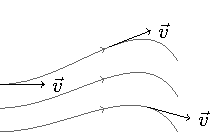
\includegraphics[scale=1.5]{img/line}
	\caption{Линии тока}
	\label{fig:figure6}
\end{figure}
Линии тока определяются системой дифференциальных уравнений:
\begin{align*}
\frac { \dd x } { \dd v _ { x } } = \frac { \dd y } { \dd v _ { y } } = \frac { \dd z } { \dd v _ { z } }
\end{align*}
Умножим скалярно уравнение Эйлера (в форме Громэко-Лэмба) на вектор скорости, то есть, спроектируем его на линии тока:
\begin{align*}
	\vec {v}\cdot[ \vec{v} , \Rot \vec{v}\,]=0, \qq{так как}
	\vec {v} \perp [ \vec{v} , \Rot \vec{v}\,]
\end{align*}
% \textcolor{red}{Будем рассматривать случай несжимаемой жидкости, тогда $W=\frac{p}{\rho}$.}
В таком случае уравнение Эйлера в проекции на линию тока сведется в виду 
\begin{equation}
	\vec{v}\cdot \Grad\qty(\frac{v^2}{2}+W-gz)=0
\end{equation}
Но такое произведение можно трактовать как производную по направлению:
\begin{align*}
	\vec{v}\,\nabla \qty(\frac{v^2}{2}+W-gz) = \dv{l}\qty(\frac{v^2}{2}+W-gz) = 0
\end{align*}
отсюда получаем по форме тот же закон сохранения, что и для безвихревого движения:
\begin{align*}
	\frac { v ^ { 2 } } { 2 } + W - g z = \const
\end{align*}
Но здесь константа сохраняется только вдоль линии тока, и \textit{для разных линий тока константы разные!}

\subsubsection{Случай нестационарного невихревого движения}
\index{Движение!нестационарное невихревое}
В этом случае
\begin{align*}
	\frac { \partial \vec{v} } { \partial t } \neq 0, \qquad
	\Rot \vec{v} = 0
\end{align*}
Рассматриваем  потенциальные течения: $ \vec{v} = \nabla \varphi $. Тогда из уравнения Громэко-Лэмба, используя возможность перестановки $\nabla$ и $\pdv{t}$ местами, нетрудно получить закон сохранения
\begin{align*}
\frac { \partial \phi } { \partial t } + \frac { v ^ { 2 } } { 2 } + W - g z = \mathrm { const }
\end{align*}
Этот интеграл движения носит название \textit{интеграла Коши.}

\subsubsection{Энергетический смысл уравнения Бернулли}

Закон Бернулли --  это ничто иное, как следствие законов сохранения массы и энергии вдоль некоторой лучевой трубки через 2 сечения: входящее $S_1$ и выходящее $S_2$ (см. рис. \ref{fig:figure7}).

\textbf{Определение. } Лучевая трубка тока -- это трубка, образованная множеством линий тока, проходящих через некоторый замкнутый контур
\begin{figure}[H]
	\centering
	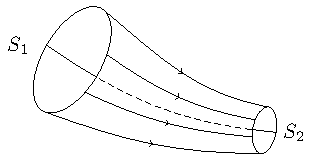
\includegraphics[scale=1.5]{img/trubka}
	\caption{Лучевая трубка}
	\label{fig:figure7}
\end{figure}

Закон сохранения массы заключается в равенстве: сколько втекает, столько и вытекает.
\begin{align*}
m _ { i } = \rho _ { i } S _ { i } v _ { i } \Delta t , \quad i = 1,2
\end{align*}
Изменение энергии за счет вытекания и работы силы тяжести равно работе внешних сил:
\begin{align*}
& A _ { i } = p _ { i } S _ { i } v _ { i } \Delta t \\
& E _ { i } = \frac { v _ { i } ^ { 2 } } { 2 } + u _ { i } + \varepsilon _ { i } \\
& A _ { 1 } - A _ { 2 } = \Delta m \left( E _ { 2 } - E _ { 1 } \right)
\end{align*}
Здесь $u$ и $\varepsilon$ - потенциальная и внутренняя энергия. Рассмотрим случай несжимаемой жидкости. В этом случае внутренняя энергия не меняется, а $ u = - g z $. В результате получим уравнение Бернулли.



Уравнение Бернулли имеет множество приложений.
\paragraph{Трубка Вентури.}
\index{Трубка Вентури}
Знаем сечения, измеряем давления -- находим скорости:
\begin{align*}
& \frac { v _ { 1 } ^ { 2 } } { 2 } + \frac { p _ { 1 } } { \rho } = \frac { v _ { 2 } ^ { 2 } } { 2 } + \frac { p _ { 2 } } { \rho } \\
& S _ { 1 } v _ { 1 } = S _ { 2 } v _ { 2 }
\end{align*}
\begin{figure}[H]
	\centering
	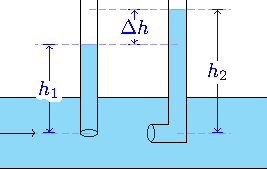
\includegraphics[scale=1.3]{img/pito}
	\caption{Трубка Пито (переделать рисунок)}
	\label{fig:figure8}
\end{figure}


\paragraph{Обтекание двух цилиндров.}
\index{Обтекание!двух цилиндров}
Сближение линий тока, увеличение скорости. Возникает притяжение цилиндров.
\begin{figure}[H]
	\centering
	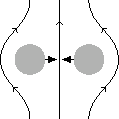
\includegraphics[scale=1.5]{img/2cy}
	\caption{Схематический вид цилиндров}
	\label{fig:figure9}
\end{figure}

\index{Вытекание жидкости}
\paragraph{Вытекание жидкости из сосуда.}
\begin{align*}
& \sigma \ll S \\
& v = \sqrt { 2 g \left( z _ { 1 } - z _ { 2 } \right) }
\end{align*}
\begin{figure}[H]
	\centering
	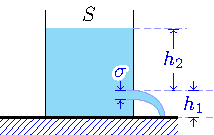
\includegraphics[scale=1.5]{img/vutekanie}
	\caption{Схематичный вид вытекающей жидкости}
	\label{fig:figure10}
\end{figure}

\index{Задача!Прандтля}
\paragraph{Задача Прандтля.} Эта задача описывает косое падение плоской струи на поверхность и так называемы кумулятивные снаряды. Наряду с уравнением Бернулли нужно использовать закон сохранения импульса.
\begin{figure}[H]
	\centering
	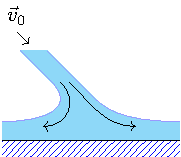
\includegraphics[scale=1.5]{img/prandtl}
	\caption{Наклонное падение струи}
	\label{fig:figure11}
\end{figure}
% \begin{figure}[H]
% 	\centering
% 	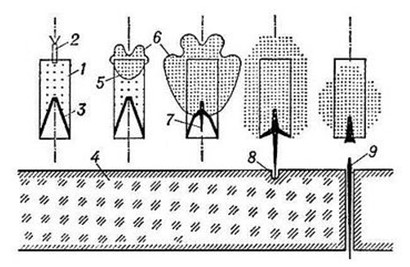
\includegraphics[scale=1]{photo/kommu.jpg}
% 	\caption{Кумулятивные снаряды}
% 	\label{fig:figure12}
% \end{figure}



\subsection{Теорема Томсона. Потенциальные и вихревые движения жидкости}
\index{Теорема!Томсона}

Введём понятие циркуляции скорости -- интеграл, взятый вдоль некоторого замкнутого контура
\begin{align*}
\Gamma = \oint \limits_ { L } \vec{v} \dd{\vec{r}}
\end{align*}
Докажем теорему о сохранении циркуляции скорости -- теорему Томсона (лорда Кельвина):
\textbf{Циркуляция скорости вдоль замкнутого контура, перемещающегося в идеальной жидкости, остается постоянной.}

\begin{figure}[h!]
	\centering
	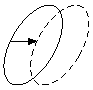
\includegraphics[scale=1.5]{img/2contur}
	\caption{Два контура: начальный и смещенный}
	\label{fig:figure13}
\end{figure}

Выберем замкнутый контур, состоящий из фиксированных частиц (<<жидкий>> контур) и перемещающийся вместе с ними.  Найдем полную производную по времени от этого контура. Происходит изменение как скорости, так и изменение контура во времени
\begin{align*}
\frac{\dd \Gamma}{\dd t}=\frac{d}{\dd t} \oint\limits_{L} \vec{v} \dd \vec{r}=\oint\limits_{L} \frac{\dd \vec{v}}{\dd t} \dd \vec{r}+\oint\limits_L \vec{v}\, d\left(\frac{\dd \vec{r}}{\dd t}\right)
\end{align*}
%
Используем определение скорости и уравнение Эйлера
\begin{align*}
\frac { \dd \vec{v}  } { \dd t } = - \frac { \nabla p } { \rho } + \vec { f }
\end{align*}
%
Пусть внешняя сила потенциальна, а процесс адиабатический:
\begin{align*}
{ \vec { f } = - \nabla u }, \quad
{ \frac { \nabla p } { \rho } = \nabla W }
\end{align*}
Здесь $W$ -- энтальпия.  Учтем, что $ ( \nabla \phi \dd{\vec{r}}\, ) = \dd \phi $ и окончательно получим
\begin{align*}
\frac { \dd \Gamma } { \dd t } = \oint\limits _ { L } \dd \left( \frac { v ^ { 2 } } { 2 } - W - u \right) = 0 \quad \Rightarrow \quad  \Gamma = \const
\end{align*}

% \begin{itemize}
\paragraph{Следствие 1.} Используем теорему Стокса:
\begin{align*}
\Gamma = \oint \limits_ { L } \vec{v} \dd{\vec{r}} = \int \limits_ { S } \vec { n }\Rot\vec{v}\dd{S}
\end{align*}
% \begin{figure}[h]
% 	\centering
% 	\includegraphics[width=0.6\textwidth]{example-image-c}
% 	\caption{Контур и поверхность, натянутая на этот контур}
% 	\label{fig:figure14}
% \end{figure}

Для потенциальных течений $ \Rot \vec{v} = 0 \Rightarrow \Gamma = 0$: \textit{Циркуляция скорости по {односвязному контуру} в потенциальном течении идеальной жидкости равна нулю.}

\paragraph{Следствие 2.} 	Поток вихря через поверхность, натянутую на  \textit{односвязный контур} в потенциальном течении идеальной жидкости -- величина постоянная:
	\begin{align*}
	\Gamma = \oint \limits_ { L } \vec{v} \dd{\vec{r}} = \int \limits_ { S } \vec { n }  \Rot \vec{v}\dd{S} = \const
	\end{align*}


\paragraph{Следствие 3.} В потенциальном течении не может быть \textit{замкнутых линий тока} (иначе, взяв одну из них в качестве контура, мы получим, что циркуляция вдоль данного контура не равна нулю).

\paragraph{Следствие 4.} В однородной несжимаемой жидкости можно исключить из рассмотрения уравнений движения давление.  Запишем уравнение Эйлера в форме Громэко-Лэмба
\begin{equation}
	\frac { \partial \vec{v} } { \partial t } +\Grad \left( \frac { v ^ { 2 } } { 2 } + W - g z \right) = [ \vec{v} , \Rot \vec{v}\,]
\end{equation}
Возьмем от него ротор и учтем, что ротор от градиента равен нулю ($\Rot\qty(\nabla \qty(\ldots))= 0 $):
\begin{align*}
{ \pdv{t} \Rot \vec{v} = \Rot [ \vec{v} \Rot \vec{v} ] }, \qquad
{\Div \vec{v} = 0 }
\end{align*}
Получили полное описание поля скорости с помощью одного уравнения.


% \subsubsection{}
\paragraph{Основные выводы из теоремы Томсона.} Если в какой-то точке линии тока завихренность отсутствует, то она отсутствует и вдоль этой линии. На первый взгляд, отсюда следует:

\vspace{0.5em}
% На первый взгляд отсюда следует:
% \begin{enumerate}
\textit{Первый вывод.} Стационарное обтекание любого тела набегающим из бесконечности потоком должно быть потенциальным: $\vec{v} = \text { const }, \,\,\Rot\vec{v} = 0$
\vspace{0.5em}

\textit{Второй вывод.} Если движение жидкости потенциально в некоторый момент времени, то оно будет потенциальным и в дальнейшем. В частности, потенциальным должно быть всякое движение, при котором в начальный момент жидкость покоилась. 
\vspace{0.5em}

В реальности, однако, это имеет ограниченную область применимости. Дело в том, что приведенное выше утверждение о сохранении ротора скорости вдоль линии тока неприменимо для линий, проходящих вдоль поверхности твердого тела. Около стенки \textit{нельзя провести односвязный замкнутый контур}. 
\begin{figure}[H]
	\centering
	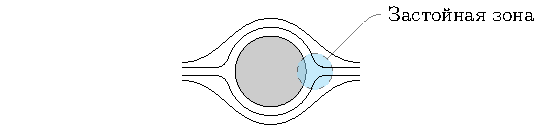
\includegraphics[scale=1.2]{img/tang}
	\caption{Обтекание тела с застойными зонами}
	\label{fig:figure14}
\end{figure}
Уравнения движения идеальной жидкости допускают решения в которых на поверхности твердого тела, обтекаемого жидкостью твердого тела происходит <<отрыв>> струи: линии тока, следовавшие вдоль поверхности, в некотором месте отрываются от него, уходя в глубь жидкости. Возникает застойная область и на границе течение становится непотенциальным (см. рис. \ref{fig:figure14}), возникает поверхность <<тангенциального>> разрыва. Скорость терпит разрыв непрерывности.


При учете таких разрывных решений решение уравнений идеальной жидкости неоднозначно: наряду с непрерывным решением появляется бесконечное множество разрывных решений. При этом разрывные решения не имеют физического смысла, так как тангенциальные разрывы \textbf{абсолютно неустойчивы}, в результате чего движение жидкости становится \textbf{турбулентным}.

Реальное течение безусловно однозначно. Всякая жидкость обладает вязкостью. Малая вязкость практически не проявляется во всем пространстве, но она будет играть определяющую роль в пристеночной области (пограничный слой).

Тем не менее, в ряде случаев это достаточно хорошее приближение.  Например, \textit{хорошо обтекаемые тела}: самолет, автомобиль, корабль -- движение жидкости от потенциального отличатся только в области <<пограничного>> слоя и <<следа>> позади тела.

Кроме того, это приближение работает и в случае \textit{малых нестационарных колебаний}. Рассмотрим его подробнее.


\subsubsection{Нестационарные малые колебания}
\index{Колебания!малые нестационарные}
Рассмотрим слабо колеблющееся тело в жидкости. Пусть $l$ -- линейный размер тела, $a$ -- характерная амплитуда колебаний, $v$ -- скорость колеблющегося тела.
\begin{figure}[H]
	\centering
	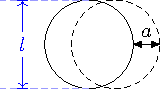
\includegraphics[scale=1.5]{img/sphere}
	\caption{Сфера размером $l$ и сфера, смещённая на $a$.}
	\label{fig:figure15}
\end{figure}
Если $l \gg a$, то движение жидкости вокруг тела потенциально. Покажем это, оценив порядок величины различных членов в уравнении Эйлера (для несжимаемой жидкости, без внешних сил):
\begin{align*}
\frac { \partial \vec{v} } { \partial t } + ( \vec{v}\,\nabla ) \vec{v} = - \nabla W
\end{align*}
Скорость (порядка скорости колеблющегося тела $u$) изменяется на  масштабах $l$. Поэтому производные от скорости по координатам порядка $\sim u/l$. Изменения же скорости во времени определяются частотой колебаний $\sim \omega u$. Тогда
\begin{align*}
\frac{
\left| \cfrac { \partial \vec{v} } { \partial t } \right|} {\left| (\vec{v}\,\nabla ) \vec{v} \right|} \sim \cfrac{\phantom{a}\cfrac { u ^ { 2 } } { a }\phantom{a}} { \cfrac { u ^ { 2 } }{ l } } \sim \frac { l } { a } \gg 1
\end{align*}
Значит, вторым членом можно пренебречь, и тогда уравнение Эйлера принимает вид:
\begin{align*}
\frac { \partial \vec{v} } { \partial t } = - \nabla W
\end{align*}
Возьмем от полученного уравнения ротор. Так как при колебательном движении среднее значение скорости по периоду равно нулю, то $\const=0$:
\begin{align*}
\pdv{t}  \Rot  \vec{v} = 0 , \quad\Rot\vec{v} =  \const  = 0
\end{align*}


Таким образом, \textit{малые нестационарные колебания потенциальны}.


\subsection{Потенциальные течения несжимаемой жидкости}
\index{Течение!потенциальное}
\index{Парадокс Даламбера}
\index{Присоединенная масса}

В идеальной баротропной жидкости в поле потенциальных сил вихри не исчезают и не возникают. Если в начальный момент течение было потенциально, то оно будет потенциальным всегда. В ряде случаев это достаточно хорошее приближение, а уравнения гидродинамики существенно упрощаются. 

Уравнение непрерывности несжимаемой жидкости:
\begin{align*}
\frac { \dd \rho } { \dd t } = 0 ,\quad \Div \vec{v} = 0
\end{align*}
Поле скорости несжимаемой жидкости соленоидально. Уравнение Эйлера для несжимаемой жидкости в форме Громэко-Лэмба:
\begin{align*}
\pdv{\vec{v}}{t} + \Grad\qty(\frac{v^2}{2}+\frac{p}{\rho}-gz) = [\vec{v} \Rot\vec{v}\,]
\end{align*}
Отсюда легко получить следствие из уравнения Эйлера (мы это делали раньше):
\begin{align*}
\pdv{t}\Rot\vec{v} =\Rot[ \vec{v}\Rot\vec{v}  \, ]
\end{align*}
Это означает, что если движение было потенциально в начальный момент времени, то и в дальнейшем оно будет потенциальным. Поэтому можно ввести потенциал поля скорости
\begin{align*}
 &\Rot \vec{v} = 0 , \quad  { \vec{v} =\Grad \varphi } \\  
 &\operatorname { div\, grad } \varphi = \Delta \varphi = 0 
\end{align*}
Таким образом, описание потенциального движения идеальной несжимаемой жидкости описывается уравнением Лапласа:
\begin{align*}
\Delta \varphi = 0 , \quad \vec{v} =\Grad \varphi
\end{align*}
Для решения этого уравнения также необходимы граничные условия.

\textbf{Г.у. непротекания}: нормальная компонента скорости жидкости на поверхности тела должна совпадать с проекцией $v_n=\frac { \partial \varphi } { \partial n }=u_n$ скорости самого тела на эту нормаль. 

\textbf{Г.у. бесконечности}: обычно используют значение потенциала на бесконечности.

% Возникает вопрос: \textbf{как найти давление?} Ответ: из уравнения Бернулли.
Давление теперь можно найти из уравнения Бернулли:
\begin{align*}
& \frac { \partial \varphi } { \partial t } + \frac { v ^ { 2 } } { 2 } + \frac { p } { \rho } + u =  \const  \\
& p = - \left( \frac { \partial \varphi } { \partial t } + \frac { v ^ { 2 } } { 2 } + u \right) +  \const 
\end{align*}
Константа может зависеть от времени. Для стационарного течения:
\begin{align*}
p = - \left( \frac { v ^ { 2 } } { 2 } + u \right) +  \const 
\end{align*}
% \begin{center}
% 	\textbf{======Здесь остановился Максим=======}
% \end{center}
Рассмотрим несколько частных решений уравнения Лапласа, известных в  электростатике.

\paragraph{Сдвиговый поток.} Эта задача аналогична задаче поля плоского конденсатора в электростатике. Все частицы жидкости двигаются с постоянной скоростью
\begin{equation}
    \vec{v}_0 = \{v_x, v_y, v_z\}, \quad
    \vec{r} = \{x,y,z\}
\end{equation}
Потенциал здесь будет
\begin{equation}
    \phi = \qty(\vec{v}_0,\vec{r}\,) = v_x x + v_y y + v_z z
\end{equation}
Очевидно, он удовлетворяет уравнению Лапласа:
\begin{equation}
    \Delta \phi = \pdv[2]{\phi}{x}+ \pdv[2]{\phi}{y} + \pdv[2]{\phi}{z}=0, \quad
    \vec{v} = v_x \vec{i} + v_y \vec{j} + v_z \vec{k}
\end{equation}
\begin{figure}[H]
    \centering
    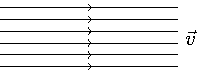
\includegraphics[scale=1.5]{img/sdvig}
    \caption{Параллельные линии тока}
    \label{fig:sdvigovuipotok}
\end{figure}

\paragraph{Монополь.} Эта задача о стоке и истоке массы: потенциал здесь
\begin{equation}
    \phi = \frac{\alpha}{r}, \quad \vec{v} = \Grad \phi = \pdv{\phi}{r} \vec{i}, \quad \vec{v} = -\frac{\alpha}{r^2}  \frac{\vec{r}}{r} = 
    -\frac{\alpha}{r^2} \vec{i}
\end{equation}
Решение сферически симметрично и имеет особенность в точке $r=0$. Заметим, что поток массы через сферу вокруг монополя произвольного радиуса -- величина постоянная:
\begin{equation}
    m = \rho\, 4\pi r^2\, |v| = \rho\cdot 4\pi\alpha
\end{equation}
Знак <<+>> говорит о стоке массы, <<->> -- о истоке.
\begin{figure}[H]
    \centering
    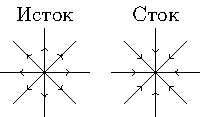
\includegraphics[scale=1.5]{img/stok_istok}
    \caption{Сток и исток массы}
    \label{fig:stokistok}
\end{figure}

\paragraph{Диполь.} Поместив сток и исток рядом, устремим их интенсивность в бесконечность, а расстояние между ними к нулю. Потенциал диполя
\begin{equation}
    \phi = \vec{A} \cdot \Grad \frac{1}{r}
\end{equation}

\subsubsection{Движение сферы в идеальной жидкости}
Пусть сфера радиуса $R$ движется с постоянной скоростью в несжимаемой 
неограниченной жидкости. Течение при этом потенциально, а на бесконечности поставим <<граничное условие>> $v=0$. На поверхности сферы должны быть равны нормальные (относительно поверхности) компоненты скорости сферы и жидкости. При этом систему координат выберем с началом в центре сферы. 

Математическая формулировка такой задачи будет следующей:
\begin{equation}
    \Delta \phi = 0, \quad
    \vec{v} |_{r\to \infty}=0, \quad
    v_r |_{r=R}=v_{\text{сф}_r}|_{r=R}
\end{equation}
Попробуем подобрать решение в виде диполя (сток-исток не подходит):
\begin{equation}
    \phi = \vec{A} \Grad \frac{1}{r} = B \vec{v}_0 \Grad \frac{1}{r}=
    -B \frac{\qty(\vec{v}_0,\vec{r}\,)}{r^3}
\end{equation}
Тогда скорость жидкости
\begin{equation}
    \vec{v} = \Grad \phi = -B \frac{\vec{v}_0}{r^3} +
    3B \frac{(\vec{v}_0,\vec{r}\,)\cdot \vec{r}}{r^5}
\end{equation}
Удовлетворим граничным условиям. Условие равенства нормальных (в нашей системе координат направление нормали -- радиальное):
\begin{equation}
    v_r |_{r=R}= v_{0_r}|_{r=R}
    -\frac{B{v_{0_r}}}{R^3}
    +3\frac{B v_{0_r}}{R^3} = v_{0_r} 
\end{equation}
Отсюда константа $B=\frac{R^3}{2}$, и тогда для потенциала и скорости конечные формулы
\begin{equation}
    \phi = -\frac{1}{2} \frac{R^3}{r^3} \qty(\vec{v}_0,\vec{r}\,), \quad
    \vec{v} = -\frac{1}{2} \frac{R^3}{r^3} \vec{v}_0
    +\frac{1}{2} \frac{R^3}{r^5} (\vec{v}_0,\vec{r}\,)\cdot \vec{r}
\end{equation}
В сферической системе координат
\begin{equation}
    \phi = -\frac{1}{2} \frac{R^3}{r^2} v_0 \cos\theta, \quad
    \vec{v} = \Grad\phi = \pdv{\phi}{r} \vec{I}_r +
    \frac{1}{r} \pdv{\phi}{\theta} \vec{I}_\theta,
\end{equation}
Отсюда радиальная и тангенциальная компоненты скорости соответственно
\begin{equation}
    v_r= \frac{v_0 R^3}{r^3}\cos\theta, \quad
    v_\theta = \frac{v_0 R^3}{2r^3} \sin\theta
\end{equation}

\paragraph{Объединение решений сферы и плоского потока.} В силу линейности уравнения Лапласа, можно легко решить задачу об обтекании сферы постоянным потоком объединением решений плоского потока и диполя (сферы). Для определённости, будем считать что поток набегает на сферу справа. 

При этом математическая формулировка задачи будет
\begin{equation}
    \Delta \phi = 0, \quad
    \pdv{\phi}{r}\bigg|_{r\to \infty} = -v_0 \cos\theta, \quad
    \pdv{\phi}{r}\bigg|_{r=R} = 0
\end{equation}

Решение задачи будут суперпозицией решений задачи сферы и задачи плоского потока:
\begin{equation}
    \phi = -v_0 \cos\theta \qty(1+\frac{1}{2}\frac{R^3}{r^2}), \quad
    v_r = -v_0\cos\theta \qty(1-\frac{R^3}{r^3}),
\end{equation}
\begin{equation}
	v_\theta = v_0\sin\theta \qty(1+\frac{R^3}{2r^3})
\end{equation}
При этом на поверхности сферы
\begin{equation}
    v_r = 0, \quad
    v_\theta = \frac{3}{2}v_0\sin\theta
\end{equation}
В точках $\theta=0,\pi$ скорость $v_\theta=0$, а в точках $\theta=\frac{\pi}{2}, \frac{3\pi}{2}$ скорость $v_\theta=\frac{3}{2}v_0$.

\subsubsection{Парадокс Даламбера-Эйлера.} Найдём давление и силу, 
действующие со стороны потока на неподвижную сферу. Для этого задействуем
 уравнение Бернулли:
\begin{equation}
    p_0 + \frac{\rho v_0^2}{2} = 
    p_s + \frac{\rho v_\theta^2}{2}
\end{equation}
Учитывая, что $v_\theta=\frac{3}{2}v_0\sin\theta$, получим
\begin{equation}
    p_s = p_0 + \frac{\rho v_0^2}{2}\qty(1-\frac{9}{4}\sin^2\theta)
\end{equation}
\begin{figure}[H]
    \centering
    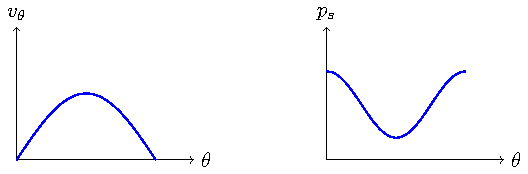
\includegraphics[width=\textwidth]{img/p_vtheta}
    \caption{Графики скорости и давления от угла}
    \label{fig:pandv}
\end{figure}
Давление симметрично относительно миделя (серединной плоскости) сферы. Найдём полную силу со стороны жидкости на сферу:
\begin{equation}
    \vec{F} = - \oint\limits_S p_s \vec{n} \dd{S}
\end{equation}
Можно подставить сюда давление и посчитать силу в лоб. Но намного проще
 заметить, что давление - чётная функция угла $\theta$, а нормаль 
 меняет знак при интегрировании. Значит, интеграл будет равен нулю, и
 это и есть содержание \textbf{парадокса Даламбера-Эйлера:}
 \begin{equation}
     \vec{F}=0
 \end{equation}
Словами можно сформулировать парадокс так:

\textbf{Формулировка 1.\,\, }{При обтекании тела с гладкой поверхностью \textit{идеальной несжимаемой
    жидкостью} сила лобового сопротивления, действующая на тело со
стороны потока, равна нулю.}


\textbf{Формулировка 2. }{Для тела, движущегося \textit{равномерно в идеальной несжимаемой
    жидкости постоянной плотности без границ}, сила сопротивления
равна нулю.}

\vspace{0.5em}
Парадокс возникает вследствие идеализации: отсутствия вязкости и волн, убегающих от тела. Физический смысл этого заключается в том, что если бы сила была не равна нулю, то внешняя сила, поддерживающая
движение с постоянной скоростью, совершала бы работу, которая должна либо
диссипироваться в жидкости, либо уносится волнами на бесконечность.


\subsubsection{Присоединённая масса}

При формулировке парадокса Даламбера-Эйлера особое внимание следует уделить тому факту, что силы лобового сопротивления нет при \textit{равномерном} движении тела. Если же тело будет двигаться с ускорением $a$, то сила появится. Второй закон Ньютона даёт тогда
\begin{equation}
	F-F_\text{сопр} = ma,
\end{equation}
или, если ввести присоединённую массу как $M = F_\text{сопр}/a$,
\begin{equation}
	F = (m+M)a
\end{equation}
Получить выражение для присоединённой массы можно двумя способами: энергетическим и динамическим (решением уравнений). Рассмотрим оба способа.

\paragraph{Энергетический вывод присоединённой массы. } Пусть шар массы 
$m$ и радиуса $R$ движется с постоянным ускорением $a$ из состояния 
равновесия до скорости $v_0$.

В таком случае нетрудно найти время, путь и работу:
\begin{equation}
    T=\frac{v_0}{a}, \quad S = \frac{aT^2}{2} = \frac{v_0^2}{2a}, \quad
    A = FS = \frac{Fv_0^2}{2a}
\end{equation}
Закон сохранения энергии:
\begin{equation}
    \frac{Fv_0^2}{2a} = \frac{mv_0^2}{2} + \int\limits_{r>R} \frac{\rho v^2}{2} \dd{V},
\end{equation}
где интегрирование идёт по внешнему объёму. Теперь запишем второй закон Ньютона через присоединённую массу: 
\begin{equation}
    F= ma +Ma
\end{equation}
Подставив силу в ЗСЭ,  получим выражение для \textit{присоединённой массы шара}:
\begin{equation}
    M  = \frac{\rho}{v_0^2} \int\limits_{r>R} v^2 \dd{V}
\end{equation}
Найдём её, задействовав выведенные ранее формулы для скорости жидкости при движении в ней шара со скоростью $v_0$:
\begin{equation}
    v_r= \frac{v_0 R^3}{r^3}\cos\theta, \,\,
    v_\theta = \frac{v_0 R^3}{2r^3} \sin\theta 
    \,\Rightarrow\, 
    v^2 = v_r^2 + v_\theta^2 = \frac{v_0^2 R^6}{4r^6}
        \qty(1+3\cos^2\theta)
\end{equation}
Для поиска массы надо провести интегрирование в сферической системе координат:
\begin{equation}
    M= \frac{\rho}{v_0^2} \int\limits_{r>R} v^2 \dd{V}=
    \frac{\rho}{v_0^2} \int\limits_0^\pi \int\limits_R^\infty  \frac{v_0^2 R^6}{4r^6}
        \qty(1+3\cos^2\theta)
 2\pi r^2 \dd{\theta} \dd{r}
\end{equation}
Заметим, что если честно довести интегрирование до конца, получится
\begin{equation}
    M = \rho \cdot \frac{2}{3} \pi R^3
\end{equation}
Этот результат можно трактовать так: \textbf{присоединённая масса шара равна половине массы жидкости, вытесненной шаром.}

\paragraph{Вывод на основе динамических уравнений. } Векторное поле жидкости определяется только скоростью шара, и не зависит от его ускорения. Но для давления это не так. Запишем нестационарное
уравнение Бернулли:
\begin{equation}
    \pdv{\phi}{t}+\frac{v^2}{2} + \frac{p}{\rho} - gz = \const =
    \frac{p_0}{\rho} 
    \quad\Rightarrow\quad 
    p_s = p |_{r=R} = p_0 +\rho g z -\frac{\rho v^2}{2} - \rho\pdv{\phi}{t}
\end{equation}
Теперь, зная давление на поверхности, можем найти силу, действующую на шар со стороны жидкости:
\begin{equation}
    \vec{F} = -\oint\limits_S p_s \vec{n} \dd{S}=
    \vec{F}_0 + \vec{F}_A + \vec{F}_\text{Ber} + \vec{F}_a
\end{equation}
Интеграл от $p_0$ даёт силу $F_0$, и она очевидно равна нулю, так как $p_0$ -- константа на площади сферы.
Вторая сила -- это сила Архимеда. В лоб её считать трудно, но ранее мы уже этим занимались и можем считать известным, что она направлена по вертикали.
Третья сила -- связана с движением тела с постоянной скоростью, и мы только что показали парадокс Даламбера: она равна нулю.

Таким образом, остаётся сосчитать только последнюю силу.
\begin{equation}
    \vec{F} = \rho\oint\limits_S \pdv{t}\qty[
    -\frac{1}{2} \frac{R^3}{r^3} (\vec{v}_0,\vec{r}_0\,)
    ]\vec{n} \dd{S} = 
    \rho\oint\limits_S \qty[
    -\frac{1}{2} R a\cos\theta 
    ] \vec{n} \dd{S}
\end{equation}
Найдём значение силы в проекции на ось $x$, соноправленную ускорению:
\begin{gather}
    F_x = \rho\oint\pdv{\phi}{t}n_x \dd{S} =
    -\frac{\rho R a}{2} \int\limits_0^\pi \int\limits_0^{2\pi}
    \cos\theta \cdot \cos\theta \cdot R^2\sin\theta \dd{\theta} \dd{\psi}=\\=
    -\pi\rho R^3 a \int\limits_0^\pi \cos^2\theta \sin \theta \dd\theta=
    \pi\rho R^3 a \int\limits_{1}^{-1} x^2 \dd{x} = -\frac{2}{3}\pi\rho R^3 a 
    \quad\Rightarrow \\ 
    \Rightarrow\quad 
    F_x = -Ma, \quad M = \rho\cdot \frac{2}{3}\pi R^3 = \frac{M_g}{2}
\end{gather}
Получили тот же результат, что и энергетическим способом.

\paragraph{Применение присоединённой массы.} Решим такую задачу:
шарик падает в идеальной жидкости. Запишем для него второй закон Ньютона, учитывая присоединённую массу, в проекции на ось $x$, направленную вниз:
\begin{equation}
    \qty(\rho_\text{ш}V+\frac{\rho_\text{ж}V}{2})a_x = F_{\text{тяж}_x}+F_{\text{арх}_x} = \rho_\text{ш}Vg - \rho_\text{ж}Vg 
    \quad\Rightarrow\quad 
\end{equation}
\begin{equation}
	 \Rightarrow\quad  a_x = \frac{\rho_\text{ш}-\rho_\text{ж}}{\rho_\text{ш} +\frac{\rho_\text{ж}}{2}}g
\end{equation}
Если это капля воды в воздухе, то $a_x\approx g$, а если капля воздуха в воде, то $a_x\approx - 2g$.


\subsection{Гидродинамика плоских течений}
Займёмся изучением плоских потенциальных течений. В этом случае оказывается эффективным использование математического формализма теории функций комплексного переменного.

\index{Функция!тока}
\subsubsection{Функция тока}
Течение плоское, потенциальное, в несжимаемой идеальной жидкости:
\begin{equation}
    \vec{v} = \mqty(v_x(x,y)\\v_y(x,y)), \quad \Rot \vec{v}=0, \quad \vec{v} = \Grad \phi, \quad
    \Delta \phi = 0, \quad \Div \vec{v}=0
\end{equation}

Введём новую функцию -- функцию тока так, чтобы уравнения неразрывности
 выполнялись автоматически:
 \begin{equation}
     \psi = \psi(x,y,t), \quad
     v_x = \pdv{\psi}{y}, \quad
     v_y = -\pdv{\psi}{x} 
     \quad\Rightarrow\quad 
     \Div \vec{v} = \pdv{v_x}{x}+ \pdv{v_y}{y} = 0
 \end{equation}
 Термин \textit{функция тока} обусловлен тем, что в каждой точке линий уровня этой функции ($\psi=\const$) вектор скорости направлен к ним по касательной. Эти линии также называют \textit{линиями тока}. Покажем это.

Если уравнения линий тока заданы как $y=y(x)$, то 
\begin{equation}
    \frac{\dd{y}}{\dd{x}} = \frac{v_y}{v_x} 
    \quad\Rightarrow\quad 
    v_x \dd{y} = v_y \dd{x}
\end{equation}
Распишем формально дифференциал функции тока:
\begin{equation}
    \dd\psi = \pdv{\psi}{x}\dd{x} + \pdv{\psi}{y}\dd{y} =
    -v_y \dd{x} + v_x \dd{y}
\end{equation}
Но в силу предыдущего равенства эта сумма равна нулю. Значит, на линии тока $\psi = \const$.

\paragraph{Поток через функцию тока.} Найдём поток через плоскую
кривую, соединяющую точки $A$ и $B$:
\begin{gather}
    Q = \int\limits_A^B (v_x n_x + v_y n_y)\dd{l}=
    \int\limits_A^B (v_x \dd{y} - v_y \dd{x})=\\=
    \int\limits_A^B \qty(\pdv{\psi}{y}\dd{y}+\pdv{\psi}{x}\dd{x})=
    \int\limits_A^B \dd{\Psi} = \psi(B)-\psi(A)
\end{gather}
Видно, что поток не зависит от формы кривой и равен разности значений
функции тока на концах линии. Это значит, что функция тока, как и потенциал скорости, являются гармонической функцией и удовлетворяет уравнению Лапласа.

Найдём связь между потенциалом и функцией тока:
\begin{equation}
    v_x = \pdv{\phi}{x}= \pdv{\psi}{y}, \quad
    v_y = \pdv{\phi}{y} = -\pdv{\psi}{x}
\end{equation}

Используя эту связь, нетрудно показать \textit{ортогональность линий
уровня $\phi=\const$ и $\psi=\const$}:
\begin{equation}
    \qty(\nabla\phi,\nabla\psi) =
    \pdv{\phi}{x}\pdv{\psi}{x} +
    \pdv{\phi}{y}\pdv{\psi}{y} = -v_x v_y+ v_y v_x = 0
\end{equation}

\index{Течение!сопряжённое}
Функции потенциала и тока в известном смысле можно считать равноправными. Течение, у которого эти функции поменяны местами, называют \textit{сопряжённым течением.}


\index{Течение!плоское}
\subsubsection{Аналитические функции}
% Теория аналитических функций задач гидродинамики плоских течений.

У нас есть некоторое комплексное число
\begin{equation}
	z=x+iy 
	\quad \leftrightarrow \quad
	F(z)=\alpha+i \beta
\end{equation}
\index{Функция!аналитическая}
Функция аналитическая, если независимо от направления стремления $\Delta z$ к нулю существует предел:
\begin{equation}
	F'(z)=\lim\limits_{\Delta z\to0}\frac{F(z+\Delta z)-F(z)}{\Delta z}
\end{equation}
Будем стремить разными способами $\Delta z$ к нулю.

Первый способ: $\Delta z = \Delta x$
\begin{gather}
	F'(z)=\lim\limits_{\Delta x\to0}\frac{\alpha(x+\Delta x,y)+i\beta(x+\Delta x,y)-\alpha(x,y)-i\beta(x,y)}{\Delta x}=\\=
		\pdv{\alpha}{x}+i\pdv{\beta}{x}
\end{gather}
Второй способ: $\Delta z=i\Delta y$
\begin{gather}
	F'(z)=\lim\limits_{\Delta y\to0}\frac{\alpha(x,y+\Delta y)+i\beta(x,y+\Delta y)-\alpha(x,y)-i\beta(x,y)}{i\Delta y}=\\=
		\pdv{\beta}{y}-i\pdv{\alpha}{y}
\end{gather}
Очевидно, производные должны совпасть. Отсюда условие аналитичности функции
\begin{gather}
	\label{eq2}
	\pdv{\alpha}{x}=\pdv{\beta}{y}, \qquad
	\pdv{\alpha}{y}=-\pdv{\beta}{x}
\end{gather}
Раньше мы вводили потенциал и функцию тока следующим образом:
\begin{gather}
	\label{eq3}
	v_x=\pdv{\phi}{x}=\pdv{\Psi}{y}, \qquad
	v_y=\pdv{\phi}{y}=-\pdv{\Psi}{x}
\end{gather}
Теперь, если взять комплексную функцию $F(z)=\phi+i\Psi$ (действительная часть потенциал, мнимая --  функция тока), то это и будет т.н. \textit{комплексный потенциал}.
\index{Потенциал!комплексный}

Мы помним, что
\begin{gather}
	\nabla^2\phi=0,\quad
	\nabla^2\Psi=0,\quad
	\phi=\Re{F},\quad
	\Psi=\Im{F}
\end{gather}
% Или
% \begin{gather}
% 	\label{eq444}
% 	\phi_1=\Im{F}\\
% 	\Psi_1=\Re{F}
% \end{gather}
\begin{equation}
	v=|F'_z|, \quad
	v=\sqrt{v_x^2+v_y^2}
\end{equation}
% Конкретно можно подставлять одну из двух формул для фи и пси.

\subsubsection{Конформное отображение}
Пусть у нас есть функция
	$z=f(\xi)$, где $z$, $\xi$ -- комплексные. Соответственно
\begin{equation}
	F(z)=F\qty(\vphantom{\vec{b}}f(\xi))
\end{equation}

Ниже мы будем решать задачу об обтекании цилиндра. Но крыло самолета в сечении конформными преобразованиями связано с
окружностью. Имея  решение об обтекании цилиндра, сможем решить задачу об обтекании крыла самолета. А здесь рассмотрим несколько примеров.

\paragraph{Однородный поступательный поток.} $F(z)=ax+i\cdot ay$, $\phi=ax$, $\Psi=ay$. Что такое линии тока? Это линии $\Psi=\const$. Скорость $v_x=\pdv{\Psi}{x}=a$

\begin{figure}[h!]
    \centering
    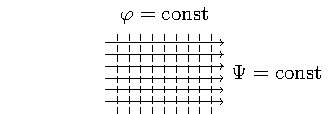
\includegraphics[scale=1.5]{img/potent}
    \caption{Однородный поступательный поток}
    \label{fig:figure1}
\end{figure}
% ---> - линии тока
% 		%B 
% % -----_*->
%  % -|--/|->
%  % -|-/-|-> v_x
%  % -|/--|-> 
% % *_----|->
% % A
% % РИС 1

% Задается вопрос на экзамене: у вас есть плоский поток, и вот такая линия по косинусу:

% \begin{figure}[h!]
%     \centering
%     \includegraphics[width=0.6\textwidth]{example-image-a}
%     \caption{Косинусоидальный профиль}
%     \label{fig:figure1}
% \end{figure}

% \begin{equation}
% 	Q=\int\limits_{A}^{B} \vec{v}\vec{n}dl=\Psi(B)-\Psi(A)=a(y_b-y_a)
% \end{equation}

% %--\
% % 	\
% % 	 \
% % 	  \
% % 	  |
% % 	  |
% % 	 /
% % 	/
% %--/
% % Линия по косинусу

\paragraph{Cопряженное течение.} $F(z)=-iF(z)=ay - i\cdot ax$:

% -|-|-|->
% -|-|-|->
% -|-|-|->
% Сопряженное течение
\begin{figure}[h!]
    \centering
    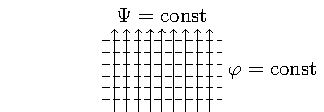
\includegraphics[scale=1.5]{img/sopr_potent}
    \caption{Сопряженное течение}
    \label{fig:figure1}
\end{figure}
$\phi=ay$, $\Psi=-ax$. Линии тока $\Psi=\const$ ортогональны линиям равного потенциала $y=\const$. Скорость $v_x=\pdv{\Psi}{y}=0$, $v_y=-\pdv{\Psi}{x}=a$.

Пусть $a=\alpha + i\beta$.
Дз. Что будут представлять из себя линии тока, если $\alpha=1,\beta=1$? Нужно найти угол наклона.

\paragraph{Cток-исток-вихрь.} В предыдущем разделе было рассмотрено поле конденсатора и поле точечного заряда. В двумерном случае рассмотрим потенциал равномерно заряженной нити.

\begin{equation}
	F(z)=m\ln(z)
\end{equation}

\begin{comment}
     |y
   ______*  
  /     /\
 /     /  \
/     / t  \
-----*--------->x
\          /
 \        /
  \______/
\end{comment}
Используем полярную систему координат
\begin{gather}
	\label{eqss}
	x=r\cos\theta\\
	y=r\sin\theta\\
	z=x+iy=re^{i\theta}\\
	F(z)=m\ln(re^{i\theta})=m\ln(r)+mi\theta
\end{gather}
\begin{comment}
Принцип действия логарифмической линейки
 ______________________________________
|_.__.__.___.___.____._____.____.______| ln x
	 ______________________________________
	|_.__.__.___.___.____._____.____.______| шкала произведения
 ______________________________________
|_.__.__.___.___.____._____.____.______| ln y

x*y
x+y

lnx+lny=ln(xy)
\end{comment}

\begin{equation}
	\phi=m\ln{r}, \quad \Psi=m\theta, \quad v_r=\pdv{\varphi}{r}=\frac{m}{r}
\end{equation}

Линии уровня $\Psi=\const$ задают радиально отходящие от центра при $m>0$ и подходящие при $m<0$ линии тока:
\begin{figure}[h!]
    \centering
    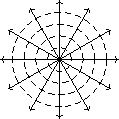
\includegraphics[scale=1.5]{img/stok-vihr}
    \caption{Линии тока при $m>0$}
    \label{fig:figure1}
\end{figure}

Посчитаем поток. 
\begin{equation}
	Q=\int\limits_{A}^{B} \vec{v}\vec{n}dl=\Psi(B)-\Psi(A)=m(\theta_b-\theta_a)
\end{equation}
Если контур является замкнутым, то $\theta_b=\theta_a$ и интеграл равен нулю.
Попробуем вычислить поток через замкнутый контур произвольного радиуса $R$, зная зависимость скорости от пространственных координат: 
\begin{equation}
	Q=\oint\limits_{A}^{B} \vec{v}\vec{ n } dl=\oint\limits_{A}^{B} v_r dl=\int\limits_{0}^{R} \frac{m}{r} \cdot 2\pi dr =2\pi m% лень писать. Говорят что надо доверять здравому смыслу
\end{equation}
Отличие величины потока, вычисленным двумя разными способами, заключается в том, что выбранный контур охватывает особую точку $r=0$. Необходимо использовать теорему о вычетах для подсчета потока первым способом. Тогда ответ совпадет со значением $Q=2\pi m$.
% \begin{figure}[h!]
%     \centering
%     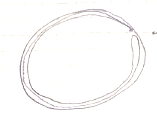
\includegraphics[width=0.6\textwidth]{photo/kontur}
%     \caption{Контур, охватывающий особую точку 0}
%     \label{fig:figure1}
% \end{figure}

\paragraph{Сопряженное течение.}
\begin{equation}
	F(z)=im\ln{z}=im\ln{re^{i \theta}}=im\ln{r}-m\theta
\end{equation}
\begin{equation}
	\phi=m\theta, \quad
	\Psi=m\ln{r}
\end{equation}
Тогда
\begin{equation}
	v_r=\pdv{\phi}{r}=0, \quad
	v_\theta=\frac{1}{r}\pdv{\phi}{\theta}=-\frac{m}{r}
\end{equation}

\begin{figure}[h!]
    \centering
    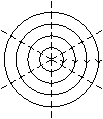
\includegraphics[scale=1.5]{img/sopr}
    \caption{Линии $\Psi=\const$}
    \label{fig:figure1}
\end{figure}
\begin{comment}
Линии Psi=const   
   ______
  /      \
 /  ._.   \
/  /   \   \
|  |   |   |
\  \._./   /
 \        /
  \______/
\end{comment}

Циркуляция:
\begin{equation}
	\Gamma=\oint \vec{v}d\vec{l}=\int \frac{m}{r}\cdot 2\pi dr=2\pi m = \const.
\end{equation}
%Течение потенциальное. Для потенциального течения циркуляция равна нулю (следствие теоремы Томсона)! Но опять, мы же захватили особую точку в середине 

Самостоятельно сделать случай $m=\alpha+i\beta$.

%$m$ мнимое -- вихрь, действительное -- сток/исток, а нужно сделать для случая $m$ комплексное.
%
%$\alpha>0$ исток (и вихрь), $\alpha<0$ сток (и вихрь). Вихрь из-за беты.
%
%Подставить и решить, как мы делали ранее:
%\begin{equation}
%	(\alpha+i\beta)\ln{re^{i\theta}}=
%		...
%\end{equation}
%
%Вообще задача качественно решается в уме. Сходящаяся или расходящаяся спираль.

Линии тока для данной задачи представляют собой спираль.
\paragraph{Гидродинамический диполь.}
\index{Диполь!гидродинамический}
\begin{equation}
	F(z)=-\frac{P}{z}=-\frac{P}{x+iy}=\phi+i\Psi
\end{equation}

\begin{figure}[h!]
    \centering
    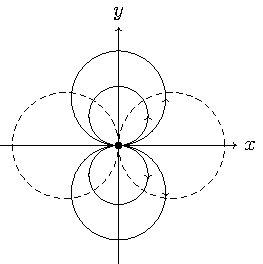
\includegraphics[scale=1.5]{img/dipol}
    \caption{Линии тока диполя}
    \label{fig:figure1}
\end{figure}
\begin{comment}
	картинка диполя:
     __>___
 \	/ _>__ \ /
  \	|/    \|/
----*      *-------
  / |\_>__/|\
 /	\__>___/ \
\end{comment}

Выражения для потенциала скорости $\phi$ и функции тока $\Psi$ примут следующий вид:
\begin{equation}
	\phi=-\frac{Px}{x^2+y^2}, \quad
	\Psi=\frac{Py}{x^2+y^2}
\end{equation}


Линии тока $x^2+y^2=c\cdot y$ -- смещенные окружности.
\begin{equation}
	x^2+y^2-2\frac{1}{2}cy+\frac{1}{4}c^2=\frac{1}{4}c^2 \quad
\end{equation}
Отсюда 
\begin{equation}
	x^2+(y-c/2)^2=\frac{1}{4}c^2=r^2,
\end{equation}
где $r=\frac{c}{2}$ -- радиус окружности, координаты центра окружности $(0,c/2)$.

Вспомним, что $\phi=-\frac{Px}{x^2+y^2}$, а $v_x=\pdv{\phi}{x}$. Тогда 
$$
v_x=\frac{P(x^2-y^2)}{(x^2+y^2)^2}
$$

% \newpage
\paragraph{Циркуляционное обтекание кругового цилиндра.} 
На круговой цилиндр радиуса $R$ слева набегает из бесконечности
(справа) поток жидкости с постоянной скоростью $v_0$.
\index{Обтекание!кругового цилиндра}
\begin{figure}[h!]
    \centering
    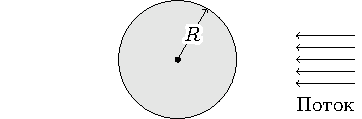
\includegraphics[scale=1.5]{img/cyl1}
    \caption{Поток, набегающий на цилиндр}
    \label{fig:figure1}
\end{figure}

На цилиндре реализовано условие непротекания, а на больших
расстояниях постоянный поток
\begin{gather}
	v_r|_{r=R}=0 \quad \text{(условие непротекания)} \\ 
	v_x|_{r\to\infty}=-v_0, \\
	v_y|_{r\to\infty}=0.
\end{gather}
В силу линейности уравнения Лапласа будем искать решение в виде
сумму двух решений, сдвиговый поток и потенциал диполя. По
отдельности они не удовлетворяют граничным условиям
\begin{equation}
	F=F_1+F_2
\end{equation}
$F_1=-v_0z$ -- набегает поток. 
$\displaystyle F_2=-\frac{A}{z}$ -- потенциал диполя

Тогда
 $$ F=-\frac{v_0}{z}-\frac{A}{z}=-v_0r e^{i\theta} -\frac{A}{r} e^{-i\theta}$$
Вычислим $v_r$:
\begin{equation}
	\pdv{\phi}{r}=-\qty(v_0-\frac{A}{r})\cos\theta
\end{equation}
Воспользовавшись граничным условиями $v_r=0$ при $r=R$, находим константу $A=v_0R^2$.

Тогда
\begin{equation}
	F=-v_0\qty(z+\frac{R^2}{z}).
\end{equation}
\begin{figure}[h!]
    \centering
	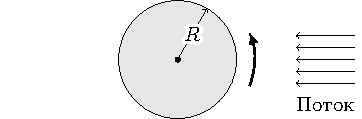
\includegraphics[scale=1.5]{img/cyl2}
    \caption{Обтекание потоком цилиндра}
    \label{fig:figure1}
\end{figure}
\begin{comment}
	   <--\
           \
   ______   \
  /	     /\  \
 /	   R/  \  \
/	   /    \  \_____
*     *     |  <----------поток набегает на 
\           /
 \         /
  \_______/
\end{comment}
Добавим течение типа «вихрь» $F_3=-\frac{\Gamma i}{2\pi}\ln{z}$.
\begin{equation}
	F=-v_0\qty(z+\frac{R^2}{z})-\frac{\Gamma i}{2\pi}\ln{z}
\end{equation}

%Что такое здесь гамма, во-первых? Посмотрим немножко назад, мы считали циркуляцию по контуру. $\Gamma=2\pi m$ Вопрос. Граничным условиям удовлетворяет? Мы конструируем решение (в силу линейности уравнения Лапласа), поэтому надо проверять. Проверяем граничные условия. Первые два слагаемых только что проверили. А добавили еще вот такое круговое течение. Добавили условие, что нормальная компонента не изменилась.
оно автоматически удовлетворяет граничным условиям. Для
потенциала и функции тока имеем
$$\phi = -v_0 \left( r+\frac{R^2}{r}\right)\cos\theta + \frac{\Gamma \theta}{2\pi}$$
Попробуйте найти самостоятельно выражение для функции тока $\Psi$.
% $$\Psi=?$$
Найдем выражение для скорости.
\begin{equation}
	v_r=\pdv{\phi}{r}=-v_0\qty(1-\frac{R^2}{r})\cos\theta
\end{equation}
\begin{equation}
	v_\theta\bigg|_{r=R}=2v_0\sin\theta+\frac{\Gamma}{2\pi R}
\end{equation}

%Смотрим на поверхность. Что на ней делается. На ней первое слагаемое: у нас обтекает поток, почему скорость в два раза больше? Понятно почему, понятно почему. А вот знак у меня правильный или неправильный? Но это не суть, важно что должен быть минус, проверьте на экзамене, ответ должен быть правильный, а не то что я написал.

%Смотрите, цилиндр:
Ниже приведены картины линий тока при разных значениях $\Gamma$.
\begin{figure}[H]
    \centering
    \noindent
	\begin{minipage}{.5\textwidth}
	\centering
	  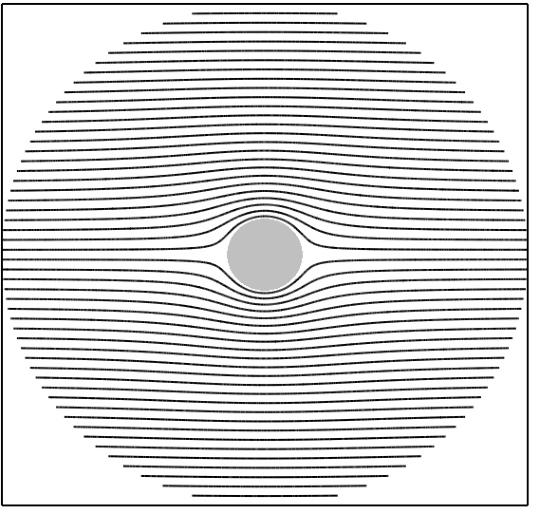
\includegraphics[width=0.7\textwidth]{photo/obtekaniecilindra1}
	\end{minipage}% This must go next to `\end{minipage}`
	\begin{minipage}{.5\textwidth}
	\centering
	  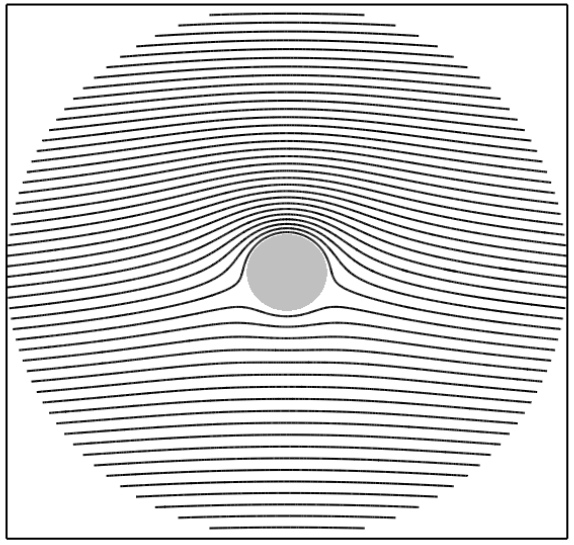
\includegraphics[width=0.7\textwidth]{photo/obtekaniecilindra2}
	\end{minipage}
    
    \caption{Линии тока при $\Gamma=0$ (слева) и $0<\Gamma<\Gamma^*$ (справа)}
    \label{fig:figure1}
\end{figure}
При добавлении кругового движения линии тока искривляются, исчезает симметрия по вертикали. При дальнейшем увеличении $\Gamma$ искривление нарастает:
\begin{figure}[H]
    \centering
    \noindent
	\begin{minipage}{.5\textwidth}
	\centering
	  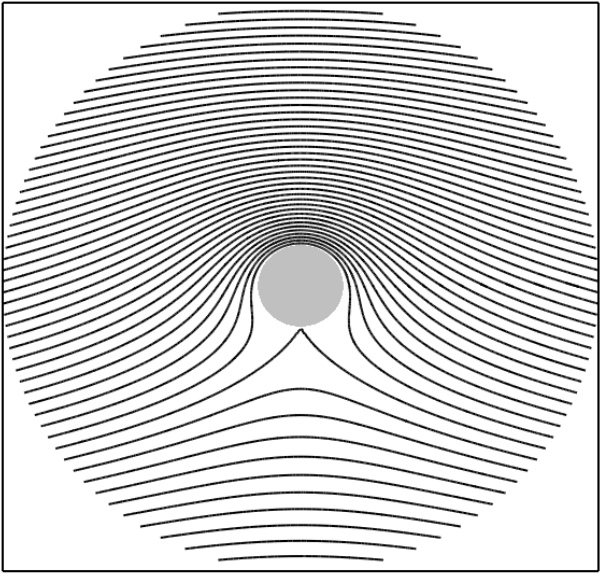
\includegraphics[width=0.7\textwidth]{photo/obtekaniecilindra3}
	\end{minipage}% This must go next to `\end{minipage}`
	\begin{minipage}{.5\textwidth}
	\centering
	  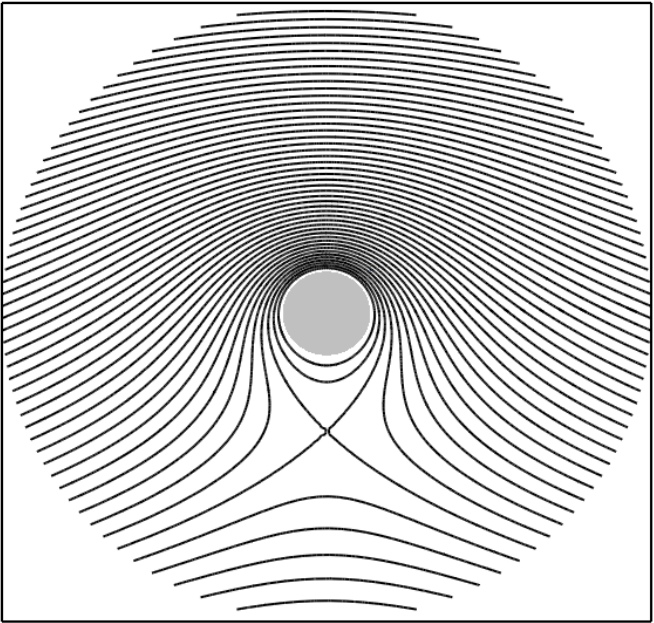
\includegraphics[width=0.7\textwidth]{photo/obtekaniecilindra4}
	\end{minipage}
    
    \caption{Линии тока при $\Gamma=\Gamma^*$ (слева) и $\Gamma>\Gamma^*$ (справа)}
    \label{fig:figure1}
\end{figure}

Критическое значение
\begin{equation}
	\Gamma^*=4\Pi v_0 R.
\end{equation}
Если гамма меньше критического, то критическая точка на поверхности цилиндра, если больше, то вне области цилиндра и появляется сепаратриса (на рисунке справа).

% \begin{figure}[H]
%     \centering
%     \includegraphics[scale=0.4]{photo/obtekaniecilindra4}
%     \caption{Сепаратриса}
%     \label{fig:figure1}
% \end{figure}
% \begin{comment}
% 	картинка с сепаратрисой. Студент Иванов построил картинки. Линии уровня.
% \end{comment}
Как видно из рисунков, при циркуляции цилиндра не нарушается
симметрия относительно миделя (то есть силы сопротивления потоку не
возникает) но над цилиндром  скорость больше чем под ним. Это обозначает возникновение подъёмной силы.

Используя уравнение Бернулли, найдем распределение давления на
поверхности цилиндра
\begin{equation}
	p_0+\frac{\rho v_0^2}{2}=p_s+\frac{\rho v_\theta^2}{2}
\end{equation}
Отсюда
\begin{equation}
	p_s=p_0+\frac{\rho}{2}\qty(v_0^2-v_\theta^2)
\end{equation}
Ну и получается
\begin{equation}
	p_s=p_0+\frac12\rho\qty(v_0^2-4v_0^2\sin^2\theta-\qty(\frac{\Gamma}{2\pi R})^2-\frac{2\Gamma v_0\sin\theta}{\pi R})
\end{equation}
Найдем силу действующую на единицу длины цилиндра со стороны
потенциального потока
\begin{equation}
	\vec{F}=-\int p\vec{n}dl.
\end{equation}

По горизонтали силы никакой нет, по вертикали вклад дает только последнее слагаемое в выражении для давления. Давление больше где скорость меньше, значит оно больше внизу, значит, возникнет подъемная сила. (скорость больше, сложение скорости набегающего потока и кругового).

\begin{equation}
	F_y=-\int p n_y \dd{l}=\rho \Gamma v_0. 
	% Место на всякий случай
\end{equation}
Это есть формула Жуковского. Сила пропорциональна плотности, скорости параметру, характеризующему вихрь.

%Для упражнения вам такой вопрос: у меня есть цилиндр, скатывающийся по наклонной плоскости. (картинка). Одна траектория в вакууме, другая в воздухе. Объяснить какая дальше.
%
%Следующий вопрос. ЧМ по футболу, угловой, мячик, мы ударяем по мячику. Объяснить как бить для сухого листа.

% лекция 22.03.2019
 
% Параграф 2.8. 
\subsubsection{Вихревые движения в идеальной жидкости}\
\index{Движение!вихревое}
До сих пор мы занимались потенциальными течениями: сток, исток, двумерное движение и так далее. Теперь рассмотрим другой класс движений идеальной жидкости -- вихревые движения.

Введем понятие вектора завихрённости $\Omega$:
\begin{equation}
	\vec\Omega=\Rot \vec{v}
\end{equation}
Завихренность можно связать с циркуляцией скорости. Для этого запишем определение циркуляции и применим теорему Остроградского-Гаусса:
\begin{equation}
	\Gamma=\oint\limits_L \vec{v} \,\dd\vec{l}
	% по теореме стокса
	=\int\limits_S \Rot \vec{v}\dd \vec{S}=\int\limits_S \vec\Omega\vec{n}\,\dd S 
\end{equation}
Это означает, что циркуляция скорости по замкнутому контуру равна потоку завихрённости.

% \begin{figure}[h!]
%     \centering
%     \includegraphics[width=0.6\textwidth]{photo/tomson}
%     \caption{}
%     \label{fig:figure1}
% \end{figure}
Воспользуемся ранее доказанной теоремой Томсона: \textit{циркуляция скорости вдоль замкнутого контура,
перемещающегося в идеальной жидкости, остается постоянной}.

Следовательно, сохраняется постоянным и поток вихря через
поверхность, натянутую на односвязный контур: $\Gamma=\const$.

Введем понятие \textit{вихревой линии} и \textit{вихревой трубки}.
Вихревой линией называют линию, касательные к которой в каждой
точке коллинеарны вектору вихря.
Если взять замкнутый контур и через каждую его точку провести
вихревую линию, то внутри образуется вихревая трубка.

% \begin{figure}[h!]
%     \centering
%     \includegraphics[width=0.6\textwidth]{example-image-a}
%     \caption{}
%     \label{fig:figure1}
% \end{figure}

% \newpage
\paragraph{Теорема Лагранжа. } \textit{Элементы идеальной жидкости, лишенные вихрей в начальный момент
	времени, будут лишены их и в дальнейшем.}


% Посмотрим теорему Лагранжа более аккуратно. 

\begin{figure}[h!]
    \centering
    \includegraphics[scale=1.5]{img/toms2}
    \caption{}
    \label{fig:figure1}
\end{figure}

На поверхности трубки разместим маленький контур $L_1$ с площадью $S_1$. Сосчитаем поток через этот маленький контур:
\begin{equation}
	\Gamma_1=\int \vec\Omega \vec{n}\dd S_1 = \oint\limits_{L_1} \vec{v} \,\dd\vec{l} = 0
\end{equation}

Так как на поверхности трубки все линии тока проходят сквозь выбранный контур в поверхности контура, то циркуляция по такому контуру будет равна нулю. 

В силу теоремы Томсона, если циркуляция $\Gamma=0$ в начальный момент времени, то она будет равна нулю и в любой дальнейший момент времени.
\qed

Вихри в идеальной жидкости возникнуть и исчезнуть не могут. Чтобы они появились, необходимы взаимодействие с поверхностью (что приводит к неодносвязности контура), и непотенциальность сил. Например, вихри могут возникнуть в заряженной жидкости в магнитном поле.
 % Маленький контур произвольный и, следовательно,лежит все времяна поверхности вихревой линии. Любое шевеление с уходом с поверхности приводит к появлению потока.
% Устремляя оба контура к нулю получаем 1 Теорему Гельмгольца.
% Вихревая линии состоит из одних и тех же элементов жидкости. Это доказательство от противного. Это была первая теорема Гельмгольца, о том, что любая линия состоит из одних и тех же элементов жидкости.

\paragraph{Вторая теорема Гельмгольца. }\textit{Поток вектора вихря через поперечное сечение лучевой трубки остается постоянным}. 

Распишем поток через поверхность лучевой трубки, представив её как объединение боковой поверхности  $S_b$ и поверхностей двух торцов $S_{1,2}$:

\begin{equation}
 	\oint \vec \Omega \vec{n} \dd S=\int\limits_{S_1} \vec \Omega \vec{n}_1 \dd S  + \int\limits_{S_2} \vec \Omega \vec{n}_2 \dd S + \int\limits_{S_b} \vec \Omega \vec{n}_b \dd S
 \end{equation} 
Очевидно, поток через боковую поверхность равен нулю. Используем формулу Остроградского-Гаусса и учитываем, что $\Div \Rot = 0$:
\begin{equation}
	\oint \vec \Omega \vec{n} dS=\iiint \Div\vec \Omega \dd V=0
\end{equation}
%Значит, поток постоянный.
Учитывая произвольность выбора поверхностей и то, что единичный
вектор нормали $\vec{n}$ меняет на торцах знак,
получаем инвариантность потока вихря через сечение вихревой трубки
\begin{equation}
	\int\limits_{S_1} \vec \Omega \vec{n} \dd S=\int\limits_{S_2} \vec \Omega \vec{n} \dd S.
\end{equation}
\textbf{Замечание}.
Если сечение достаточно мало, так что завихренность постоянна вдоль
трубки $\Omega S$, сохраняется величина $\Omega S$ -- называемая интенсивностью вихревой трубки.

Рассмотрим несколько примеров, в которых получим значение вектора завихренности.
%Если $\Omega$ можно считать константой, $S$ мало, то $\Omega S$ -- интенсивность вихревой трубки -- ?

% \begin{equation}
% 	\Div \vec{v}=0, \quad
% 	\vec \Omega=\Rot\vec{v}, \quad
% 	\pdv{\vec \Omega}{\tau}=\Rot[\vec{v},\vec{\Omega}\,]
% \end{equation}
\newpage
\paragraph{Плоское течение.} Пусть течение направлено вдоль оси $x$: $\vec{v}=(v_x(y),0,0)$.
\begin{figure}[H]
    \centering
    \includegraphics[scale=1.5]{img/vxvyvz}
    \caption{Плоское течение}
    \label{fig:figure1}
\end{figure}
Дивергенция, как нетрудно получить, равна нулю:
\begin{equation}
	\Div\vec{v}=\pdv{v_x}{x}+\pdv{v_y}{y}+\pdv{v_z}{z}=0
\end{equation}
Сосчитаем завихренность $\vec\Omega$.
\begin{equation}
	\vec{\Omega}=\mqty| % It's require package "physics"
		\vec{i}&\vec{j}&\vec{k}\\
		\pdv{x}&\pdv{y}&\pdv{z}\\
		v_x&0&0
	|=-\vec{k}\cdot\pdv{v_x}{y}
\end{equation}
Итак, завихренность есть, но она направлена либо на нас, либо от нас по рисунку. 
% Является ли данное течение стационарным? Когда у нас была гидростатика, мы находили условие равновесия, а потом проверили, будет ли это состояние стационарным. Проверка третьим уравнением, будет.
Если $v_x=b y$, то $ \vec{\Omega}=-b\vec{k}$. Это тривиальная задача.

 Рассмотрим ещё случай, когда скорость задана ступенчатой функцией. В этом случае наблюдается так называемая \textit{вихревая пелена}:
\begin{equation}
	v_x(y)=\left\{
	\begin{aligned}
		v_0&, \quad y>0\\
		0&, \quad y<0\\
	\end{aligned}
	\right.
	\quad\Rightarrow\quad
	\vec{\Omega}=\vec{k}\cdot v_0\delta(y)
\end{equation}
Найти циркуляцию можно двумя способами: сосчитать интеграл
\begin{equation}
	\Gamma=lv_0+0+0+0,
\end{equation}
или найти поток вектора завихренности
\begin{equation}
	\Gamma=\int \vec{\Omega}\vec{n}\dd S = lv_0.
\end{equation}

Мы привыкли считать, что завихренность  -- это вращение слоев жидкости. В этой задаче течение плоско-параллельное, но скорости у разных сечений разные: движение остается вихревым.

\paragraph{Вращение жидкого цилиндра.} Пусть  жидкий цилиндр радиуса $R$ вращается как твердое тело:
\begin{figure}[h!]
    \centering
    \includegraphics[scale=1.5]{img/gcyl}
    \caption{Вращение жидкого цилиндра}
    \label{fig:gcyl}
\end{figure}
% Цилиндр соосный z, 3d, ось вверх.
При этом скорость жидкости задается как
\begin{equation}
	v_\theta(r)=\left\{
	\begin{aligned}
		\omega r&, \quad r<R\\
		0&, \quad r>R\\
	\end{aligned}
	\right.
\end{equation}

Здесь можно обойтись формулой попроще. $\vec{\Omega}$ направлен по оси $z$, и получается простая формула: 
\begin{equation}
	\Rot\vec{v}=
		\vec\Omega=
		\vec{I}_z \frac{1}{r}\pdv{r}\,rv_\theta=
		2\omega\vec{I}_z, \qq{когда } r<R
\end{equation}
%(график линейный в тета от эр)
Будем считать, что снаружи от цилиндра течение потенциальное: $\vec{\Omega}=0$, тогда
\begin{equation}
 	\pdv{r} rv_\theta=0 \quad \Rightarrow \quad v_\theta=\frac{A}{r}
 \end{equation} 
Решаем
\begin{equation}
	\Gamma=\int\limits_L \vec{v}\dd\vec{l}=2\pi R\, v_\theta= 2\pi A
\end{equation}
С другой стороны, $\Gamma$ -- это поток вихря:
\begin{equation}
	\Gamma=\iint (\Rot\vec{v}, \vec{n})\dd S =\iint  \Omega_n \dd S = 2\omega\, \pi R^2
\end{equation}
Из этих формул находим
\begin{equation}
	v_\theta=\frac{\omega R^2}{r}=\frac{\Gamma}{2\pi r}
\end{equation}
Ради чего мы все это делали? Надо найти давление:
\begin{equation}
	p+\frac{\rho v^2}{2}=p_0 \quad \Rightarrow \quad
	p=p_0-\frac{\rho v^2}{2}
\end{equation}
Используем уравнение Бернулли, и ищем ошибку, которая здесь была допущена. По формуле получилось на бесконечности и в центре скорость ноль, и давление в центре нуля и на бесконечности одно и тоже. А из опыта известно, что в центре смерча, например, давление пониженное.

Подсказка: использовали уравнение Бернулли, а оно сформулировано в разных случаях: 1) для стационарного потенциального течения во всем пространстве, 2) вдоль лучевой трубки, 3) нестационарное

При $r>R$ можно пользоваться, течение потенциальное. А внутри-то там есть вихрь, течение не потенциально, и формулой Бернулли пользоваться нельзя.

% Непонятно как получается такая формула:
\begin{equation}
	r>R: p=p_0-\frac{\rho\omega^2 R^4}{2r^2}
\end{equation}

Внутри пользуемся уравнением Эйлера. Как мы его выводили: масса умножить на ускорение равно силе.
\begin{equation}
	\pdv{v}{t}+\vec{v}\,\nabla\vec{v}=-\frac{\nabla p}{\rho}
\end{equation}
У нас $\pdv{v}{t}=0$. Нужно знать $\vec{v}\,\nabla\vec{v}$ в сферической системе координат. Есть два способа: первый - посмотреть, второй - смотрим на картиночку: частичка движется по окружности, радиус у неё известен $R$, скорость известна $\omega r$. Ускорение центростремительное $a_r=-\frac{v^2}{R}=-\omega^2 r$. Тогда можем записать:
\begin{equation}
	-\omega^2 r  = - \dv{p}{r}\frac{1}{\rho}
\end{equation}
\begin{equation}
	p(r)=\left\{
	\begin{aligned}
		&p_0-\frac{\rho\omega^2 R^4}{2r^2}&, \quad& r>R\\
		&p_0-\frac{\rho\omega^2 R^4}{R^2}+\frac{\rho\omega^2 r^2}{2}&, \quad& r<R\\
	\end{aligned}
	\right.
\end{equation}
\begin{figure}[H]
    \centering
    \includegraphics[scale=1.5]{img/pr}
    \caption{Зависимость давления от расстояния}
    \label{fig:figure1}
\end{figure}
Получается, что давление в центре меньше, чем на бесконечности. Чем больше радиус вихря, тем меньше давление.


%Если кто-то хочет подумать. Вихрь имеет такую \/ структуру. Попробуйте показать, что в нем есть подъемная сила.


%Займемся следующим приближением.
\subsubsection{Точечные вихри}
\index{Вихри!точечные}

Устремляем сечение нашей вихревой трубки к нулю так:
\begin{equation}
	R\to0, \quad \omega\to\infty, \quad 
	\Gamma=2\pi \omega R^2 =2\pi A, 
	\quad v_\theta=\frac{\Gamma}{2\pi r}
\end{equation}

Пусть у нас есть много вихрей: 
\begin{figure}[H]
    \centering
    \includegraphics[scale=1.5]{img/vihri}
    \caption{Много вихрей}
    \label{fig:vihri}
\end{figure}
Как они между собой будут взаимодействовать? У нас есть уравнение Лапласа, которое работает всюду, кроме вихревых линий. Скорость в данной точке равняется суперпозиции скорости от всех вихрей. Дальше, по теореме Гельмгольца, завихренность переносится частицами жидкости. То есть, скорость точечного вихря $\Gamma_i$ равняется скорости жидкости в данной точке, создаваемой всеми остальными вихрями. 

\begin{equation}
	\dv{\vec{r}_i}{t}=\sum\limits_{k\ne i} \vec{v}_k (\vec{r}_i)
\end{equation}

% (чисто техническая картиночка)
\begin{figure}[H]
    \centering
    \includegraphics[scale=1.5]{img/vihr_coord}
    \caption{Координаты вихря}
    \label{fig:figure1}
\end{figure}
\begin{comment}	
	y
	^
	|
y_i	|- - - - * Г_i
	|   .  ` '
	|._______'_______> x
	         x_i
\end{comment}
\begin{equation}
	r=\sqrt{ (x_k-x_i)^2+(y_k-y_i)^2 }, \quad
	\sin\theta=\frac{y_i-y_k}{r}, \quad v_\theta=\frac{\Gamma_k}{2\pi r_{ik}}
\end{equation}
Первое:
\begin{equation}
	\dv{x_i}{t}=-\frac{1}{2\pi}\sum\limits_{k\ne i} \frac{\Gamma_k (y_i-y_k)}{r^2_{ik}}
\end{equation}
\begin{equation}
	\dv{y_i}{t}=-\frac{1}{2\pi}\sum\limits_{k\ne i} \frac{\Gamma_k (x_i-x_k)}{r^2_{ik}}
\end{equation}
Какие интегралы есть у этой системы?
\begin{equation}
	\sum \Gamma_i\dv{x_i}{t}=-\sum\sum \frac{\Gamma_k\Gamma_i (y_i-y_k)}{r^2_{ik}}=0
\end{equation}
Это значит, что
\begin{equation}
	\sum x_i \Gamma_i=\const=\overline{x}\sum \Gamma_i, \qq{где} \overline{x}=\frac{\sum x_i \Gamma_i}{\sum \Gamma_i}
\end{equation}
Тривиально, что то же самое можно записать по координате $y$. Если $n>2$, других интегралов нету.

% Если есть желающие, попробуйте составить программу, которая бы решала эту систему уравнений. Мышкой ставить точку, какая интенсивность гаммы i вводится, мышкой вторая точка ставится интенсивность, и т.д. каждая точка своим цветом, старт, картинки крутятся и вертятся.

% Если есть два вихря противоположных знаков, то они уходят на бесконечность: нужно динамическое изменение области просмотра.


Рассмотрим более простую задачу. Всего два вихря: $r_1$ и $r_2$.
\begin{equation}
	\dv{x_1}{t}=-\frac{\Gamma_2 (y_1-y_2)}{2\pi r^2}, \quad r^2=\sqrt{(x_1-x_2)^2+(y_1-y_2)^2}.
\end{equation}
\begin{equation}
	\dv{x_2}{t}=\frac{\Gamma_1 (y_1-y_2)}{2\pi r^2}, \quad r^2=\sqrt{(x_1-x_2)^2+(y_1-y_2)^2}.
\end{equation}
\begin{equation}
	\dv{y_1}{t}=\frac{\Gamma_2 (x_1-x_2)}{2\pi r^2}, \quad r^2=\sqrt{(x_1-x_2)^2+(y_1-y_2)^2}.
\end{equation}
\begin{equation}
	\dv{y_2}{t}=-\frac{\Gamma_1 (x_1-x_2)}{2\pi r^2}, \quad r^2=\sqrt{(x_1-x_2)^2+(y_1-y_2)^2}.
\end{equation}
Домножаем, складываем:
\begin{equation}
	\Gamma_1 x_1 + \Gamma_2 x_2=\const, \quad
	\Gamma_1 y_1 + \Gamma_2 y_2=\const
\end{equation}
Мы нашли два интеграла: центр тяжести не изменяется.
Ну, давайте попробуем еще найти интегралы. Если мы найдем еще два интеграла, то задачу сделаем. Подсказка: из первого уравнения вычесть второе.
\begin{gather}
	\dv{t}\qty(x_1-x_2)=-\frac{\qty(\Gamma_1+ \Gamma_2)}{2\pi}\frac{y_1-y_2}{r},\\
	\dv{t}\qty(y_1-y_2)=\frac{\qty(\Gamma_1+ \Gamma_2)}{2\pi}\frac{x_1-x_2}{r}
\end{gather}
Домножаем, складываем:
\begin{gather}
	(x_1-x_2)\dv{x_1-x_2}{t}+(y_1-y_2)\dv{y_1-y_2}{t}=0 \quad \Rightarrow \quad \\ \Rightarrow\quad
	\dv{(x_1-x_2)^2}{t}+\dv{(y_1-y_2)^2}{t}=0
\end{gather}
Отсюда еще один интеграл
\begin{equation}
	(x_1-x_2)^2+(y_1-y_2)^2=r^2=\const	
\end{equation}

Вихри вращаются вокруг неподвижного центра тяжести, с сохранением расстояния между ними. Какие при этом траектории движения? Чтобы найти траекторию, из первого уравнения находим $x_1$, из второго $y_2$, подставляем в это уравнение и получим уравнение окружности.

а) Что же у нас теперь будет? Посмотрим частный случай, когда $\Gamma_2=0$, $\Gamma_1=\Gamma$. (рис) Движение по окружости $v_\theta=\frac{\Gamma}{2\pi r}$, центр тяжести в точке ненулевого вихря.

\begin{figure}[H]
    \centering
    \includegraphics[scale=1.75]{img/oneG}
    \caption{}
    \label{fig:oneG}
\end{figure}

б) Два вихря $\Gamma, \Gamma$ -- центр тяжести посередине, расстояние между вихрями $l$, $v_\theta=\frac{\Gamma}{2\pi l}$.

\begin{figure}[H]
    \centering
    \includegraphics[scale=1.75]{img/twoG}
    \caption{}
    \label{fig:twoG}
\end{figure}

в) Два вихря $\Gamma, -\Gamma$. Центр тяжести будет находится на бесконечности (нетрудно посчитать). $v=\frac{\Gamma}{2\pi l}$. Два таких вихря двигаются с постоянной скоростью.

\begin{figure}[H]
    \centering
    \includegraphics[scale=1.75]{img/3G}
    \caption{}
    \label{fig:3G}
\end{figure}

г) Вихрь над плоскостью. Метод изображений даст, что вихри будут двигаться параллельно плоскости.

\begin{figure}[H]
    \centering
    \includegraphics[scale=1.75]{img/4g1}
    \caption{}
    \label{fig:figure1}
\end{figure}

д) Вихрь в угле будет двигаться на бесконечности параллельно линиям угла. Для нахождения траектории можно использовать метод изображений:

\begin{figure}[H]
    \centering
    \includegraphics[scale=1.75]{img/5G}
    \caption{}
    \label{fig:figure1}
\end{figure}

e) Цепочка вихрей после обтекания цилиндра -- цепочка Кармана.
\begin{figure}[H]
	\centering
	\includegraphics[width=0.6\textwidth]{example-image-a}
	\caption{Цепочка Кармана}
	\label{fig:figure5}
\end{figure}
% Вставить рис 6 Карман
% (если получится)


% % Лекция 29.03.
% На прошлой лекции для совокупности вихрей:
% \begin{gather}
% 	\label{eqga}
% 	\dv{\vec{\Gamma_i}}{t}=\sum v_k(\Gamma_i), \quad v_k=\frac{\Gamma_k}{2\pi r_{ik}}
% \end{gather}

\newpage
\subsection{Поверхностные гравитационные волны}
\index{Волны!поверхностные!гравитационные}

Надо отметить большое разнообразие волновых движений в
жидкостях и газах. Это волны на поверхности жидкости, внутренние
волны в океане. 

Мы будем рассматривать гравитационные волны на поверхности
несжимаемой жидкости. Если ровная поверхность жидкости выведена
из состояния равновесия, то под действием силы тяжести возмущение
стремится вернутся в равновесие и возникнет колебательное движение.


К таким волнам относятся корабельные волны, цунами, ветровые волны, внутренние волны в неоднородной жидкости. При исследовании мы будем использовать ряд приближений. Во-первых, жидкость должна быть \textbf{идеальная и несжимаемая} (нет вязкости, звука). Также она должна быть \textbf{однородна} (плотность постоянна). При этом \textbf{поверхность жидкости плоская и неограниченная} (земля в данных масштабах плоская). Кроме того, мы будем рассматривать только волны \textbf{малой амплитуды}.

\begin{figure}[H]
    \centering
    \includegraphics[scale=1.5]{img/simple_wave}
    \caption{Характеристики волны}
    \label{fig:simplewave}
\end{figure}

\begin{comment}

       |<------ l ----->|
   ________        ___________
  /        \       /          ^
/           \ _ _ /           | a
------------------------------------------
\end{comment}
Оценим слагаемые в уравнении Эйлера:
\begin{gather}
	\label{eq}
	\pdv{\vec{v}}{t}+(\vec{v},\nabla)\vec{v}=-\frac{\nabla p}{\rho}+\vec{g}
\end{gather}
\begin{gather}
	\label{eq}
	\pdv{v}{t}\sim\frac{v}{\tau}, \quad 
	A\sim V\tau, \quad \tau \sim \frac{A}{v},
	\quad \pdv{v}{t}\sim \frac{v^2}{a}, 
	\quad (\vec{v},\nabla)\vec{v}\sim \frac{v^2}{l},
	\quad l\gg a
\end{gather}
Значит, вторым слагаемым можно пренебречь, и тогда
\begin{gather}
	\label{eq}
	\pdv{\vec{v}}{t}=-\frac{\nabla p}{\rho}-\nabla(gz)
\end{gather}
Берем от этого уравнения ротор:
\begin{equation}
	\Rot\Grad=0, \quad
	\Rot\vec{v}=0, \quad \vec{v}=\Grad\phi,
\end{equation}
Из несжимаемости
\begin{equation}
	\Div\vec{v}=0
\end{equation}
Тогда
\begin{equation}
	\nabla^2\phi=0.
\end{equation}
Волны описываются (в отсутствии силы тяжести и постоянной плотности воды) уравнением Лапласа. 
% Давайте подумаем, откуда же что делается. 
% Давайте напишем граничные условия.
% \begin{figure}[H]
%     \centering
%     \includegraphics[width=0.6\textwidth]{example-image-a}
%     \caption{}
%     \label{fig:figure1}
% \end{figure}

\begin{figure}[H]
    \centering
    \includegraphics[scale=1.5]{img/simple_wave2}
    \caption{Новые координаты}
    \label{fig:simplewave2}
\end{figure}

\paragraph{Решение задачи о волнах.} Введем новую координату $\xi=z-z_0$  для решения задачи так, как это показано на рисунке \ref{fig:simplewave2}. Начнем решение задачи с поверхности волны: это граница с воздухом, значит, есть некое давление $p_0$. Можем вернуться к уравнению Эйлера, вместо скорости подставить $\nabla\phi$, и тогда мы получим нестационарное уравнение Бернулли
\begin{equation}
	\Grad\qty(\pdv{\phi}{t}+\frac{p}{\rho_0}+gz)=0,
\end{equation}
откуда следует, что на поверхности жидкости
\begin{equation}
	\rho\pdv{\phi}{t}+\rho g\xi=-p_0,
\end{equation}
где введено малое смещение волны от плоскости $\xi(x,y,t)$.

Переопределим потенциал, чтобы избавиться от $p_0$, добавлением не зависящей от координат величины $p_0t/\rho$. Тогда условие на поверхности примет вид
% Первое приближение: всегда можем ввести $\phi'=p_0\rho t+\phi$
% Второе приближение: возмущения достаточно малы, и получится
\begin{equation}
	\rho\pdv{\phi}{t}\bigg|_{z=\xi}+\rho g\xi=0 \quad 
\end{equation}
Найдем, чему равняется вертикальная скорость:
\begin{equation}
	v_z=\dv{\xi}{t}=\pdv{\xi}{t}+\xcancel{(v_z\Grad)\xi},
\end{equation}
здесь из-за малости колебаний вторым слагаемым мы пренебрегли,  и тогда
\begin{equation}
	v_z=\dv{\xi}{t}=\pdv{\xi}{t}
\end{equation}
С другой стороны, 
\begin{equation}
	v_z=\pdv{\xi}{t}=\pdv{\phi}{z}
\end{equation}
Продифференцировав по времени уравнение для $\phi$ и заменив $\pdv{\xi}{t}$ на $\pdv{\phi}{z}$, получим окончательно граничное условие  на потенциал:
\begin{equation}
	\pdv[2]{\phi}{t}\bigg|_{z=0}+g\pdv{\phi}{z}\bigg|_{z=0}=0
\end{equation}
В силу малости возмущений мы заменили граничное условие на поверхности жидкости на граничное условие на плоскости $z=0$. Граничное условие на поверхности мы получили выше. Еще нужно граничное условие на дне -- условие непротекания: вертикальная компонента скорости на дне равна нулю:
\begin{equation}
	\pdv{\phi}{z}=0 \bigg|_{z=-H}
\end{equation}
Если волны идут в однородном полупространстве, то в качестве второго
граничного условия берем $\phi \to 0$ при $z\to\infty$.

Введем волновую замену потенциала $\phi=\Phi(z)\cdot e^{i(kx- \omega t)}$. Тогда уравнение Лапласа примет вид
\begin{equation}
	\dv[2]{\Phi}{z}-k^2\Phi=0
\end{equation}
Оно взялось из $\nabla^2\phi=0$. Нам надо найти такое решение, чтобы оно удовлетворяло нулю на дне. 

Будем искать решение в виде
\begin{equation}
	\Phi=A\ch{k(z+H)},
\end{equation}
тогда
\begin{equation}
	\phi=A\ch{k(z+H)}\cdot e^{i(kx- \omega t)}.
\end{equation}
Считаем производные:
\begin{equation}
	\pdv{\phi}{z}=Ak\sh{k(z+H)}\cdot e^{i(kx- \omega t)}
\end{equation}
\begin{equation}
	\pdv[2]{\phi}{t}=-\omega^2A\ch{k(z+H)}\cdot e^{i(kx- \omega t)}
\end{equation}
В итоге получаем дисперсионное уравнение:
\begin{gather}
	\label{eq:disp}
	-\omega^2A\ch{k(z+H)}\cdot e^{i(kx- \omega t)}+gAk\sh{k(z+H)}\cdot e^{i(kx- \omega t)}=0 \bigg|_{z=0}
	\\ \Rightarrow \quad
	\omega^2=gk\th{kH} = gk \frac{e^kH-e^{-kH}}{e^{kH}+e^{-kH}} = gk\frac{\sh kH}{\ch x}
\end{gather}


% \begin{figure}[H]
%     \centering
%     \includegraphics[scale=1]{photo/tanh.jpg}
%     \caption{График $\th{x}$}
%     \label{fig:figure1}
% \end{figure}

% У нас есть два масштаба: длина волны $\lambda$ и глубина водоема $H$.



\paragraph{Траектории частиц в волне. } Нас интересует, как двигаются частицы. Запишем потенциал:
\begin{equation}
	\phi=A\ch{k(z+H)}\cdot\exp(ikx-i\omega t)
\end{equation}
% Частичка находится на некотором горизонте. У нас 
% \begin{equation}
% 	v_x=\pdv{\phi}{x}, \quad v_z=\pdv{\phi}{z}
% \end{equation}
% (потом посчитаем)
% Дальше у нас есть координаты: 
% \begin{equation}
% 	\dv{\xi}{t}=v_x, \quad \dv{\eta}{t}=v_z
% \end{equation}
% В результате мы сможем определить траектории, по которым двигается частица.
% % Лекция 05.04.2019
% % -------------------
% На дне мы задействовали условие непротекания, наверху нестационарное уравнение Бернулли. 
% В результате мы решили уравнение, использовав граничные условия, и получили дисперсионное соотношение.
% \begin{equation}
%     \phi = A \ch{k(z+H)}\exp(i(kx-\omega t)), \quad
%     v = \nabla \phi
% \end{equation}
% Мы находимся на некотором горизонте $z$:
Найдем компоненты скоростей на высоте $z$:
\begin{equation}
    v_x = \pdv{\phi}{x} = ikA\ch{k(z+H)}e^{i(kx-\omega t)}
\end{equation}
\begin{equation}
    v_z = \pdv{\phi}{z} = kA\sh{k(z+H)}e^{i(kx-\omega t)} 
\end{equation}
Отсюда
\begin{gather}
    \dv{\xi}{t} = v_x, \quad \xi=\frac{v_x}{-i\omega} = -\frac{kA}{\omega}\ch{k(z+H) e^{i(kx-\omega t)} }\\
    \dv{\eta}{t} = v_z, \quad \eta=\frac{v_z}{-i\omega} = \frac{ikA}{\omega}\sh{k(z+H) e^{i(kx-\omega t)} } \\
\end{gather}
При $z = 0$ у нас $\xi = a$ (амплитуда на поверхности равна амплитуде колебаний):
\begin{equation}
    a = \xi|_{z = 0} = \frac{ikA}{\omega}\sh{kH}
\end{equation}
Поскольку величины у нас комплексные, мы должны взять действительную часть. После нехитрых математических операций смещения частицы по вертикали ($\xi$) и по горизонтали ($\eta$) найдутся в виде
\begin{gather}
    \xi = -\frac{a}{\sh{kH}}\ch{k(z+H)}\sin{(kx-\omega t)}\\
    \eta = \frac{a}{\sh{kH}}\sh{k(z+H)}\cos{(kx-\omega t)}\\
\end{gather}
Отсюда видно, что траектории двигаются по эллипсу:
\begin{equation}
    \frac{\xi^2}{a_\xi^2}+\frac{\eta^2}{a_\eta^2} = 1, 
    \quad a_\xi = \frac{a\ch{k(z+H)}}{\sh{kH}}
    , \quad a_\eta = \frac{a\sh{k(z+H)}}{\sh{kH}}
\end{equation}
% Надо рассмотреть два случая.


\subsubsection{Волны на мелкой воде}
\index{Волны!поверхностные!на мелкой воде}
Как следует из названия этого раздела, мы будем рассматривать волны на мелкой воде, где будем работать в приближении $\lambda \gg H$ или, что тоже самое,  $kH\ll 1$.

Дисперсионное уравнение \eqref{eq:disp} для волн на мелкой воде примет вид
\begin{equation}
	\omega^2=gk^2H, \quad \omega=\pm k\sqrt{gH}
\end{equation}
Зависимость от $k$ линейная, значит, \textit{волны на мелкой воде -- это волны без дисперсии}. Яркий пример волн без дисперсии -- это цунами в океане. Глубина океана 5-6 км, а цунами имеет длину волны десятки -- сотни километров.


% $v_\text{f}=v_\text{gr}$, если у нас волны на мелкой воде и $v_\text{f}=v_\text{gr}=\sqrt{gH}$.

У нас есть понятие фазовой и групповой скоростей:
\begin{equation}
	v_\text{f}=\frac{\omega}{k}, \quad
	v_\text{gr}=\dv{\omega}{k}
\end{equation}

Если воспользоваться соответствующим дисперсионным уравнением, окажется, что для волн на мелкой воде фазовая и групповая скорости совпадут.

Если у нас есть некий волновой пакет, и мы смотрим как он распространяется, у нас есть огибающая и есть фаза. Групповая скорость - скорость огибающей, фазовая - скорость постоянной фазы:
\begin{figure}[H]
    \centering
    \includegraphics[scale=1.5]{photo/wavelet.pdf}
    \caption{Распространение волнового пакета}
    \label{fig:wavelet}
\end{figure}

% Нарисуем графики, как выглядит фазовая скорость для волн на мелкой воде:

% \begin{figure}[H]
%     \centering
%     \includegraphics[scale=1.2]{photo/vf.jpg}
%     \caption{График фазовой скорости}
%     \label{fig:vph}
% \end{figure}



Теперь уточним вид траекторий частицы в мелкой волне. Ранее мы нашли, то что в любом случае это движение по эллипсу с амплитудами $a_\xi, a_\eta$. Найдем их в случае $kH\ll 1$, для этого разложим гиперболические функции  в ряд Тейлора при малых аргументах:
\begin{equation}
    \sh{x}\approx x+\ldots, \quad \ch{x}\approx 1+\ldots
\end{equation}
Учтем ещё, что в выбранной нами системе координат (ось $z$ вверх, на глубине $z$ отрицательны) $k(z+H)<kH$. Тогда из полученных ранее формул несложно получить
\begin{equation}
    a_\xi = \frac{a}{kH}, \quad
    a_\eta = a\qty{1+\frac{z}{H}}
\end{equation}
Частички двигаются по сильно вытянутым эллипсам.

% (картинка с эллипсом и волной)
\begin{figure}[H]
    \centering
    \includegraphics[scale=1.5]{img/ellipse2}
    \caption{Движение частиц на разной глубине}
    \label{fig:ellipse2}
\end{figure}



\subsubsection{Волны на глубокой воде}
\index{Волны!поверхностные!на глубокой воде}

В этом случае $kH \gg 1$. Тогда $\tg kH$ равен 1, и тогда дисперсионное уравнение примет вид
\begin{equation}
	\omega=\pm\sqrt{gk}
\end{equation}
Волна не чувствует дно, но появляется сильная дисперсия. 

Найдем фазовую и групповую скорости:
\begin{equation}
	v_\text{f}=\sqrt{\frac{g}{k}}, \qquad v_\text{gr}=\frac{g}{2\sqrt{gk}}=\frac12 v_\text{f}
\end{equation}


На мелкой воде пакет волн двигается вместе, а на глубокой гребни волн будут убегать вперед\footnote{
 Задание к экзамену: оценить время расплывания пакета (рис. \ref{fig:wavelet}) из второй производной
$$
	\pdv[2]{\omega}{k} 	
$$ }


Определим траектории частиц. По определению, 
\begin{equation}
    \sh{x} = \frac{e^x+e^{-x}}{2}, \quad \ch{x} = \frac{e^x-e^{-x}}{2}
\end{equation}
Отбросив некоторые слагаемые по порядку малости, получим
\begin{equation}
    \sh{kH}\approx\ch{kH}\approx \frac{e^{kH}}{2} 
\end{equation}
После подстановки в формулы для эллипсов получим
\begin{equation}
    a_\xi = a_\eta = ae^{kz}, \quad z<0
\end{equation}
Траектории представляют собой окружности, радиус которых быстро спадает с глубиной. 

Займёмся численным экспериментом. 
Оценка такая: мы находимся в море, амплитуда волны $a$ равна 5 метрам.
Это очень серьёзные волны. 
Давайте считать, что длина волны $\lambda=10$  метров, а мы опустились на глубину 10 метров.
Какая будет амплитуда колебаний частиц? Если посчитать, то будет один сантиметр. Вот так быстро спадает. Наверху шторм, а на глубине фактически стоит штиль.

\begin{figure}[H]
    \centering
    \includegraphics[width=0.6\textwidth]{example-image-a}
    \caption{}
    \label{fig:figure1}
\end{figure}


% \paragraph{Резюме.} Длинные волны -- это волны без дисперсии, траектории продолговатые эллипсы. $v_\text{f} = v_\text{gr} = \sqrt{gH}$. 
% \begin{equation}
%     \pdv{\xi}{t}+v\pdv{\xi}{x} = 0 ???, \xi = \xi_0(x-vt)
% \end{equation}
% Выйдем за пределы и будем считать, что
% \begin{equation}
%     v = \sqrt{g(H+\xi)}
% \end{equation}
% Попробуйте представить себе, что будет. Волна подходит к берегу, и возникает два эффекта: за счёт малой $H$, энергия то никуда не девается, амплитуда становится больше. Второй эффект в возрастании скорости гребня (быстрее чем подошва), и волны опрокидывается. 

% Короткие волны -- это волны с дисперсией, и их траектории -- окружности. При этом $v_\text{f} = \frac{\omega}{k} = \ldots$, $v_\text{gr} = \dv{\omega}{k}$

\newpage
\subsection{Гравитационно-капиллярные волны}
\index{Волны!поверхностные!гравитационно-капиллярные}
Ранее мы не учитывали поверхностное напряжение. Нарисуем картинку

% (картинка)
\begin{figure}[H]
    \centering
    \includegraphics[scale=1.5]{img/2rad}
    \caption{Два главных радиуса кривизны}
    \label{fig:2rad}
\end{figure}

Есть два главных радиуса кривизны, и возникает избыточное давление:
\begin{equation}
    \delta p_s = \alpha\qty(\frac{1}{R_1}+\frac{1}{R_2}) = \alpha \frac{1}{R} = -\alpha\nabla \qty(\frac{\nabla\xi}{\sqrt{1+(\nabla\xi)^2}})
\end{equation}
Если $\nabla\xi \sim \frac{a}{\lambda} \ll 1$, то $\delta p_s = -\alpha \Delta \xi$.

Задача свелась к предыдущей. Граничное условие на дне -- непротекание, а на поверхности за счет сил поверхностного натяжения граничное условие изменится:
\begin{equation}
    \rho\pdv{\phi}{t}+\rho g\xi+p_0+\delta p_s = 0, \quad z = 0
\end{equation}
% (градиент выкинули в силу линейности задачи, считаем колебания малыми)

От $p_0$ мы избавляемся аналогично предыдущей задаче, и в итоге получаем граничное условие:
\begin{equation}
    \pdv{\phi}{t}+g\xi+\alpha\Delta\xi = 0 \quad\bigg|_{z = 0}
\end{equation}
% Что дальше с этим делать? То же самое, что и раньше. У нас встретились $\phi$ и $\xi$, надо от $\xi$ избавиться. Вспоминаем:
% \begin{equation}
    % \Delta\xi = \pdv[2]{\phi}{x}
% \end{equation}
% ??? 
 Продифференцируем уравнение по времени и вспомним что 
\begin{equation}
	v(z) = \pdv{\xi}{t}=\pdv{\phi}{z}
\end{equation}
% 𝑣𝑧 =
% 𝜕𝜉/𝜕𝑡=𝜕𝜙/𝜕𝑧
В результате получаем граничное условие:
\begin{equation}
    \pdv[2]{\phi}{t}+g\pdv{\phi}{z}-\frac{\alpha}{\rho}\frac{\partial^3\phi}{\partial z^2 \partial t} = 0
\end{equation}
Как и раньше, внутри слоя воды мы имеем для потенциала уравнение Лапласа.
Решаем уравнение Лапласа, учитываем граничные условия на дне, и получаем  решение для потенциала
\begin{equation}
	\phi=𝐴\ch k(z + 𝐻).
\end{equation}
Теперь подставляем это решение в последнее уравнение, и получаем дисперсионное уравнение:
\begin{equation}
    \omega^2 = (gk+\gamma k^3)\th{kH}, \quad \gamma = \frac{\alpha}{\rho}.
\end{equation}
\begin{equation}
    kH \gg 1 \quad \Rightarrow \quad \omega^2 = gk+\gamma k^3.
\end{equation}
Когда же волны существенно капиллярны? Для ряби на воде, например. Понятно, что для цунами этот эффект незначителен. Давайте найдём фазовую скорость:
\begin{equation}
    v_\text{f}^2 = \frac{\omega^2}{k^2} = \frac{g}{k}+\gamma k 
\end{equation}
Такая зависимость имеет минимум, как показано на графике:
\begin{figure}[H]
    \centering
    \includegraphics[scale=1.5]{img/min}
    \caption{График с минимумом, $\lambda_0 = 1.7 \text{ см}$}
    \label{fig:figure1}
\end{figure}
% (график с минимумом) 

Ищем, чему равен минимум: он равен $k_{*} = \sqrt{\frac{g}{k}}$

\begin{equation}
    v_\text{gr} = \dv{\omega}{k} \quad \Rightarrow \quad 
    v_\text{gr} = \frac{v_\text{f}}{2}\frac{k_{*}^2+3k^2}{k_{*}^2+k^2}
\end{equation}

При очень маленьких $k$ $v_\text{gr} = \frac{v_\text{f}}{2}$ (как на мелкой воде). 
При больших же $v_\text{gr} = \frac{3}{2}v_\text{f}$.
Итак, у нас есть капиллярные и гравитационные волны.
В одном случае групповая скорость меньше фазовой, в другой больше фазовой. 

\paragraph{Резюме: гравитационные и гравитационно-капиллярные волны.}
Дисперсионное уравнение:
\begin{equation}
    \omega^2 = (gk+\gamma k^3)\th{kH}
\end{equation}
Если $k \gg k_*$, это капиллярные волны. 
Если $\frac{1}{H} \ll k \ll k_*$, то это гравитационные короткие волны (дно ещё не чувствуется).
Если же $k \ll \frac{1}{H}$, то это длинные гравитационные волны.


\paragraph{Задача о устойчивости.} Попробуем обсудить случай, когда у нас есть слои жидкости, причем тяжелая жидкость сверху. 
Здесь мы возвращаемся к гидростатике.
Является ли такое состояние решением уравнения гидростатики? (вверху тяжелея, внизу лёгкая).
Гравитация параллельна градиенту плотности, это хорошо. 
А является ли такое состояние устойчивым? 

Нужно написать уравнение Лапласа, поставить граничные условия, написать дисперсионное уравнение с учётом капиллярных сил. 
Считаем, что поверхность достаточно недалеко.

%надо переставить одну спичку
Задача отличается от предыдущей лишь тем, что мы фактически перевернули её вверх ногами. Тогда можно получить правильное  уравнение дисперсии просто сменой знака $g$:
\begin{equation}
    \omega = \sqrt{-gk+\gamma k^3}
\end{equation}

% \begin{figure}[H]
%     \centering
%     \includegraphics[width=0.6\textwidth]{example-image-a}
%     \caption{}
%     \label{fig:figure1}
% \end{figure}

Тут возникают проблемы: отрицательные $\omega^2$ при $k < k_* = \sqrt{\frac{g}{k}}$. Если $k>k^*$ (мелкие возмущения), то всё нормально:
\begin{equation}
    \omega_{1,2} = \pm\sqrt{\gamma k^3}
    \quad \Rightarrow \quad
    \xi = c_1e^{i\omega_1 t}+c_2e^{i\omega_2 t}
\end{equation}
А при мнимых $\omega$:
\begin{equation}
    \xi = c_1e^{-|\omega|t}+c_2e^{|\omega|t}
\end{equation}

Итак, при малых возмущениях жидкость просто колеблется,а при больших начинает течь.

Значит, решение устойчивое. Простой пример из жизни -- это перевернутый флакон духов. Бутылочку можно перевернуть вверх ногами, но духи не вытекут:
потому что горлышко узкое, и масштабы маленькие, а $k$ большое (подавлены крупномасштабные возмущения). 

Из жизненного опыта известно, что в таком случае духи надо потрясти: действительно, согласно Эйнштейну, движение с ускорением эквивалентно увеличению силы тяжести:
\begin{equation}
    k_{*\text{э}} = \sqrt{\frac{g+a}{k}}
\end{equation}

% Следующий раздел -- внутренние волны/
\newpage
\subsection{Внутренние волны}
\index{Волны!внутренние}

% Задать малые возмущения, лианеризовать и т.д. Частота Брента-Вейсаля.

% На следующей лекции рассмотрим простую задачу двухслойной жидкости $\rho_1, \rho_2$.
% Ось зет вверх, зададим возмущение на поверхности и надо решить эту задачу.

% Решение ищем в виде бегущей волны, считаем что вверх и вниз убывает (экспоненциально).
% Граничные условия: на границе одинаковая скорость ($\dv{\phi_1}{z} = \dv{\phi_2}{z}$).
% Ещё одно граничное условие -- давление на поверхности: сверху и снизу границы давление одинаково.

% В итоге напишем дисперсионное уравнение. В пределом случае получим гравитационные волны (при $\rho_1 \to 0$).

% 12.04
Пусть у нас есть устойчивая стратификация жидкости: жидкость двухслойная, с плотностями слоев $\rho_2>\rho_1$.
% Итак, у нас такая задача:
\begin{figure}[H]
    \centering
    \includegraphics[scale=1.5]{img/vnutr}
    \caption{Внутренние гравитационные волны}
    \label{fig:vnutr}
\end{figure}
Считаем, что до границы достаточно далеко.
На границе есть какие-то возмущения
% (рисунок)
\begin{equation}
    \Delta\phi_1 = 0, \quad \Delta\phi_2 = 0
\end{equation}
Справа налево начнём писать уравнение.
Будем искать решение в виде
\begin{gather}
    \phi_1 = A e^{-kz} e^{i(kx-\omega t)}\\
    \phi_2 = B e^{kz} e^{i(kx-\omega t)}\hphantom{^{-}}
\end{gather}
% \begin{equation}
%     \phi_1 = \Phi(z)\cdot e^{i(kx-\omega t)}
% \end{equation}

Наша задача -- найти дисперсионное уравнение. Займёмся константами. Мы по-прежнему считаем, что колебания относительно малы,
т.е. амплитуда колебаний много меньше длины волны.

Из кинематического граничного условия, нормальная компонента скорости на границе раздела слоев непрерывна:
\begin{equation}
    v_z = (\approx) \pdv{\xi}{t} = \pdv{\phi_1}{z} = \pdv{\phi_2}{z}
\end{equation}
Отсюда сразу следует $B = -A$.

Мы должны поставить второе граничное условие. Используем нестационарное уравнение Бернулли:
\begin{equation}
    p_1 = -\rho_1 g \xi - \rho_1 \pdv{\phi_1}{t}, \qquad
    p_2 = -\rho_2 g \xi - \rho_2 \pdv{\phi_2}{t}
\end{equation}
Здесь мы пренебрегли слагаемым $v^2$ в силу малости колебаний.
Граничные условия -- давления на поверхности одинаковы:
\begin{equation}
    kg(\rho_2-\rho_1) = \omega^2(\rho_2+\rho_1)
\end{equation}
Мы избавились от $\xi$ и в итоге получаем дисперсионное уравнение:
\begin{equation}
    \omega = \sqrt{gk\frac{\rho_2-\rho_1}{\rho_2+\rho_1}} \approxeq \sqrt{gk\frac{\Delta \rho}{\rho}}
\end{equation}
Предельный случай: $\rho_1 \to 0$ даёт переход к случаю гравитационных волн на глубокой воде. 
В океане $ \frac{\Delta\rho}{\rho}\sim 10^{-2}$.

\paragraph{Мертвая вода.} В 1893 г. знаменитый норвежский полярник Фритьоф Нансен, совершавший плавание по арктическим водам, столкнулся со странным явлением. Вот что записал он в отчете: \textit{<<Мы почти не двигались с места \dots и будто тащили всю воду за собой. Что мы ни делали, -- круто поворачивали, лавировали, описывали полный круг и пр., -- все напрасно. Лишь только машина переставала работать, судно тотчас же останавливалось, точно схваченное чем-то за корму».}
\index{Мертвая вода}

Встречается явление лишь там, где слой пресной или
сильно распресненной воды лежит поверх соленой морской воды.
Впрочем, чтобы «попасться», как попалось судно Нансена, нужно еще одно
совпадение: толщина верхнего пресного слоя должна примерно
равняться толщине судна. Тогда на малом ходу его винт будет
расходовать почти всю свою энергию не на движение вперед,
а на создание внутренних волн на границе двух слоев воды -- корабль
почти замирает на месте, при этом сами волны с корабля незаметны.

Переход к частоте Брента-Вяйсяля:
\begin{equation}
    \pdv{\vec{v}}{t}+(\vec{v}\,\nabla)\vec{v} = -\frac{\nabla p}{\rho}+\vec{g}
\end{equation}
\begin{equation}
	\pdv{\rho}{t}+\Div \rho \vec{v} = 0
\end{equation}

Уравнение гидростатики:
\begin{equation}
    \dv{p_0}{z} = -g \rho_0(z)
\end{equation}

\begin{equation}
    \pdv{\vec{v}}{t} = -\frac{\nabla p_0+\nabla p_1}{\rho_0+\rho'}+\vec{g}
\end{equation}

Несжимаемость даст
\begin{equation}
    \dv{\rho}{t} = 0 \quad \Rightarrow \quad
    \Div \vec{v} = 0
\end{equation}

Нетривиальность в следующем: не хватает одного уравнения: переменных 5, уравнений скалярных 4.

Вспомним полную производную:
\begin{equation}
    \pdv{\rho}{t}+\Div \rho \vec{v} = 0
\end{equation}
\begin{equation}
    \pdv{\rho}{t}+(\vec{v}\,\nabla)\rho = 0
\end{equation}
Это записано для возмущений. $\rho = \rho_0+\rho'$:
\begin{equation}
    \pdv{\rho'}{t}+(\vec{v}\,\nabla)[\rho_0+\rho'] = 0
\end{equation}
% \begin{equation}
    % (\vec{v}\,\nabla(\rho_0+\rho'))
% \end{equation}
Пренебрежём $\vec{v}\,\nabla \rho'$, тогда получим ещё уравнение
\begin{equation}
    \pdv{\rho'}{t}+v_z\dv{\rho_0}{z} = 0
\end{equation}

Вспомним и запишем частоту Брента-Вяйсаля:
\begin{equation}
    N^2 = -g\dv{\rho_0}{z}\frac{1}{\rho_0}
\end{equation}
Тогда последнее уравнение перепишем в виде
\begin{equation}
    \pdv{\rho'}{t}-v_z \frac{N^2}{g}p_0 = 0
\end{equation}
Таким образом у нас появилась частота Брента-Вяйсяля, которая ранее возникала при качественном рассмотрении рассмотрении вопроса об устойчивости стратифицированной жидкости. Обычно еще делается предположение о малости стратификации. Это так называемое \textit{приближение Буссинеска}.  Мы не будем приводить эти выкладки.
% Это уравнение  в \textit{приближении Буссинеска}.

Без всякого вывода рассмотрим один частный случай: экспоненциальная атмосфера, где $\rho_0(z) = \rho_0 e^{-\frac{z}{H}}$, и $N^2 = gH$. 
\begin{equation}
    v_z = A\exp{-i\omega t+ik_xx+ik_zz}
\end{equation}
Здесь $H$ -- эффективная высота атмосферы. Дисперсионное уравнение здесь будет
\begin{equation}
    \omega^2 = N^2\cdot k_x^2
\end{equation}
Можно записать так:
\begin{equation}
    \omega = N\sin\theta, \qq{где} \sin{\theta} = \frac{k_x}{k}
\end{equation}
1) Волны существуют только с частотой $\omega<N$.
2) Зависимость направления от частоты. Если $\omega \to N$, то волновой вектор направлен горизонтально. Если же $\omega \ll N$, напротив, вертикально.
3) $\vec{v_\text{f}} \perp \vec{v}_{gr}$:
\begin{figure}[H]
    \centering
    \includegraphics[scale=1.5]{img/vol}
    \caption{}
    \label{fig:vol}
\end{figure}
% 
% Рисунок с профилем звука в волноводном канале. 
% Из закона сохранения нужно найти закон спадания.
% \begin{equation}
   % p^2\cdot 2\pi r l \quad \Rightarrow \quad p \sim \frac{1}{r} 
% \end{equation}

% Попробуем решить такую задачу. В районе Англии произошла катастрофа: взорвались торпеды у подводной лодки. Во сколько раз будет больше акустическое давление в волноводном канале по сравнению с сферической волны? $H \sim 100$ м, мы на побережье Америки. $\sqrt{\frac{l = 5000}{H = 0.1}} \approx 7000$.

\newpage
\section{Движение вязкой несжимаемой жидкости}

Мы уже столкнулись с рядом парадоксов: парадокс Даламбера -- на тело в потоке идеальной жидкости не действует сила. Из жизненного опыта хорошо известно, что это не так. Второй недостаток теории идеальной жидкости -- невозможность образования вихрей. 

Наконец, для идеальной жидкости у нас было граничное условие непротекания: отсутствовала нормальная компонента скорости. Но это вступает в противоречие с опытным фактом: на поверхности неподвижного тела равен нулю модуль скорости. Это происходит из-за наличия сил молекулярного сцепления между жидкостью и твердым телом. Следствием этого является следующий <<парадокс>>: на лопастях крутящегося вентилятора собирается пыль. 

\subsection{Уравнения гидродинамики вязкой жидкости}

Займёмся получением уравнений, которые учитывали бы вязкость и разрешали вышеперечисленные парадоксы. Для этого мы можем использовать закон сохранения массы (уравнение неразрывности), так как мы его получили без дополнительного предположения об отсутствии вязкости:
\begin{equation}
    \pdv{\rho}{t}+\Div \rho \vec{v} = 0
\end{equation}
Для идеальной жидкости мы смогли получить уравнение Эйлера:
\begin{equation}
    \pdv{\vec{v}}{t}+(\vec{v}\,\nabla)\vec{v} = -\frac{\nabla p}{\rho}+\vec{g}
\end{equation}
Для вязкой жидкости его вывести уже не получится. Мы будем конструировать уравнение с помощью экспериментальной задачи.

\paragraph{Экспериментальная задача.} Пусть у нас есть две пластины. Нижняя бесконечная пластина (плоскость) неподвижна, а верхняя пластина площади $S$ находится на высоте $h$ над нижней. К верхней пластине мы прикладываем силу $F$, и она двигается с постоянной скоростью $v$.

Из опытов известно: чтобы пластинка двигалась с постоянной скоростью, нужно выполнение равенства
\begin{equation}
	\label{eq:fsev}
    \frac{F}{S} = \eta \frac{V_0}{h}
\end{equation}
здесь $\eta$ -- это \textit{динамический коэффициент вязкости}. Для жидкости он убывает с ростом температуры, а для газов медленно растёт.
Принято также вводить вязкость на единицу массы -- так называемую \textit{кинематическую вязкость}.
\begin{equation}
    \nu = \frac{\eta}{\rho}.
\end{equation}

\begin{table}[H]
\centering
\begin{tabular}{lll}
\toprule
Вещество при $20^\circ$ & $\eta$, $\frac{\text{г}\cdot\text{см}}{\text{с}}$ & $\nu$, $\frac{\text{см}^2}{\text{с}}$ \\ \midrule
 вода &	0.010 &	0.010 \\
воздух & $1.8\cdot10^{-4}$ & 0.15 \\
спирт &	0.018 &	0.022 \\
глицерин &	8.5 &	6.8 \\
ртуть &	0.0156 &	0.0012 \\\bottomrule
\end{tabular}
\end{table}

Из таблицы видно, что для движения воздуха вязкость оказывается более существенной, чем для воды. 


% Будем постепенно переходить к уравнениям. Мысленно выберем в жидкости небольшую площадочку: $\Delta x, \Delta y, \Delta z$.

% \begin{figure}[H]
%     \centering
%     \includegraphics[width=0.6\textwidth]{example-image-a}
%     \caption{}
%     \label{fig:figure1}
% \end{figure}

% По аналогии можем записать:
% \begin{equation}
%     \frac{\Delta F}{\Delta S} = \eta \frac{\Delta v_x}{\Delta x}
% \end{equation}
\paragraph{Конструирование уравнений Навье-Стокса.} Попытаемся сконструировать (но не вывести!) уравнения движения вязкой жидкости.
За основу возьмём закон сохранения импульса. Он фундаментален и верен и для вязкой жидкости, в отличие, например, от закона сохранения энергии, который уже использовать нельзя: вязкость есть внутреннее трение, значит есть диссипация.
\begin{equation}
	\label{eq:zsi}
    \pdv{t}\rho v_i = -\pdv{\Pi_{ik}}{x_k}, \qq{где}
    \Pi_{ik} = p \delta_{ik}+\rho v_i v_k+\sigma_{ik}
\end{equation}

Добавили одно слагаемое -- тензор вязких напряжений $\sigma_{ik}$. 
Попробуем его собрать на основе логичных предположений.

Во-первых, очевидно -- если жидкость двигается или вращается как целое, то внутреннего трения нет. Трение возникает только при относительном смещении слоёв жидкости (значит, в тензор войдут производные скоростей по координатам, то есть градиенты скорости).

Второе -- мы не рассматриваем экстремальные движения, и считаем что зависимость ($\sim \eta$) линейна. Вязкие силы возникают на молекулярных масштабах и все величины в гидродинамике медленно меняются на этих масштабах.

Наконец, жидкость будем считать изотропной. В таких предположениях можно записать наиболее общий вид тензора вязких напряжений (это тензор 2-го ранга):
{\color{red}
\begin{equation}
	\label{eq:sigmaik}
    \sigma_{ik} = a\qty(
        \pdv{v_i}{x_k}+\pdv{v_k}{x_i}
    )+
    c\qty(
       \pdv{v_i}{x_k}-\pdv{v_k}{x_i}
    )+
    b\sum \pdv{v_i}{x_k} \delta_{ik}
\end{equation}
Рассмотрим случай вращения жидкости как целого:
\begin{equation}
	\label{eq:vomegar}
    \vec{v} = [\vec{\Omega}\times \vec{r}\,]  =
    \mqty|
    \vec{i} & \vec{j} & \vec{k}\\
    \Omega_x & \Omega_y & \Omega_z\\
    x& y & z
    | \quad \Rightarrow \quad
    \begin{aligned}
    	v_x = \Omega_y z - \Omega_z y,\\
    	v_y = \Omega_x z - \Omega_z x, \\
    	v_z = \Omega_x y - \Omega_y x
    \end{aligned}
\end{equation}
Прямая подстановка \eqref{eq:vomegar} в \eqref{eq:sigmaik} даёт
\begin{equation}
    \pdv{v_i}{x_k}+\pdv{v_k}{x_i} = 0, \quad
    \sum \pdv{v_i}{x_k} \delta_{ik} = 0
\end{equation}
Так как при вращении жидкости как 	целого тензор вязких напряжений равен нулю, а мы получили равенство нулю двух из трех слагаемых тензора, то очевидно, третье тоже равно нулю.
Так как в общем случае
\begin{equation}
    \pdv{v_i}{x_k}-\pdv{v_k}{x_i} \ne 0,
\end{equation}
единственным вариантом остается положить в \eqref{eq:sigmaik} константу $c=0$.

Посмотрим внимательнее на последнее слагаемое в \eqref{eq:sigmaik}. Оказывается, это не что иное, как дивергенция:
\begin{equation}
    \sum \pdv{v_i}{x_k} \delta_{ik} = 
    \pdv{v_1}{x_1}+\pdv{v_2}{x_2}+\pdv{v_3}{x_3} = \Div \vec{v}
\end{equation}
это слагаемое существенно, только если жидкость сжимаема.
 % Резюме:
% \begin{equation}
%     \sigma_{ik}= \eta\qty(
%         \pdv{v_i}{x_k}+\pdv{v_k}{x_i}
%     )+ \xi\sum \pdv{v_i}{x_k} \delta_{ik}
% \end{equation}

% Программа следующей лекции: у нас есть уравнение, выражение для тензора $\Pi_{ik}$, и т.п. Должны получить уравнения Навье-Стокса -- cистема дифференциальных уравнений в частных производных движения вязкой ньютоновской жидкости.

%Лекция от 19.04.2019
% Мы взяли за основу уравнение (потому что есть закон сохранения импульса, который выполняется и для вязкой среды):
% \begin{equation}
%     \pdv{t}\rho v_i = -\pdv{\Pi_{ik}}{x_k}-\sigma_{ik}, \quad 
%     \Pi_{ik} = p\delta_{ik} + \rho v_i v_k
% \end{equation}
% Импульс меняется за счёт сил. Первое слагаемое -- за счёт давления, второе -- за счет (прослушал).
% Ещё добавили тензор вязких напряжений $\sigma$. В результате, предполагая что жидкость изотропна
% и матрица из 9 элементов симметрична, получаем три константы. После предположения о вращении
% жидкости как целого, избавились ещё от одной константы и получили
Переобозначим константы $a=\eta$, $b=\xi$. Тогда тензор вязких напряжений перепишется как
\begin{equation}
    \sigma_{ik} = \eta \qty(\pdv{v_i}{x_k}+\pdv{v_k}{x_i})+\xi \sum\limits_l \pdv{v_l}{x_l} \delta_{ik}
\end{equation}
Воспользуемся уравнением непрерывности $\pdv{\rho}{t} = -\pdv{x_k} \rho v_k$, подставив его в закон сохранения импульса \eqref{eq:zsi}:
\begin{gather}
    % \pdv{t} \rho v_i = 
     % -\pdv{x_k}\qty( {p \delta_{ik}}+{\rho v_i v_k}+\sigma_{ik} )\\
     \pdv{t} \rho v_i = \pdv{\rho}{t}v_i + \rho \pdv{v_i}{t} =  -v_i \pdv{x_k} \rho v_k + \rho \pdv{v_i}{t} =  -\pdv{\Pi_{ik}}{x_k}\\
     -v_i \pdv{x_k} \rho v_k + \rho \pdv{v_i}{t} =
     	-\pdv{x_k}\qty( \vphantom{\frac{1}{2}} {p \delta_{ik}}+{\rho v_i v_k}+\sigma_{ik} )
\end{gather}
Раскроем правую часть уравнения:
\begin{gather}
	-\pdv{\Pi_{ik}}{x_k}=
	-\pdv{x_k}\qty(\vphantom{\frac{1}{2}} {p \delta_{ik}}+{\rho v_i v_k}+\sigma_{ik} )=\\=
	-\pdv{p_k}{x_k}-v_i\pdv{x_k}\rho v_k-v_k\pdv{x_k}\rho v_i-\pdv{\sigma_{ik}}{x_k}
\end{gather}
Продифференцируем отдельно тензор вязких напряжений:
\begin{equation}
	-\pdv{\sigma_{ik}}{x_k}=-\eta\pdv[2]{v_i}{x_k}-\eta\pdv{v_k}{x_i}{x_k}-
	\ldots
\end{equation}
}
% Надо суметь продифференцировать эти (?) слагаемые. Это элементарная работа, далее вместо производной плотности 
% задействуем уравнение непрерывности.
% \begin{equation}
%     \pdv{x_k} \rho v_i v_k = v_i \pdv{x_k} \rho v_k + v_k \rho \pdv{v_i}{x_k}
% \end{equation}
% Замечание:
% \begin{equation}
%     \pdv{p\delta_{ik}}{x_k} = \pdv{p_k}{x_k}
% \end{equation}
После подстановки тензора, дифференцирования и перегруппировки слагаемых получим
\index{Уравнение!Навье-Стокса}
\begin{equation}
    \rho\qty(
        \pdv{v_i}{t}+v_k\pdv{v_i}{x_k}
    )=
    -\pdv{p}{x_i}+\eta\pdv[2]{v_i}{x_k}+\qty(\frac{\eta}{3}+\xi)\pdv[2]{v_k}{x_i x_k}
\end{equation}
Это и есть уравнение Навье Стокса\footnotemark. Его можно также записать в векторной форме:
\footnotetext{Уравнения Навье-Стокса -- система дифференциальных уравнений в частных производных, описывающая движение вязкой ньютоновской жидкости. Уравнения Навье-Стокса являются одними из важнейших в гидродинамике и применяются в математическом моделировании многих природных явлений и технических задач. Названы по имени французского физика Анри Навье и британского математика Джорджа Стокса.
В анализе решений уравнений заключается суть одной из семи <<проблем тысячелетия>>, за решение которых Математический институт Клэя назначил премию в 1 млн. долларов США. Необходимо доказать или опровергнуть существование глобального гладкого решения задачи Коши для трёхмерных уравнений Навье-Стокса. Нахождение общего аналитического решения для пространственного или плоского потока осложняется тем, что оно нелинейное и сильно зависит от начальных и граничных условий.
}
\begin{equation}
    \rho\qty(\pdv{\vec{v}}{t}+(\vec{v}\,\nabla)\vec{v}\,) = -\nabla p + \eta \Delta \vec{v} +
   \qty(\frac{\eta}{3}+\xi)\Grad\Div \vec{v}
\end{equation}
Часто также употребляется форма записи через кинематическую вязкость $\nu=\eta/\rho$:
\begin{equation}
    \pdv{\vec{v}}{t}+(\vec{v}\,\nabla)\vec{v} = -\frac{\nabla p}{\rho}+\nu \Delta \vec{v}
\end{equation}
Размерность кинематического коэффициента вязкости, как нетрудно видеть из уравнения Навье-Стокса,
\begin{equation}
    [\nu] = \frac{L^2}{T}
\end{equation}

\paragraph{Диссипация в несжимаемой вязкой жидкости.} Для несжимаемой вязкой жидкости $\Div \vec{v}=0$, а значит, тензор вязких напряжений упростится:
\begin{equation}
	 \sigma_{ik} = \eta\qty(\pdv{v_i}{x_k}+\pdv{v_k}{x_i})
\end{equation}
При этом диссипация энергии, по определению
\begin{equation}
	E_k = \frac{\rho}{2}\int v^2 \dd{V}
\end{equation}
Из этих формул и уравнения Навье-Стокса можно показать (доказательство можно посмотреть в \href{http://www.immsp.kiev.ua/postgraduate/Biblioteka_trudy/GidrodinamikaLanday1986.pdf#page=76}{Ландау, т.6 <<Гидродинамика>>, стр. 76}), что 
\begin{equation}
    \pdv{E_k}{t} = \frac{\rho}{2} \int 2\pdv{v_i}{t} v_i \dd{V}=
    -\frac{\eta}{2} \int   \qty(\pdv{v_i}{x_k}+\pdv{v_k}{x_i})^2 \dd{V}
\end{equation}

\paragraph{Определение коэффициентов в уравнении Навье-Стокса.} Как определять коэффициенты $\eta$, $\xi$, которые мы ввели при конструировании тензора вязких напряжений? Мы конструировали уравнения, не выводя их строго, и поэтому потеряли возможность получить аналитические выражения для коэффициентов, и их надо как-то определять экспериментально.

Можно взять круглый диск (касающийся жидкости) на нити, закрутить и определить добротность осциллятора с затуханием. Можно бросить шарик в сосуд. Или прокачивать жидкость через трубу, и скорость вытекания будет как-то зависеть от вязкости.

Рассмотрим такую задачу:

\begin{figure}[h!]
    \centering
    \includegraphics[scale=1]{img/voda}
    \caption{}
    \label{fig:figure1}
\end{figure}

Верхняя поверхность жёсткая... Рассмотрим стационарный случай:
\begin{equation}
    \pdv{t} = 0
\end{equation}
Кроме того,
\begin{equation}
    \pdv{\Pi_{ik}}{x_k} = 0,\quad
    \Pi_{ik} = p\delta_{ik}+\rho v_i v_k -\sigma_{ik}
\end{equation}
Проинтегрируем это уравнение по внутреннему объёму:
\begin{equation}
    \int\limits_S \Pi_{ik} \eta_k \dd{S} + \int\limits_{S'} \Pi_{ik} \eta_k \dd{S} = 0
\end{equation}
На внутренней поверхности, если жидкость идеальная, то равна нулю нормальная компонента: для вязкой же жидкости равен нулю модуль скорости. Тогда
\begin{equation}
    F_i = -\int p \eta_i \dd{S} - \underbrace{\int \nabla_{ik} \eta_k \dd{S}}_{F'_i}
\end{equation}
У нас есть две силы: первая -- обычное давление, и вязкая сила на единицу поверхности:
\begin{equation}
    f'_i = \sigma_{ik} n_k
\end{equation}
Дурацкий вопрос: скорость равна нулю, а откуда возникает сила? А из равенства нулю скорости не следует равенство нулю градиента.

Будем использовать достаточно часто.

В принципе, мы можем найти силу, с которой жидкость действует на тело, измеряя силу $F'$.

Если каким-то способом удалось измерить скорости и градиенты вдали от тела, то можно по ним найти, чему равна сила.

% Должно быть очевидно, что
% \begin{equation}
%     F_i = F'_i
% \end{equation}
% (не успел написать почему)
\paragraph{Замечание о граничных условиях.} У твердого неподвижного тела скорость на поверхности равна нулю.

\begin{figure}[h!]
    \centering
    \includegraphics[scale=1.5]{img/tv}
    \caption{}
    \label{fig:figure1}
\end{figure}
\begin{equation}
    \vec{v}= (v_x (y),0,0)
\end{equation}
Наверху жидкости никакой нет, поэтому
\begin{equation}
    f_i = \sigma_{ik} n_k =
    \eta\pdv{v_x}{y} = 0
\end{equation}

\newpage
\subsection{Течение Куэтта}
\index{Течение!Куэтта}
Плоское течение между двумя пластинками 
\begin{figure}[h!]
    \centering
    \includegraphics[scale=1.5]{img/kuett}
    \caption{}
    \label{fig:figure1}
\end{figure}

Запишем уравнение Навье-Стокса:
\begin{equation}
    \rho\qty(
        \pdv{v_i}{t}+v_k\pdv{v_i}{x_k}
    )=
    -\pdv{p}{x_i}+\eta\pdv[2]{v_i}{x_k}+f_i
\end{equation}
Начнём упрощать:
\begin{equation}
    \pdv{t} = 0,\quad
    \vec{v} = \qty(v_x (y),0,0), \quad
    p = p(y)
\end{equation}
В этих предположениях 
\begin{equation}
    -\pdv{p}{y} = -g, \quad
    p = p_0 + \rho_0 g y
\end{equation}
Запишем уравнение в проекции на ось ..
\begin{equation}
    \eta\pdv[2]{v_x}{y} = \pdv{p}{y} = 0
\end{equation}
И здесь граничные условия
\begin{equation}
    v_x (0) = 0, \quad
    v_y (H) = V_0
\end{equation}
Будем искать решение в виде $v_x (y) = cy$, тогда
\begin{equation}
    cH = V_0 \quad \Rightarrow \quad c= \frac{V_0}{H}
\end{equation}

В конечном итоге, важно знать силу, действующую на площадку. Мы хотели найти именно её.
\begin{equation}
    f_i = \sigma_{ik} n_k 
\end{equation}
В нашем случае $n_k \equiv n_y = -1$, в таком случае
\begin{equation}
    f_y = -\eta \pdv{v_x}{y}= -\eta \frac{V_0}{H}
\end{equation}
Умножив её на площадь, получим первую экспериментальную формулу, которую мы получили \ref{eq:fsev}. Вывод был нестрогим, и мы сразу ввели константу $\eta$. Более строго следовало ввести произвольную константу и определить из эксперимента, что она совпадает с $\eta$.

\subsection{Течение Пуазейля}
\index{Течение!Пуазейля}
\begin{figure}[h!]
    \centering
    \includegraphics[scale=1.5]{img/puaz}
    \caption{Постановка задачи}
    \label{fig:figure1}
\end{figure}
Будем рассматривать стационарное течение $v = v(r)$  с граничным условием $v(R)=0$ -- на поверхности трубы у нас скорость равняется нулю. 

Запишем уравнение Навье-Стокса в векторной форме:
\begin{equation}
    \pdv{\vec{v}}{t}+(\vec{v}\,\nabla)\vec{v} = 
    - \frac{\nabla p}{\rho}+\nu \Delta \vec{v}
\end{equation}
В левой части стоит ускорение. У нас частички все двигаются по прямой с постоянной скоростью, значит, скорость и градиент будут сонаправлены и скалярное произведение $(\vec{v}\,\nabla)=0$. Значит, вся левая часть обращается в нуль. 

Считаем, что внешних сил никаких нет, тогда получаем уравнение (при этом подставим $\nu = \frac{\eta}{\rho}$):
\begin{equation}
    \pdv{p}{z} = \eta 
   \qty[
   \frac{1}{r} \pdv{r} r \pdv{v}{r}
   ]
\end{equation}
Отсюда первое тривиальное заключение
\begin{equation}
    \pdv{p}{z} = c_1
\end{equation}
Тогда
\begin{gather}
    \eta\frac{1}{r} \pdv{r} r \pdv{v}{r} = с_1
    \quad \Rightarrow \quad
    \eta r\pdv{v}{r} = c_1 \frac{r^2}{2} + c_{1}\\
    v = \qty(\dv{p}{z}) \frac{r^2}{4\eta}+A \ln(r) + B
\end{gather}
Из физической реализуемости (скорость в центре трубы должна ) $A = 0$, а из условия
\begin{equation}
    v(R) = 0 \quad \Rightarrow \quad
    v(r) = \qty(\dv{p}{z}) \frac{1}{4\eta}\qty(r^2-R^2)
\end{equation}

Если вода бежит вправо, то слева давление больше, и градиент скорости отрицательный. Тогда профиль скорости будет таким:

\begin{figure}[h!]
    \centering
    \includegraphics[scale=1.5]{img/puaz_prof}
    \caption{Профиль скорости в задаче Пуазейля}
    \label{fig:figure1}
\end{figure}

Сосчитаем поток:
\begin{equation}
    Q=2\pi \int\limits_0^R v(r) r \dd{r} =
    \frac{\pi}{8\eta} \qty(\pdv{p}{z})\cdot R^4
\end{equation}
Там, где самая большая скорость (в центре), элемент площади при интегрировании очень мал. Поэтому получается такая зависимость.

Что будет, если в трубу вложить еще одну трубу таким образом, чтобы поток бежал между трубами по цилиндрическому слою? Тогда исчезает нерегулярность логарифма, и константа $A$ не исчезает. Придётся ставить два граничных условия, на обеих трубах.

Интересно сделать предельных переход от такой задачи о вложенных трубах к случаю, когда радиус внутренней трубы  стремится к нулю. Это нужно проделать очень аккуратно.

Последний комментарий по этой задаче -- найдём силу:
\begin{equation}
    f_z = \eta_{ik} n_k = -\sigma_{zr} = -\eta \pdv{v_r}{r}=
    -\frac{1}{2} \qty(\dv{p}{z})R
\end{equation}

\newpage
\subsection{Нестационарное движение вязкой жидкости. Вязкие волны}
\index{Волны!вязкие}

Постановка задачи такая: у нас гармонически колеблется пластинка, над пластинкой размещена жидкость. Как она будет колебаться?
\begin{figure}[h!]
    \centering
    \includegraphics[scale=1.5]{img/koleb}
    \caption{Задача}
    \label{fig:figure1}
\end{figure}
Запишем уравнение Навье-Стокса для несжимаемой жидкости (из соображений симметрии $\vec{v}=(v_x (z),0,0)$, очевидно):
\begin{gather}
    \Div \vec{v} = 0 \quad \Rightarrow \quad \pdv{v_z}{z} = 0\\
    \pdv{v_x}{t} = \nu \pdv[2]{v_x}{z}
\end{gather}
Будем искать решение уравнения диффузии в виде 
\begin{equation}
    v_x = A e^{i\omega t + ikz}
\end{equation}
Тогда
\begin{equation}
    -i \omega = \nu k^2 \quad \Rightarrow \quad
    k = \pm(1+i) \sqrt{\frac{\omega}{2\nu}}
\end{equation}
Можно ввести величину \textit{скин-слоя}:
\begin{equation}
    \delta=\sqrt{\frac{2\nu}{\omega}}
\end{equation}
При этом корни дисперсионного уравнения будут записываться как
% left 26.04.2019
% Мы занимаемся нестационарными движениями вязкой жидкости.
% Ища решение в виде (), мы получили дисперсионное уравнение (). 
% При этом можно ввести понятие скин-слоя (). С ним
\begin{equation}
    k=\pm (1+i) \frac{1}{\delta}
\end{equation}
Тогда решение будет в виде
\begin{equation}
    v_x=(Ae^{ik_1 z}+Be^{ik_2 z})e^{i\omega t}
\end{equation}
Считая, что на бесконечности ничего нет, получим
\begin{equation}
    v_x=v_0 e^{-\frac{z}{\delta}} \exp[-i \frac{z}{d}+ i\omega t]
\end{equation}
Поскольку среда вязкая, возмущения передаются наверх, но затухают на характерном масштабе толщины скин-слоя. Второй сомножитель описывает запаздывание. 

Можно подумать о поведении профиля скорости при разных положениях пластинки. Например, пластинка в крайнем правом положении -- профиль скорости приведен на рис. \ref{fig:krai}. Подумайте над случаем, когда скорость пластинки максимальна (посередине колебательного цикла).

\begin{figure}[tb]
    \centering
    \includegraphics[scale=1.5]{img/krai}
    \caption{Профиль скорости при крайнем положении пластинки (когда пластинка неподвижна)}
    \label{fig:krai}
\end{figure}

\paragraph{Комментарий об уравнении теплопроводности.} Это уравнение ности разные названия: параболическое, диффузионное, теплопроводности. 

Есть известная задача: на поверхности земли мы выкопали погреб. По мере опускания вниз годовые вариации температуры запаздывают примерно на полгода: зимой доходит летнее тепло, и наоборот. 

% \begin{equation}
%     I=\int \phi(t) e^{i\omega t} \dd{t}=
%     \int \phi(t) e^{2\pi f t} \dd{t}=
%     -\int \phi(t) (e^{i_2\pi})^{ft} \dd{t}=
%     \int \phi(t) 1^{ft} \dd{t} \ne \int \phi(t) \dd{t}
% \end{equation}

% Где $\phi(t)$ -- плавная функция, а $e^{i\omega t}$ -- быстрые осцилляции. Надо обвести в рамочку это отступление.

Вернемся к задаче. Чтобы двигать пластину, нужно приложить силу:
\begin{equation}
    f=ma, \quad a=v_0 \omega
\end{equation}
Качественно представим себе, как зависит сила от толщины слоя жидкости $H$. Нужно поставить граничное условие на поверхности: свободная граница -- $\pdv{v_x}{z}=0$.

\begin{figure}[tb]
    \centering
    \includegraphics[scale=1.5]{img/fH}
    \caption{f(H)}
    \label{fig:figure1}
\end{figure}

Если мы наливаем очень тонкий слой, то жидкость движется целиком (из жизненного опыта). Если толщина меньше скин-слоя $\delta$, то движение происходит без запаздывания, и $f \sim H$. Если наливать еще больше воды, то будет двигаться слой порядка $\delta$. Тогда сила выйдет на константу.

Также можно представить себе аналогичную задачу, когда верхняя граница не свободна, а неподвижна. По-прежнему, когда $H \gg \delta$, сила будет константой. Гораздо интереснее, когда слой становится тоньше.

Также подумайте, как будет выглядеть зависимость силы от частоты $f(\omega)$.

% \begin{figure}[tb]
%     \centering
%     \includegraphics[]{example-image-a}
%     \caption{}
%     \label{fig:figure1}
% \end{figure}

\index{Принцип!подобия}
\subsection{Принцип подобия. Формула Стокса}
Когда мы рассматривали идеальную жидкость, мы рассматривали достаточно сложные движения, по сложным траекториям, там были ускорения и т.д.
\begin{equation}
	\label{eq:eil}
    \pdv{\vec{v}}{t}+(\vec{v},\nabla\,)\vec{v}+\frac{\nabla p}{\rho}=
    \nu \Delta \vec{v} + g \vec{n}, \quad
    \Div \vec{v} = 0, \quad \nu=\frac{\eta}{\rho}
\end{equation}
Для численного решения необходимо привести к безразмерному виду уравнения. Давайте попытаемся обезразмерить эти уравнения. Введём
\begin{equation}
    \pvec{v}' = \frac{\vec{v}}{v_0}, \quad
    r' = \frac{r}{l}, \quad
    t' = t \frac{v_0}{r}
\end{equation}
Последняя замена вызвана тем, что в стационарном течении нет выделенного масштаба времени.
Из замен получаем
\begin{equation}
    \nabla' = \frac{\nabla}{l},\quad
    p'=\frac{p}{\rho v_0^2}
\end{equation}
Тогда
\begin{equation}
    \pdv{\pvec{v}'}{t'}+(\pvec{v}', \nabla'\,)\pvec{v}' + p'=
    \frac{1}{\Re}\Delta' \pvec{v}' + \frac{1}{\Fr} \vec{n}
\end{equation}
Здесь появились два числа: Рейнольдса и Фруда
\index{Число!Фруда}
\index{Число!Рейнольдса}
\begin{equation}
    \Re=\frac{v_0 l}{\nu}, \quad
    \Fr=\frac{v_0^2}{gl}
\end{equation}

Рассмотрим идеальную жидкость в отсутствие силы тяжести. Правая часть уравнения \eqref{eq:eil} для идеальной жидкости равна нулю. Значит, если мы возьмём тела разных размеров (подобные), то получим подобные течения.

В общем случае, течения будут подобны, если у нас одинаковые числа Рейнольдса и Фруда. Смысл числа Фруда прост: отношение кинетической энергии жидкости к потенциальной (силы тяжести). Если число велико, то можно не учитывать силу тяжести.

\paragraph{Общее замечание. } Можем записать поле скоростей в неком общем виде для стационарного случая:
\begin{equation}
    \vec{v}=\vec{v}_* \qty(\frac{r}{l},\, \Re)
\end{equation}
При одинаковых числах Рейнольдса, все течения, возникающие при обтекании геометрически подобных тел, будут выглядеть одинаково, и описываться одной и той же безразмерной функцией. Это и есть принцип подобия, полученный Рейнольдсом в 1883 году.

Другая трактовка -- при одинаковых числах Рейнольдса уравнения обтекания геометрически подобных тел в безразмерных координатах выглядят одинаково.
Кстати, мы рассматривали постоянную плотность, то есть отсутствие звуковых волн. Значит, наша формула не работает для сверхзвуковых движений.

Запишем ещё две формулы:
\begin{equation}
	\label{eq:zamech1}
    p = \rho v_0^2 p_* \qty(\frac{r}{l}, \Re), \qquad
    \vec{F} = \rho v_0^2 l^2 \vec{F}_* (\Re) 
\end{equation}

Давайте теперь рассмотрим нестационарные периодические движения с периодом $T$. Когда мы обезразмерили переменные, мы не учитывали собственный характерный временной масштаб. Поэтому теперь нужно вводить
\begin{equation}
    t'=\frac{t}{T}
\end{equation}
Тогда после обезразмеривания получится новое уравнение, куда выйдет число Струхаля (1884, Рэлей):
\index{Число!Струхаля}
\begin{equation}
    \Sh = \frac{v_0 T}{l}
\end{equation}
\begin{equation}
    \frac{1}{\Sh}\pdv{\pvec{v}'}{t'}+(\pvec{v}', \nabla'\,)\pvec{v}' + p'=
    \frac{1}{\Re}\Delta' \pvec{v}' + \frac{1}{\Fr} \vec{n}
\end{equation}
Если число Струхаля много больше 1, то можем пренебречь нестационарностью. 

\subsubsection{Физический смысл числа Рейнольдса}

Число Рейнольдса показывает относительное влияние нелинейных эффектов (обсудим откуда они берутся). 
Если оно мало, то можно выкинуть все кроме давления (надо подумать).
Если же оно велико, можем ли выкидывать вязкое слагаемое? 
Всегда надо быть осторожным, вспомним быстро-медленные движения из теории колебаний.
Там, конечно, был малый коэффициент при старшей производной, но откидывать его было нельзя. 
В нашем случае, при больших градиентах откидывать уже нельзя.

\index{Формула!Стокса}
\subsubsection{Формула Стокса}
Вернёмся к формуле \eqref{eq:zamech1}:
\begin{equation}
     \vec{F} = \rho v_0^2 l^2 \vec{F}_* (\Re), \quad \Re=\frac{v_0 l}{\nu}
\end{equation}
Хотим найти силу для маленького тела, которое двигается в жидкости.
Экспериментальный факт: при малых скоростях сила трения пропорциональна скорости. Хотим подобрать функцию $F_*(\Re)$. Очевидно, для линейности нужно
\begin{equation}
    F=\frac{\rho v_0^2 l^2}{\Re}=\eta v_0 l.
\end{equation}
Если мы хотим строго решать задачу, об обтекании шара радиуса $R$:
\begin{equation}
    \nabla p = \eta \Delta \vec{v}, \quad
    \Div \vec{v} = 0, \quad v|_{r=R}=0, \quad
    f_i=\sigma_{xk} n_k = \eta \qty(\pdv{v_x}{n_k}+\pdv{v_x}{x})n_k
\end{equation}
То можно получить формулу Стокса\footnote{Расчеты достаточно велики и здесь не приводятся.}
\begin{equation}
    F=6\pi \eta R v_0
\end{equation}
Что будет, если мы увеличим скорость? Появится поправка:
\begin{equation}
    F=6\pi \eta R v_0 \qty(1+\frac{3}{16}\Re)
\end{equation}
Значит, формула Стокса справедлива, если $\Re=\frac{2Rv_0}{\nu} \ll 1$.

Решим задачу о падении капельки воды в воздухе. На капельку действуют три силы: Стокса, Архимеда и тяжести. Будем считать, что $\Re_*=\frac{1}{2}$.
Найдём скорость и подставим в число Рейнольдса. (см doc)

Формула Стокса справедлива для капелек дождя, у которых $R<0.037$ см, $v_0 = 18 $ см/с. 
Фактически, это капли тумана.
У нас получилась грустная ситуация: мы пытаемся решить задачу, найти силу, с которой среда действует на двигающееся тело. 
В идеальной жидкости все было блестяще, правда сила оказалась равна нулю, то есть жидкость на тело совсем не действовала.
Мы перешли к вязкой жидкости, решали простенькие задачи. Когда начали делать оценки, оказалось, что для тумана у нас формулы работают, а для чего-то более приличного -- нет.

\index{Слой!пограничный}
\index{Формула!Прандтля}
\subsection{Пограничный слой. Формула Прандтля}

 Как уже говорилось ранее, относительное влияние нелинейных эффектов и диссипации характеризуется числом Рейнольдса
\begin{equation}
    \Re = \frac{v_0 l}{\nu}, \quad \frac{[(\vec{v}\, \nabla\,)\vec{v}\,]}{[\nu \Delta \vec{v}\,]}= 
    \qty[
    	\cfrac{\frac{v^2}{l}}{\frac{\nu}{l^2}}
    	]=\qty[\cfrac{v_0 l}{\nu}] \sim \Re
\end{equation}

При исследовании обтекания какого-либо тела вязкой жидкостью приходится решать решения для уравнений Навье-Стокса, что в общем случае сложно.
Мы рассмотрели случай  $\Re \ll 1$, когда основную роль играет вязкость. В тоже время оценки показывают, что большинство реальных течений -- это течения с большими числами Рейнольдса. Казалось бы, что при   
\begin{equation}
 	\nu \to 0, \quad \Re \to \infty
 \end{equation} 
можно пренебречь вязкостью и использовать уравнения. гидродинамики идеальной жидкости. Однако все дело портят граничные условия на поверхности тела, где $\vec{v}=0$ (<<прилипание>>). В этой области переход от нулевой скорости к скорости потока приводит к очень большим градиентам. 

Чтобы все-таки перейти к значительно более простым уравнениям идеальной жидкости, можно поступить следующим образом: ввести пограничный слой $h$ -- слой, где скорость меняется от нуля до скорости, соответствующей обтеканию тела идеальной жидкостью\footnotemark.
\footnotetext{Понятие пограничного слоя было впервые введено Людвигом Прандтлем в статье, представленной 12 августа 1904 года на третьем Международном конгрессе математиков в Гейдельберге. Введение ПС позволяет существенно упростить моделирующие течение жидкости/газа уравнения путём разделения потока на две области: тонкого вязкого пограничного слоя и области невязкого течения. Уравнения невязкого течения (уравнения Эйлера) существенно проще моделирующих вязкое течение полных уравнений Навье-Стокса. Теплообмен обтекаемого тела с потоком также происходит исключительно в пограничном слое, что опять же позволяет упростить решение уравнений за пределами пограничного слоя.}

% lect?
\paragraph{Модельная задача.} Рассмотрим задачу об обтекании полубесконечной тонкой пластины потоком слабовязкой несжимаемой жидкости ($\Re \gg 1$). В идеальной жидкости пластина бы не вносила искажений в поток, но в нашем случае на пластине выполняется граничное условие $\vec{v}=0$, и    пластина неизбежно вносит искажения в поток в некотором слое толщиной $h(x)$. 

Запишем математическую постановку задачи и граничные условия:
\begin{gather}
	\pdv{\vec{v}}{t}+\qty(\vec{v},\,\nabla\,)\vec{v}+\frac{\nabla p}{\rho}=\nu \Delta \vec{v}, \quad \Div \vec{v}=0\\
	v |_{z=0,\,x>0}=0, \quad
	v_x |_{x<0}=v_0, \quad
	v_x |_{z\to \pm\infty,\,x>0}=v_0
\end{gather}

Оценим, как должна меняться толщина переходного (пограничного) слоя с помощью теории размерностей. $h(x)$ должна выражаться через $\nu, v_0, x$. Из несложных соображений и жизненного опыта можно представить себе формулу качественно. Во-первых, чем больше вязкость, тем толще пограничный слой. Кроме того, чем дальше по $x$, тем слой толще. Тогда
\begin{equation}
    h(x) \stackrel{?}{\sim} \frac{\nu x}{v_0} = \frac{L^2}{T} \cdot L \cdot L^{-1}T \sim L^2
\end{equation}
Значит, чтобы размерности совпали, нужно извлечь корень:  тогда
\begin{equation}
    h(x) \sim \qty(\frac{\nu x}{v_0})^{\frac{1}{2}} = \frac{x}{\sqrt{\Re}}, \qq{где} \Re=\frac{v_0 x}{\nu} \gg 1.
\end{equation}
Теперь можно оценить силу, действующую на единицу площади (плотность силы):
\begin{equation}
	f_i = \sigma_{ik} n_k, \quad 
	\sigma_{ik}=\eta \qty[\pdv{v_i}{x_k}+\pdv{v_k}{x_i}]
	% \quad \Rightarrow \quad
	% f=\eta \qty|\pdv{v_x}{z}+\pdv{v_z}{x}|\approx
	% \eta\qty|\pdv{v_x}{z}| \sim \frac{v_0 \eta}{h(x)}
\end{equation}
Выберем нормаль по $z$, и сосчитаем её:
% \begin{equation}
%     f_i = \sigma_{ik} n_k, \qq{где}
%     \sigma_{ik}  = \eta \qty(\pdv{v_i}{x_k}+ \pdv{v_k}{x_i})
% \end{equation}
% В нашем случае
\begin{equation}
    f_x = \eta \qty(\pdv{v_x}{z}+ \pdv{v_z}{x})
\end{equation}
Мы решаем задачу в таких условиях, что $h \ll x$. Тогда несложно оценить, что вторым слагаемым можно пренебречь,
и тогда
\begin{equation}
    f_x \approx \eta \pdv{v_x}{z} \approx \frac{v_0}{h(x)}
    \approx \rho \qty(\frac{\nu v_0^3}{x})^{\frac{1}{2}}
\end{equation}
Теперь можем сделать то, для чего был нужен весь наш вывод: найдем полную силу, действующую
на достаточно большую пластину\footnote{Чтобы можно было применить решение для бесконечной пластины},
длина которой $l$, а ширина $b$:
% \begin{figure}[tb]
%     \centering
%     \includegraphics[width=0.6\textwidth]{example-image-a}
%     \caption{}
%     \label{fig:figure1}
% \end{figure}

% Здесь мы учли, что вертикальная компонента скорости мала по сравнению с горизонтальной. Можем теперь найти силу $F$, действующую на пластину шириной $b$ и длиной $L$:
\begin{equation}
	f=\rho \frac{\nu v_0}{h(x)}=\rho \qty(\frac{\nu v_0^3}{x})^{\frac12}\!\!, \quad
	F=2b \int\limits_0^L f(x) \dd{x} \sim \rho b L^{\frac12} v_0^{\frac32} \nu^{\frac12}
\end{equation}

Теперь получим эту же формулу более строгим способом. 
Запишем систему уравнений Навье-Стокса для стационарного течения 
несжимаемой жидкости в векторном виде и в проекциях:
\begin{equation}
    \pdv{\vec{v}}{t}+ (\vec{v}\,\nabla)\vec{v} = 
        -\frac{\nabla p}{\rho} + \nu \Delta \vec{v}, \quad
        \Div \vec{v} = 0, \quad \nu = \frac{\eta}{\rho}
\end{equation}
\begin{equation}
	\label{eq:sys}
    \left\{\begin{aligned}
        &v_y=0\\
        &v_x \pdv{v_x}{x} + v_z \pdv{v_x}{z} = 
            -\frac{1}{\rho} \pdv{p}{x} + 
            \nu\qty(\pdv[2]{v_x}{x}+\pdv[2]{v_x}{z})\\
        &v_x\pdv{v_z}{x}+v_z\pdv{v_z}{x}=
            -\frac{1}{\rho}\pdv{p}{z}+
            \nu\qty(\pdv[2]{v_z}{x}+\pdv[2]{v_z}{z})\\
        &\pdv{v_x}{x}+\pdv{v_z}{z}=0
	\end{aligned}\right.
\end{equation}
Эти уравнения можно упростить, учтя, что слой вязкого движения 
достаточно тонок. На основе этого можно сделать ряд предположений.

\textbf{Во-первых},  градиенты $\pdv{x}$ много меньше градиентов
$\pdv{z}$, так как
\begin{equation}
    h\sim \frac{x}{\sqrt{\Re}}, \quad \pdv{x}\sim \frac{1}{x},
    \quad \pdv{z} \sim \frac{1}{h} 
    \quad\Rightarrow\quad 
    \pdv{x} \ll \pdv{z}
\end{equation}

\textbf{Во-вторых}, вертикальная компоненты скорости мала по сравнению с горизонтальной:
\begin{equation}
    v_x \sim v_0, \quad \pdv{v_x}{x}+\pdv{v_z}{z}=0 
    \quad\Rightarrow\quad 
    \frac{v_0}{x}\sim \frac{v_z}{h} 
    \quad\Rightarrow\quad 
    v_z \ll v_x
\end{equation}

\textbf{В-третьих}, так как вязкость мала, то можно оценить и давление, пренебрегая слагаемым с вязкостью:
\begin{equation}
    \pdv{p}{x}\sim \frac{v_x^2}{x} \sim \frac{v_0^2}{x}, \quad
    \pdv{p}{z}\sim v_x \frac{v_z}{x} \sim \frac{v_0^2 h}{x^2}=
    \frac{v_0^2}{x \sqrt{\Re}} 
    \quad\Rightarrow\quad 
    \pdv{p}{z} \ll \pdv{p}{x}
\end{equation}
Фактически мы получили, что $p=p(x)$, то есть давление постоянно по толщине пограничного слоя и равно давлению на верхней границе пограничного слоя. Эту задачу можно решить, используя приближение идеальной жидкости.

Итак, мы нашли давление и можем перейти от трёх уравнений к двум. При этом лапласиан можно упростить, так как $\pdv{x} \ll \pdv{z}$, и в итоге получаем систему уравнений Прандля:
\begin{gather}
	\label{eq:prandtl}
    \left\{\begin{aligned}
        &v_x \pdv{v_x}{x}+v_z\pdv{v_x}{z}=\nu\pdv[2]{v_x}{z}, \quad
        \qty(-\frac{1}{\rho}\pdv{p}{x}=0)\\
        &\pdv{v_x}{x}+\pdv{v_z}{z}=0
    \end{aligned}\right.
    \end{gather}

% % ====================== lection 10.05.2019 ================
% NB NB NB NB NB NB NB NB

% \begin{equation}
%     \pdv{\vec{v}}{t}+ (\vec{v}\,\nabla)\vec{v} = 
%         -\frac{\nabla p}{\rho} + \nu \Delta \vec{v}, \quad
%         \Div \vec{v} = 0, \quad \nu = \frac{\eta}{\rho}
% \end{equation}
% Граничные условия:

% Можно ввести границу переходного слоя: из некоторых соображений размерности. У нас есть величины
% \begin{equation}
%     \nu, v_0, x 
%     \quad\Rightarrow\quad 
%     h(x)
% \end{equation}

% Мы это делали на прошлой лекции. Мы получили
% \begin{equation}
%     h(x) = \qty(\frac{x\nu}{v_0})^{\frac{1}{2}}=
%     x \qty(\frac{\nu}{v_0 x})^{\frac{1}{2}}=
%     \frac{x}{\sqrt{\Re}}, \qq{где} \Re (x) = \frac{v_0 x}{\nu}
% \end{equation}
% Будем рассматривать ситуацию, когда $\Re \gg 1$. 
% Наша конечная задача -- найти силу. Выберем нормаль по $z$, и сосчитаем её:
% \begin{equation}
%     f_i = \sigma_{ik} n_k, \qq{где}
%     \sigma_{ik}  = \eta \qty(\pdv{v_i}{x_k}+ \pdv{v_k}{x_i})
% \end{equation}
% В нашем случае
% \begin{equation}
%     f_x = \eta \qty(\pdv{v_x}{z}+ \pdv{v_z}{x})
% \end{equation}
% Мы решаем задачу в таких условиях, что $h \ll x$. Поэтому можем записать предыдущее равенство примерно
% \begin{equation}
%     f_x \approx \eta \pdv{v_x}{z} \approx \frac{v_0}{h(x)}
%     \approx \rho \qty(\frac{\nu v_0^3}{x})^{\frac{1}{2}}
% \end{equation}
% Теперь давайте рассмотрим такую задачу: у нас есть пластинка длиной $l$,  шириной $b$:
% \begin{figure}[tb]
%     \centering
%     \includegraphics[width=0.6\textwidth]{example-image-a}
%     \caption{}
%     \label{fig:figure1}
% \end{figure}
% Здесь
% \begin{equation}
%     F \approx 2b \int\limits_0^L f(x) \dd{x}=
%     2b\rho \qty(\nu v_0^3)^{\frac{1}{2}} 
%         \int\limits_0^L x^{-\frac{1}{2}} \dd{x}
%     \sim \rho b L^{\frac{1}{2}} v_0^{\frac{3}{2}} \nu^{\frac{1}{2}}
% \end{equation}

% Попробуем более последовательно решать задачу.

% Перепишем покомпонентно уравнения Навье-Стокса в декартовой системе координат, считая течение стационарным:
% \begin{gather}
%     v_x \pdv{v_x}{x}+v_y\pdv{v_x}{z}=-\pdv{p}{x}\frac{1}{\rho}+
%     \nu \qty(\pdv[2]{v_x}{x}+\pdv[2]{v_x}{z})\\
%     v_x \pdv{v_z}{x}+v_z\pdv{v_z}{z}=-\pdv{p}{z}\frac{1}{\rho}+
%     \nu \qty(\pdv[2]{v_z}{x}+\pdv[2]{v_z}{z})\\
%     \pdv{v_x}{x}+\pdv{v_z}{z} = 0
% \end{gather}
% Надо упростить эти уравнения. Во-первых, так как слой достаточно тонкий, то
% \begin{equation}
%     \Re (x) \gg 1,\quad h(x) \ll x 
%     \quad\Rightarrow\quad 
%     \pdv{x} \ll \pdv{z}
% \end{equation}
% Второе
% \begin{equation}
%     v_z \ll v_x 
%     \pdv{v_x}{x}+ \pdv{v_z}{z}=0 
%     \quad\Rightarrow\quad 
%     \frac{v_x}{x}, \quad \frac{v_z}{z}=\frac{v_z}{h}
%     \quad\Rightarrow\quad 
%     v_z = \frac{h}{x} v_x
% \end{equation}
% Третье. Попробуем посчитать:
% \begin{equation}
%     \pdv{p}{x}\sim \frac{v_0^2}{x}, \quad 
%     \pdv{p}{z} = v_x \frac{v_z}{h} 
%     \quad\Rightarrow\quad 
%     \pdv{p}{z}\ll \pdv{p}{x}
% \end{equation}
% На бесконечности (можно показать через уравнение Бернулли) $p=p_0$ и не зависит от $z$. Тогда в некотором приближении $p=p(x)$. Дальше учтём первое приближение и от системы трёх уравнений перейдём к двум:
% \begin{equation}
%     \left\{
%      \begin{aligned}
%          v_x \pdv{v_x}{x}+ \pdv{v_z}{z} = \nu \pdv[2]{v_x}{z},\\
%          \pdv{v_x}{x}+\pdv{v_z}{z}=0
%      \end{aligned}
%         \right.
% \end{equation}

Следующим важным предположением, необходимым для решения задачи, является \textit{автомодельность профиля скорости},
% Предположим, что у нас \textbf{автомодельный профиль}:
% \begin{figure}[H]
%     \centering
%     \includegraphics[width=0.6\textwidth]{example-image-a}
%     \caption{}
%     \label{fig:figure1}
% \end{figure}
т.е.
\begin{equation}
    v_x (x,z) = v_0 \Phi\qty(\frac{z}{h(x)})
\end{equation}
Эта формула отражает тот факт, что профиль в разных местах одинаковый, 
но меняется его ширина.

Чтобы избавиться ещё от одного уравнения, введём функцию тока:
\begin{equation}
    v_x = \pdv{\Psi}{z}, \quad v_z = -\pdv{\Psi}{x}
\end{equation}
Следующая нетривиальная вещь. Чему должна быть равна функция тока?
\begin{equation}
    \Psi= v_0 h(x) f(\xi), \qq{где} \xi = \frac{z}{h(x)}
\end{equation}
\begin{gather}
    v_x = \pdv{\Psi}{z} = v_0 f(\xi), \quad
    v_z = -\pdv{\Psi}{x} = \\ = -v_0 \pdv{h}{x} f - v_0 h \pdv{f}{\xi} \pdv{\xi}{x} = -v_0 \qty(h'(x)f - hf' \frac{zh'}{h^2})
\end{gather}
Подставив $v_x$ и $v_z$ в уравнения \eqref{eq:prandtl}, получим нелинейное уравнение в обычных производных третьего порядка, при этом граничные условия -- зануление скоростей на границах:
\begin{equation}
	\label{eq:fff}
    \frac12 f f'' +f''' = 0, \qquad f(\xi=0)=f'(\xi=0)=0, \quad f'(\infty) = 1 
\end{equation}
Последнее граничное условие следует из $v_z = v_0$ на бесконечности.

Такое дифференциальное уравнение аналитически решить нельзя, но можно воспользоваться численным решением (см. рис. \eqref{fig:prandtl_solve}), которое дает
\begin{equation}
    f(\xi)  = \frac{1}{2} \alpha \xi^2 + \ldots, \qq{где} 
        \alpha \approx 0.332
        \quad\Rightarrow\quad 
        f''(0) = 0.332
\end{equation}
\begin{figure}[H]
    \centering
    \includegraphics[width=\textwidth]{img/prandtl_solve}
    \vspace{-1.5em}
    \caption{Численное решение уравнения \eqref{eq:fff}}
    \label{fig:prandtl_solve}
\end{figure}
Теперь можем найти силу, учтя, что мы взяли $v_x = v_0 f'(\xi)$:
\begin{equation}
    f_x = \eta \pdv{v_x}{z}
\end{equation}
если все сосчитать, то получается следующая формула\footnotemark
\begin{equation}
    F = 1.33\, \rho  b\, L^{\frac{1}{2}}\cdot v_0^{\frac{3}{2}}\cdot \nu^{\frac{1}{2}}
\end{equation}
\footnotetext{Формула получена Блазиусом в 1908 году. 
Пауль Рихард Генрих Блазиус (нем. Paul Richard Heinrich Blasius; 9 августа 1883, Берлин — 24 апреля 1970, Гамбург) — немецкий физик, работавший в области гидромеханики, а также выдающийся педагог[1]. С 1902 по 1906 год учился в Марбурге и в Гёттингене. Он был одним из первых учеников Людвига Прандтля, проработав в Гёттингенском университете 6 лет. В 1912 году он сменил место работы на Инженерную школу в Гамбурге (сейчас — Университет прикладных наук), там получил профессорское звание и преподавал до конца своей жизни.}
Таким образом, отличие от качественной формулы лишь в численном коэффициенте, который к тому же близок к единице.

\paragraph{Обтекание реального тела. } Пусть на некоторое тело набегает поток. Можем ввести криволинейную систему координат таким образом, что $x$ идёт вдоль поверхности тела, а $z$ по нормали  к ней. Тогда уравнения будут похожи:
\begin{equation}
    v_x \pdv{v_x}{x}+ v_z \pdv{v_x}{z}= \nu \pdv[2]{v_x}{z}- \frac{1}{\rho}\pdv{p}{x}=0
\end{equation}

Метод решения следующий: сначала решаем задачу для идеальной жидкости, и считаем решение вдали от тела верным. Далее решаем задачу о пограничном слое, при этом в уравнении появляется производная давления,
которую можно найти, например, из уравнения Бернулли.

\begin{figure}[h]
    \centering
    \includegraphics[scale=1.5]{img/v0pl}
    \caption{$v_0(x)$ для пластины и для цилиндра}
    \label{fig:v0pl}
\end{figure}
Попробуем нарисовать качественную картинку (рис. \eqref{fig:v0pl}): у нас было $h(x)=\sqrt{\frac{\nu x}{v_0}}$, теперь будет 
\begin{equation}
    h^*(x) = \sqrt{\frac{\nu x}{v_0 (x)}}
\end{equation}

Когда скорость начинает убывать, то толщина пограничного слоя начинает 
возрастать. В точке, где $\pdv{v_x}{z}=0$, происходит отрыв пограничного
 слоя. В этой области возникает некая турбулентность. Если нарисовать картинку, то это будет выглядеть так:
\begin{figure}[H]
    \centering
    \includegraphics[scale=1.5]{img/turb}
    \caption{Появление турбулентности}
    \label{fig:figure1}
\end{figure}

\newpage
\index{Теория!турбулентности}
\subsection{Элементы теории турбулентности}
\index{Течение!устойчивость}
\subsubsection{Устойчивость стационарного течения жидкости}
Вернемся к задаче об обтекании цилиндра медленным потоком. Для качественного описания потока реальной жидкости нам необходимо знать множество вещей: например, какая увлекающая сила действует на цилиндр? 

Такая сила показана на рис. \ref{fig:cdre} как функция величины числа Рейнольдса $\Re$, которая пропорциональна скорости $v$, если все остальное фиксировано. Фактически, на рисунке отложен коэффициент увлечения $C_d$, который вводится как 
\begin{equation}
    C_d  = \frac{F}{\frac{1}{2} \rho v^2 d\,l},
\end{equation}
где $d$ -- диаметр, $l$ -- длина цилиндра, 
$\rho$ -- плотность жидкости. $C_d$ -- коэффициент увлечения.

При малых числах Рейнольдса сила пропорциональна скорости:
\begin{figure}[H]
    \centering
    \includegraphics[width=\textwidth]{img/recd}
    \caption{Режимы увлечения в зависимости от  $\Re$}
    \label{fig:cdre}
\end{figure}

% \textcolor{red}{(картинки нарисовать, из презентации и пдф)}


\begin{figure}[H]
	\centering
	% \includegraphics[width=0.6\textwidth]{img/small_Re.png}
	\includegraphics[width=\textwidth]{img/small_Re}
	\caption{Обтекание цилиндра}
	\label{fig:small_Re}
\end{figure}
Приведем картину обтекания цилиндра при различных числах Рейнольдса (см. рис. \ref{fig:small_Re}). Разница в режиме между потоками, изображенными на  рис. \ref{fig:small_Re}а, рис. \ref{fig:small_Re}б и рис. \ref{fig:small_Re}в очень велика. На рис. \ref{fig:small_Re}а и рис. \ref{fig:small_Re}б скорость постоянна, тогда как на  рис. \ref{fig:small_Re}в в скорость в любой точке изменяется со временем. При значениях числа Рейнольдса больше $40$ стационарное решение отсутствует; граница перехода отмечена на рис. \ref{fig:cdre} пунктирной линией. 

Для таких более высоких чисел поток изменяется со временем некоторым регулярным периодическим образом: создаются вихри. Можно представить себе физическую причину возникновения этих вихрей. Мы знаем, что на поверхности цилиндра скорость жидкости должна быть равна нулю, но при удалении от поверхности скорость быстро возрастает. Это большое местное изменение скорости жидкости и создает вихри. 

Когда скорость основного потока достаточно мала, у вихрей хватает времени, чтобы продиффундировать из тонкого слоя вблизи поверхности твердого тела, где они создаются, и <<расплыться>> на большую область. Эта физическая картина должна подготовить нас к следующему изменению природы потока, когда скорость основного потока или число $\Re$ увеличивается еще больше:
\begin{figure}[H]
	\centering
	\includegraphics[width=0.5\textwidth]{img/big_Re.png}
	\caption{Обтекание цилиндра: $\Re=10^4$, $\Re=10^6$}
	\label{fig:small_Re}
\end{figure}

\paragraph{Постановка задачи об устойчивости течения.} Будем решать 
уравнение Навье-Стокса для сжимаемой жидкости:
\begin{equation}
    \pdv{\vec{v}}{t}+ (\vec{v}\,\nabla) \vec{v} + \frac{\nabla p}{\rho}=
    \nu \Delta \vec{v}, \quad \Div \vec{v} = 0
\end{equation}
Пусть у нас есть некоторое стационарное решение 
$v_0(\vec{r}\,), p_0(\vec{r}\,)$.
Например, течение Куэтта или Пуазейля. Займёмся исследованием
устойчивости такого решения, для малых отклонений линеаризуем
\begin{equation}
    \vec{v}=\vec{v}_0+\pvec{v}', \quad p = p_0 +p'
\end{equation}
Тогда после лианеризации и сокращения некоторых слагаемых получим
\begin{equation}
    \pdv{\pvec{v}'}{t}+\qty[(\vec{v}_0\,\nabla) \pvec{v}'+
        (\pvec{v}'\,\nabla)\vec{v}_0] + \frac{\nabla p'}{\rho}=
    \nu \Delta \pvec{v}', \quad \Div \pvec{v}' = 0
\end{equation}
Будем искать решение в виде
\begin{equation}
    \vec{v} = \vec{v}e^{-i\omega t}, \quad
    p = p e^{-i\omega t}
\end{equation}
Тогда мы перейдём к задаче на собственные значения (найдём частоту). Ландау, Лифшиц: <<Нет сомнения в том, что достаточно малых числах Рейнольдса стационарное обтекание устойчиво>>.
\begin{equation}
    \omega = \omega'+\omega''
    \quad\Rightarrow\quad 
    e^{-i\omega t} = e^{-i\omega' t}\cdot e^{\omega'' t} 
\end{equation}
Если у частоты
будет отрицательная мнимая часть, то такие решения будут нарастающими:
это и есть неустойчивость.

\subsubsection{Неустойчивость Кельвина\hspace{0.5pt}-Гельмгольца}
\index{Неустойчивость!Кельвина-Гельмгольца}

Или неустойчивость тангенциального разрыва.
\begin{figure}[H]
    \centering
    \includegraphics[scale=1.5]{img/kelvin}
    \caption{Постановка задачи с разрывом}
    \label{fig:kelv-gelm}
\end{figure}
Запишем уравнения Эйлера (не будем учитывать вязкость):
\begin{equation}
    \pdv{\vec{v}}{t}+ (\vec{v}\,\nabla) \vec{v} + 
        \frac{\nabla p}{\rho}=0
\end{equation}
Введём условие разрыва:
\begin{equation}
    \vec{v}_0 = \left\{
    \begin{aligned}
        &\vec{U}, \quad &z>0 \\
        &0, \quad &z<0
    \end{aligned}\right.
\end{equation}
Тогда получится два уравнения (после линеаризации, 
где мы выкинули второй порядок малости):
\begin{gather}
    \begin{aligned}
     \pdv{\vec{v}}{t}+U\pdv{\vec{v}}{x} = -\frac{1}{\rho}\nabla p, 
     &\quad \Div \vec{v} = 0, &\quad z>0\\
    \pdv{\vec{v}}{t} = -\frac{1}{\rho}\nabla p, 
                             &\quad \Div \vec{v} = 0, &\quad z<0\\
    \end{aligned}
\end{gather}
Возьмём дивергенцию от этих уравнений и учтём несжимаемость жидкости:
\begin{equation}
    \Delta p = 0
\end{equation}
Будем искать решение в виде бегущей волны $p=p^*(z)e^{i(kx-\omega t)}$:
\begin{equation}
    p^*(z) = \left\{
    \begin{aligned}
        &p e^{-kz}, \quad &z>0\\        
        &p e^{kz}, \quad & z<0
    \end{aligned}
    \right.
\end{equation}
$v_z$ будем искать в таком же виде $v_z=\hat{v}_z e^{i(kx-\omega t)}$:
\begin{equation}
    \hat{v}_z^* (-i\omega +ikU) = \frac{1}{\rho}k p^*
\end{equation} 
Тогда
\begin{equation}
    \hat{p} = \hat{v}_z \rho \frac{i(kU-\omega)}{k}
\end{equation}
Выразим все через смещение границы $\xi$:
\begin{equation}
    v_z = \dv{\xi}{t} = \xi'_t + U \xi'_x, \quad
    \xi = \hat{\xi} e^{i(kx-\omega t)}
\end{equation}
\begin{equation}
    \vec{v}_z = i(kU-\omega)\hat{\xi}, \quad
    \hat{p} = -\phat{\xi} \frac{\rho(kU-\omega)^2}{k}, \quad
        p = \hat{p} e^{-kz}
\end{equation}
Аналогично получаем для нижней полуплоскости:
\begin{equation}
   \hat{p} = +\phat{\xi} \frac{\rho \omega^2}{k}, \quad
   p = \hat{p} e^{kz} 
\end{equation}
Приравнивая давления в верхней и нижней полуплоскости, получим
\begin{equation}
    (kU-\omega)^2 = -\omega^2 
    \quad\Rightarrow\quad 
    \omega = \frac{kU}{2}(1\pm i)
\end{equation}
где $U$ -- скорость верхнего потока, а $k$ задаёт период возмущений.
Эта формула и определяет неустойчивость Кельвина-Гельмгольца: в решении присутствует нарастающее слагаемое.
\begin{equation}
    \xi = a \exp[
        ik \qty(\frac{U}{2}t-x)+ \frac{kU}{2}t
    ]+b\exp[
        ik\qty(\frac{U}{2}t-x)-\frac{kU}{2}t
    ]
\end{equation}

\begin{figure}[H]
	\centering
	\includegraphics[width=0.5\textwidth]{img/xi_kelv.png}
	\caption{Явление неустойчивости Кельвина-Гельмгольца в атмосфере}
	\label{fig:xi_kelv}
\end{figure}

\subsubsection{Теория развитой турбулентности}
\index{Теория!развитой турбулентности}
\begin{figure}[H]
	\centering
	\includegraphics[width=0.5\textwidth]{example-image-a}
	\caption{Рисунок Леонардо-да-Винчи с картиной турбулентности}
	\label{fig:leo}
\end{figure}
Первым, кто нарисовал турбулентность, был Леонардо-да-Винчи (рис. \ref{fig:leo}). Термин
ввёл в науку Уильям Томсон (лорд Кельвин). Активное изучение началось в 
19 веке в связи с анализом режимов течений жидкостей и газов.

Активное изучение турбулентности началось в 19-м веке в связи с анализом режимов течений жидкостей и газов. Позже, в 20-м веке, было обнаружено, что переход от регулярного или ламинарного движения к хаотическому или турбулентному присущ не только гидродинамическим течениям, но и иным средам и полям (акустическим полям в твердых телах и газах, электромагнитным полям в плазме и т.п.). Известно и такое явление, как волновая турбулентность.
 % [Гурбатов и др., 1983; Zakharov et al., 2004].

Турбулентные процессы любой природы попадают под следующее общефизическое определение [Физическая энциклопедия, 1998]:
\textit{Турбулентность -- сложное, неупорядоченное во времени и 
 пространстве поведение диссипативной среды (или поля), 
 детали которого не могут быть воспроизведены на больших 
 интервалах времени при сколь угодно точном задании 
 начальных и граничных условий.}


\begin{figure}[H]
	\centering
	\includegraphics[width=0.5\textwidth]{example-image-a}
	\caption{Обтекание  решетки потоком  со скоростью  
с характерным размером}
	\label{fig:obtekanie}
\end{figure}

При превышении критического числа $\Re$ возникает турбулентность:
\begin{equation}
    \Re_0 = \frac{v_0 L_0}{\nu}, \quad \Re_0 \gg \Re_\text{crit}
\end{equation}
В развитой турбулентности зарождается цепочка вихрей. Более крупные
вихри порождают мелкие. Когда локальное число много больше 1, 
становится существенна вязкость.

Внешний масштаб турбулентности $L_0$, внутренний $\lambda_0$.
Вводится понятие \textit{инерционного интервала}:
\begin{equation}
    \lambda_0 \ll \lambda \ll L_0
\end{equation}
В инерционном интервале передача энергии от крупных масштабов к
мелким идёт только за счёт нелинейности и не зависит от коэффициента
диссипации.

Вводится энергия на единицу массы в единицу времени. Из соображений
размерности, считая, что поток энергии связан с крупными масштабами:
\begin{equation}
    [\varepsilon] = V^2 \frac{1}{T} = \frac{L^2}{T^2}\frac{1}{T}=
    \frac{L^2}{T^3} 
    \quad\Rightarrow\quad 
    \varepsilon \approx \frac{v_0^3}{L_0}
\end{equation}
Считаем, что развитая турбулентность обладает такими свойствами:
во первых, она изотропна (не зависит от направления), во-вторых, 
статистически однородна (не зависит от координаты).

% Гипотеза -- ...
\index{Закон!Колмогорова-Обухова}
Закон Колмогорова-Обухова: распределение скоростей по масштабам из
соображений теории размерностей:
\begin{equation}
    v_\lambda \sim (\varepsilon \lambda)^\frac{1}{3}, 
    \quad 
    v_\lambda \approx v_0 \qty(\frac{\lambda}{L_0})^\frac{1}{3}
\end{equation}
Отсюда можно получить поведение числа Рейнольдса:
\begin{equation}
    \Re_{\lambda} = \frac{v_\lambda \lambda}{v} \approx 
        \frac{(\varepsilon \lambda)^\frac{1}{3} \lambda}{\nu} 
        \quad\Rightarrow\quad 
        \Re_\lambda \approx \Re_0 \qty(\frac{\lambda}{L_0})^\frac{4}{3}
\end{equation}

Найдём внутренний масштаб турбулентности:
\begin{equation}
    \Re_{\lambda_0} \approx \Re_0 
        \qty(\frac{\lambda_0}{L_0})^\frac{4}{3}    \approx 1 
        \quad\Rightarrow\quad 
        \lambda_0 = \frac{L_0}{\Re_0^\frac{4}{3}}
\end{equation}

Число уравнений, которые надо решать точно, чтобы 
рассмотреть турбулентное течение в кубе c ребром длиной метр и числом Рейнольдса $\Re_0=10^6$:
\begin{equation}
    N \sim \qty(\frac{L_0}{\lambda_0})= \Re_0^{\frac{9}{4}} \approx 10^{13} 
\end{equation}
Это нереально, поэтому в теории турбулентности используются различные
приближения.

\index{Закон!Колмогорова-Обухова!спектральный}
% Закон Колмогорова-Обухова в спектральной форме:
% ...
Гипотеза Колмогорова-Обухова: распределение скоростей по пространственным частотам в инерционном интервале зависит только от $\varepsilon$ и $k$.

Из соображений размерности
\begin{equation}
    \frac{1}{L_0} \ll k \ll \frac{1}{\lambda_0}, \quad
    [E(k)] \sim \frac{L^3}{T^2}, \quad [\varepsilon]\sim \frac{L^2}{T^3},
    \quad  E(k) \sim \varepsilon^\frac{3}{2} k^{5/3}
\end{equation}

\index{Жидкость!сжимаемая}
\index{Звук}
\section{Сжимаемая жидкость. Звук}

%
Будем рассматривать звук в жидкостях и газах, но не твердых телах.
В них все по другому. 

До этого раздела плотность у нас всегда была постоянна. Будем 
рассматривать колебания малой амплитуды, т.е. справедлив принцип
суперпозиции. Нужно провести линеаризацию уравнений гидродинамики идеальной жидкости.

\begin{equation}
    \pdv{\vec{v}}{t}+ \qty(\vec{v}\,\nabla)\vec{v} = - \frac{\nabla p}{\rho}
\end{equation}
\begin{equation}
    \pdv{\rho}{t}+\Div \rho \vec{v} = 0
\end{equation}
\begin{equation}
    p=p(\rho)
\end{equation}
Линеаризация:
\begin{equation}
    p=p_0+p', \quad \rho = \rho_0+\rho', v'
\end{equation}
\begin{equation}
    \frac{p'}{p_0} = \frac{\rho'}{\rho_0} = \frac{v}{c} = M,
\end{equation}
где $M$ -- акустическое число Маха. Начнем с первого уравнения -- уравнения Эйлера. Разложение в ряд даёт
\begin{equation}
    \frac{1+x}{1+y}\approx 1+x-y
\end{equation}
Уравнение Эйлера при линеаризации даёт
\begin{equation}
    \pdv{\vec{v}}{t} = -\frac{\nabla p'}{\rho_0}
\end{equation}
Линеаризация в уравнении непрерывности:
\begin{equation}
    \Div \rho \vec{v} = \Div \qty(\rho_0+\rho')\vec{v} =
    \Div \rho' \vec{v} + \rho_0 \Div \pvec{v}'
\end{equation}
Пренебрегая малыми членами, получим
\begin{equation}
    \pdv{p}{\rho}+\rho_0 \Div \vec{v} = 0
\end{equation}
Далее
\begin{equation}
    p_0+p' = p (\rho_0 + \rho') = p (\rho_0)+ 
    \pdv{p}{\rho}\rho' 
    \quad\Rightarrow\quad 
    p' = \pdv{p}{\rho} \rho'
\end{equation}
Из соображений размерности легко получить, что производная имеет размерность квадрата скорости:
\begin{equation}
    p' = c^2 \rho ' 
\end{equation}
\begin{equation}
    \pdv{\pvec{v}'}{t} = -\frac{\nabla p'}{\rho_0}, \quad
    \pdv{p'}{t} + \rho_0 c^2 \Div \vec{v} = 0
\end{equation}
Ищем потенциальные решения:
\begin{equation}
    \vec{v} = \Grad \phi 
    \quad\Rightarrow\quad 
    \pdv{t} \nabla \Phi = -\frac{\nabla p'}{\rho}
\end{equation}
Откуда
\begin{equation}
    p' = -\rho_0 \pdv{\phi}{t}
\end{equation}
Подставляем в уравнение непрерывности:
\begin{equation}
    \pdv[2]{\phi}{t} - c^2 \Delta\phi = 0
\end{equation}
Это волновое уравнение. Получается, звук описывается 
волновым уравнением. 

\paragraph{Замечание.} Волновому уравнению удовлетворяет потенциал
и каждая из трёх компонент скорости, а также возмущения давления и плотности.

Рассмотрим уравнение для плоских волн:
\begin{equation}
    \pdv[2]{\phi}{x}-\frac{1}{c^2} \pdv[2]{\phi}{t}=0
\end{equation}
Будем решать автоволновой заменой переменных $\xi = x-ct, \quad \eta=x+ct$:
\begin{equation}
    \pdv[2]{\phi}{x} = \dv[2]{\phi}{\xi} = \dv[2]{\phi}{\eta}, \quad
    \pdv[2]{\phi}{t} = c^2 \dv[2]{\phi}{\xi}=
        c^2 \dv[2]{\phi}{\eta}
\end{equation}
\begin{equation}
    \pdv[2]{\phi}{\xi}{\eta}=0
\end{equation}
Получаем решение
\begin{equation}
    \phi = \phi_1(x-ct)+\phi_2(x+ct)
\end{equation}
Среда у нас без дисперсии: задав возмущение, мы получим, что оно будет бежать.
Вернёмся к формулам для скорости:
\begin{equation}
    \vec{v} = \Grad\phi 
    \quad\Rightarrow\quad 
    v_x = \pdv{\phi}{x} = \phi'_1(x-ct), \quad 
    v_y = v_z = 0
\end{equation}
Получили, что волна \textit{продольная}, в отличие от электромагнитных.
\begin{equation}
    p' = \rho_0 c_0 \phi' (x-ct) = \rho_{0} c_0 v'_x
\end{equation}
Получаем, что возмущение давления повторяет возмущение скорости. У нас 
осталось уравнение состояния:
\begin{equation}
    p' = c^2\rho'
\end{equation}
Значит, плотность  тоже повторяет форму возмущения скорости. В итоге получаем
закон
\begin{equation}
    \frac{v}{c} = \frac{\rho'}{\rho_0} = \frac{p'}{p_0}=M
\end{equation}
Напомним, что число $M$ -- число Маха.

\subsection{Монохроматические волны}
Так как задачу мы решаем в линейном виде, то 
\begin{equation}
    \phi = \Re\qty[\Phi(x,y,z)e^{-i\omega t}]
\end{equation}
Получаем уравнение Гельмгольца:
\begin{equation}
    \Delta \Phi_0+k_0^2 \Phi_0 = 0
\end{equation}
Простейшее решение его -- плоские волны:
\begin{equation}
    \Phi_0 = e^{i\qty(\vec{k}, \vec{r}\,)}
\end{equation}
Рассмотрим случай $\vec{k} = \vec{k}_1 + i\vec{k}_2$. Это неоднородная плоская волна.
\begin{equation}
    \vec{k}^2 = \vec{k}_1^2 - \vec{k}_2^2 +2i \qty(\vec{k}_1,\vec{k}_2)
\end{equation}
Тогда из условия $\vec{k}^2 = k_0^2$ получим два уравнения:
\begin{equation}
    \vec{k}_1^2-\vec{k}_2^2 = \frac{\omega_0^2}{c^2}, \quad
    \qty(\vec{k}_1,\vec{k}_2)=0
\end{equation}
Тогда решение можно записать в таком виде:
\begin{equation}
    \Phi_0 = e^{i\qty(\vec{k}_1, \vec{r}\,)}e^{-\qty(\vec{k}_2,\vec{r}\,)}
\end{equation}
Действительная и мнимая части волнового вектора ортогональны. 

Монохроматические волны играют существенную роль в связи с тем, что всякую волну можно представить в виде суперпозиции плоских монохроматических волн с различными волновыми векторами частотами. Это ни что иное, как разложение в ряд (или интеграл) Фурье.\footnotemark

\footnotetext{Жан Батист Жозеф Фурье (фр. Jean Baptiste Joseph Fourier; 21 марта 1768, Осер, Франция -- 16 мая 1830, Париж), французский математик и физик.}

\todo{Этот раздел будет расширен из лекций}

\subsection{Энергия и интенсивность звуковой волны}

\begin{equation}
    \pdv{\pvec{v}'}{t} = -\frac{\nabla p'}{\rho}, \qquad
    \pdv{p'}{t} +\rho_0 c^2 \Div \vec{v} = 0
\end{equation}

Хотим получить некий закон сохранения из этих формул. Домножим первое 
уравнение на $v' \rho$ (далее штрихи опускаем):
\begin{equation}
    \pdv{t}\qty(
        \rho \frac{v^2}{2} + \frac{p^2}{2\rho_0 c^2})
 + \Div \rho \vec{v} = 0
\end{equation}
Откуда вводим
\begin{equation}
    E = \rho \frac{v^2}{2} + \frac{p^2}{2\rho_0 c^2}, \quad
    \vec{J} = \rho \vec{v},
\end{equation}
где $E$ -- энергия, а $\vec{J}$ -- вектор Умова-Пойнтинга.
Структура энергии представляет собой сумму: первое слагаемое -- кинетическая энергия, второе слагаемое -- потенциальная энергия (энергия упругой деформации).

В введенных обозначениях получаем закон сохранения энергии звуковой волны в дифференциальной форме:
\begin{equation}
	\pdv{E}{t}+\Div \vec{J}=0
\end{equation}
Проинтегрировав по объему и используя теорему Остроградского-Гаусса, получим закон сохранения в интегральной форме: изменение энергии в объеме связано с потоком энергии через поверхность.

Среднее по времени значение энергии переносимое звуковой волной через единицу поверхности называют силой звука или интенсивностью звука.

Рассмотрим плоскую звуковую волну:
\begin{equation}
    E = \rho_0 v^2 = \frac{p^2}{\rho_0 c_0^2}
\end{equation}
Для гармонического сигнала
\begin{equation}
    J = p v_0 = cE, \quad E = \rho c_0 v^2
\end{equation}


В акустике принято характеризовать уровень интенсивности звука (уровень звукового давления) в децибелах:
\begin{equation}
    \dd{B} = 10 \ln \frac{J}{\bar{J}} = 
    20 \ln \frac{\bar{p}}{p_0}
\end{equation}

\begin{table}[H]
\centering
\begin{tabular}{p{4cm} p{5.5cm}}
\toprule
{Уровень\hspace{0.5em}громкости}, фоны (дБ) & Звук \\ \midrule
 0 &	Порог слышимости 	\\
 10 &	Шелест листьев 	\\
 20 &	Шепот 	\\
 30 &	Тиканье часов 	\\
 40 &	Тихая комната 	\\
 50 &	Тихая улица 	\\
 60 &	Разговор 	\\
 70 &	Шумная улица 	\\
 75 &	Опасный для здоровья уро­вень 	\\
 90 &	Пневматический молоток 	\\
 100 &	Поезд метро 	\\
 110 &	Громкая музыка 	\\
 120 &	Болевой порог 	\\
 130 &	Сирена 	\\
 150 &	Старт ракеты 	\\
 180 &	Смертельный уровень 	\\
 200 &	Шумовое оружие 	\\\bottomrule
\end{tabular}
\end{table}

\begin{table}[H]
\centering
\caption{Интенсивность, звуковое давление и уровень звука в воздухе при комнатной температуре и нормальном давлении на уровне моря}
\vspace{0.5em}
\begin{tabular}{ll p{1.5cm}}
\toprule
Интенсивность, $\frac{\text{Вт}}{\text{м}^2}$ & Звуковое давление, $\frac{\text{Н}}{\text{м}^2}$ & Уровень звука, дБ \\ \midrule
		   100\,000\,000 & 200\,000 & 200 \\
\hphantom{0}10\,000\,000 &  & 190 \\
\hphantom{00}1\,000\,000 & \hphantom{0}20\,000 & 180 \\
\hphantom{000\,}100\,000 & & 170 \\
\hphantom{0000\,}10\,000 & \hphantom{00}2\,000& 160 \\
\hphantom{00000\,}1\,000 & & 150 \\
\hphantom{000000\,\,}100 &  \hphantom{000\,}200 & 140 \\
\hphantom{0000000\,\,}10 & & 130 \\
\hphantom{00000000\,\,}1 & \hphantom{0000\,}20 & 120 \\
\hphantom{00000000\,\,}0.1	&  &  110\\
\hphantom{00000000\,\,}0.01	& \hphantom{00000\,}2 &  100\\
\hphantom{00000000\,\,}0.001	&  &  90\\
\hphantom{00000000\,\,}0.0001	& \hphantom{00000\,}0.2 &  80\\
\hphantom{00000000\,\,}0.00001	&  &  70\\
\hphantom{00000000\,\,}0.000001	& \hphantom{00000\,}0.2 &  60\\
\hphantom{00000000\,\,}0.0000001	&  &  50\\
\hphantom{00000000\,\,}0.00000001	& \hphantom{00000\,}0.002 &  40\\
\hphantom{00000000\,\,}0.000000001	&  &  30\\
\hphantom{00000000\,\,}0.0000000001	& \hphantom{00000\,}0.0002 &  20\\
\hphantom{00000000\,\,}0.00000000001	&  &  10\\
\hphantom{00000000\,\,}0.000000000001	& \hphantom{00000\,}0.0002 &  0\\\bottomrule
\end{tabular}
\end{table}

% Для воздуха $10^{-12}$ Вт на м${}^2$.

\paragraph{Акустика неоднородных сред.}
\begin{equation}
    \Delta p + k_0^2 n^2(r) p = 0 
\end{equation}
здесь показатель преломления $n(r)=\frac{c_0}{c(r)}$.

% В океане зависимость 
% \begin{equation}
%     c(r) = c_0 +\alpha p +\beta T = \gamma S
% \end{equation}


\newpage
\addcontentsline{toc}{section}{Предметный указатель}
\printindex

% \section*{Список литературы}
\newpage
\addcontentsline{toc}{section}{Список литературы}
\begin{thebibliography}{99}
% \bibitem{land} Ландау Л.Д., Лифшиц Е.М. Теоретическая физика: т.5, Статистическая физика. - М.: Физматлит, 2005. - 616 с.

\bibitem{nu1} Ландау Л.Д., Лифшиц Е.М. Теоретическая физика, т. 6. Гидродинамика. М:  Физматлит, 2015 – 733 с
\bibitem{nu2} Бреховских Л.М., Гончаров В.В. Введение в механику сплошных сред (в приложении к теории волн). М.: Наука, 1982. - 335 с
\bibitem{nu3} Гурбатов С.Н., Грязнова И.Ю., Демин И.Ю., Курин В.В., Прончатов-Рубцов Н.В. Сборник задач по механике сплошных сред: гидромеханика и акустика (учебное пособие) Изд-во ННГУ, Н.Новгород, 2006. - 92 с.
\bibitem{nu4} Акустика в задачах. Учеб. рук-во. / Под ред. С.Н.Гурбатова и О.В.Руденко. М.: Наука, 2009. - 336 с.

\bibitem{nu5} Кочин Н.Е., Кибель И.А., Розе Н.В. Теоретическая гидродинамика. Т.1, 2. М: Физматлит, 1963.
\bibitem{nu6} Бетчеллор Дж. Введение в механику жидкости. М: Наука, 1970. 
\bibitem{nu7} Фейман Р., Лейтон Р., Сэндс М. Феймановские лекции по физике, т. 7. Физика сплошных сред. М: Мир, 1977.
\bibitem{nu8} Лойцянский Л.Г. Механика жидкости и газа. М: Дрофа, 2003. 840 с.
\bibitem{nu9} Лайтхилл Д. Волны в жидкостях. М: Мир, 1981. 589 с.
\bibitem{nu10} Седов Л.И. Механика сплошных сред. В 2-х т. СПб: Лань, 2004. 528 с. и 560 с.
\bibitem{nu11} Островский Л.А. Вопросы динамики жидкости. Учебное пособие. Горький, ГГУ, 1982. – 145 с.

\bibitem{nu12} Гурбатов С.Н., Грязнова И.Ю., Демин И.Ю., Курин В.В., Прончатов-Рубцов Н.В.  Электронный задачник <<Основы механики сплошных сред: гидромеханика и акустика>>  Фонд образовательных электронных ресурсов ННГУ, 2012. – 95 с. \url{http://www.unn.ru/books/met_files/Zadachnic_MSS.doc}
\bibitem{nu13} Грязнова И.Ю., Мартьянов А.И. <<Экспериментальные исследования закономерностей обтекания цилиндра и крыла воздушным потоком на аэростенде ТМЖ-1М>>. Электронное учебно-методическое пособие.  Фонд образовательных электронных ресурсов ННГУ, 2012. – 60 с. \url{http://www.unn.ru/books/resources.html}
\bibitem{nu14} Курин В.В., Грязнова И.Ю., Клемина А.В., Мартьянов А.И. УМК <<Основы механики сплошных сред>> Фонд образовательных электронных ресурсов ННГУ, 2011. – 88 с. \url{http://www.unn.ru/books/resources.html}



\bibitem{a1} Gurbatov S.N., Saichev A.I., \& Shandarin S.F. 1989, Mon. Not. R. astr. Soc., 236, 385

\bibitem{a2} Гурбатов С.Н., Малахов А.Н., Саичев А.И. Нелинейные случайные волны в средах без дисперсии. М.: Наука, 1990. 215 с. Сер. Современные проблемы.

\bibitem{a20} Gurbatov S.N., Malakhov A.N., Saichev A.I. Nonlinear random waves and turbulence in nondispersive media: waves, rays and particles. — Manchester University Press, 1991. — 308 p.

\bibitem{a3} Vergassola M., Dubrulle B., Frisch U., Noullez A. 1994, Astron. Astrophys. 289. 325.

\bibitem{a4} Гурбатов С. Н., Саичев А. И., \& Шандарин С. Ф.   <<Крупномасштабная структура Вселенной. Приближение Зельдовича и модель слипания>>,  УФН, 182,  233–261 (2012)

\bibitem{a5} Гурбатов С.Н., Руденко О.В., Саичев А.И. Волны и структуры в нелинейных средах без дисперсии. Приложения к нелинейной акустике. М.: Физматлит, 2008.

\bibitem{a60} Gurbatov S.N.,Rudenko O.V., \& Saichev A.I. Waves and Structures in Nonlinear Nondispersive Media. General Theory and Applications to Nonlinear Acoustics. — Springer-Verlag, Berlin, Heidelberg, Germany, 2012. — 472 p . с

\end{thebibliography}

%!TEX root = lections.tex
\begin{titlepage}
	

\thispagestyle{empty}
% \fontsize{15}{15}
\begin{center}
{\large
\bigskip
СЕРГЕЙ НИКОЛАЕВИЧ ГУРБАТОВ \\


\vskip 30pt

{\bf МЕХАНИКА СПЛОШНЫХ СРЕД}

\vskip 30pt

Учебное пособие
}
\vskip 30pt
{\large
% Главный редактор -- {\bf PLACEHOLDER }\\
Редактор -- {\bf \textcolor{red}{InsertFIO} }\\
Корректор -- {\bf \textcolor{red}{InsertFIO} }\\
Компьютерная вёрстка -- {\bf Ф.Г. Сарафанов }\\
}
\bigskip
\bigskip
\bigskip

\linespread{1.0}\normalsize




\bigskip
\vfill
{\normalsize Заказ  № \textcolor{red}{xxxx} \\
Подписано к печати \textcolor{red}{00.00.202x} \\
Формат $ 60 \times 90 {\frac 1 {16}} $. Бумага офсетная \textnumero 1.\\
Объем 6.2 усл. п.л. Тираж \textcolor{red}{XXX} экз. }

\bigskip

{\normalsize
Адрес издательства \textcolor{red}{ННГУ}: \\
{\em   \textcolor{red}{Россия, г. Н. Новгород, пр. Гагарина, д.43к1} \\
тел./факс: \textcolor{red}{+79xxxxxxxxx} \\
e-mail: \textcolor{red}{example@email.com} } }
\end{center}
\end{titlepage}



\end{document}